% Options for packages loaded elsewhere
\PassOptionsToPackage{unicode}{hyperref}
\PassOptionsToPackage{hyphens}{url}
%
\documentclass[
]{book}
\usepackage{lmodern}
\usepackage{amssymb,amsmath}
\usepackage{ifxetex,ifluatex}
\ifnum 0\ifxetex 1\fi\ifluatex 1\fi=0 % if pdftex
  \usepackage[T1]{fontenc}
  \usepackage[utf8]{inputenc}
  \usepackage{textcomp} % provide euro and other symbols
\else % if luatex or xetex
  \usepackage{unicode-math}
  \defaultfontfeatures{Scale=MatchLowercase}
  \defaultfontfeatures[\rmfamily]{Ligatures=TeX,Scale=1}
\fi
% Use upquote if available, for straight quotes in verbatim environments
\IfFileExists{upquote.sty}{\usepackage{upquote}}{}
\IfFileExists{microtype.sty}{% use microtype if available
  \usepackage[]{microtype}
  \UseMicrotypeSet[protrusion]{basicmath} % disable protrusion for tt fonts
}{}
\makeatletter
\@ifundefined{KOMAClassName}{% if non-KOMA class
  \IfFileExists{parskip.sty}{%
    \usepackage{parskip}
  }{% else
    \setlength{\parindent}{0pt}
    \setlength{\parskip}{6pt plus 2pt minus 1pt}}
}{% if KOMA class
  \KOMAoptions{parskip=half}}
\makeatother
\usepackage{xcolor}
\IfFileExists{xurl.sty}{\usepackage{xurl}}{} % add URL line breaks if available
\IfFileExists{bookmark.sty}{\usepackage{bookmark}}{\usepackage{hyperref}}
\hypersetup{
  pdftitle={IEP Seasonal Monitoring Report},
  hidelinks,
  pdfcreator={LaTeX via pandoc}}
\urlstyle{same} % disable monospaced font for URLs
\usepackage{longtable,booktabs}
% Correct order of tables after \paragraph or \subparagraph
\usepackage{etoolbox}
\makeatletter
\patchcmd\longtable{\par}{\if@noskipsec\mbox{}\fi\par}{}{}
\makeatother
% Allow footnotes in longtable head/foot
\IfFileExists{footnotehyper.sty}{\usepackage{footnotehyper}}{\usepackage{footnote}}
\makesavenoteenv{longtable}
\usepackage{graphicx,grffile}
\makeatletter
\def\maxwidth{\ifdim\Gin@nat@width>\linewidth\linewidth\else\Gin@nat@width\fi}
\def\maxheight{\ifdim\Gin@nat@height>\textheight\textheight\else\Gin@nat@height\fi}
\makeatother
% Scale images if necessary, so that they will not overflow the page
% margins by default, and it is still possible to overwrite the defaults
% using explicit options in \includegraphics[width, height, ...]{}
\setkeys{Gin}{width=\maxwidth,height=\maxheight,keepaspectratio}
% Set default figure placement to htbp
\makeatletter
\def\fps@figure{htbp}
\makeatother
\setlength{\emergencystretch}{3em} % prevent overfull lines
\providecommand{\tightlist}{%
  \setlength{\itemsep}{0pt}\setlength{\parskip}{0pt}}
\setcounter{secnumdepth}{5}
\usepackage{booktabs}
\usepackage{amsthm}
\makeatletter
\def\thm@space@setup{%
  \thm@preskip=8pt plus 2pt minus 4pt
  \thm@postskip=\thm@preskip
}
\makeatother
\usepackage[]{natbib}
\bibliographystyle{apalike}

\title{IEP Seasonal Monitoring Report}
\author{}
\date{\vspace{-2.5em}}

\begin{document}
\maketitle

{
\setcounter{tocdepth}{1}
\tableofcontents
}
\hypertarget{contents}{%
\chapter{Contents}\label{contents}}

\begin{figure}

\includegraphics[width=5.99in]{figures/IEP_logo_updated} \caption{IEP logo}\label{fig:unnamed-chunk-1}
\end{figure}

Long-term ecological surveys have been a core function of the Interagency Ecological Program (IEP) since the program's inception in the 1970s. The IEP Seasonal Monitoring Report presents the full time series for selected water quality, plankton, and fisheries surveys conducted by IEP in a single graphical report. The report is generated on a quarterly basis, with different set of ecosystem variables and surveys highlighted in each season. The report is developed by IEP scientists (including leads for monitoring surveys and the IEP Lead Scientist) and is reviewed by the IEP Science Management Team and Coordinators before online publication.

\href{Spring.html}{Spring}

\begin{itemize}
\tightlist
\item
  Secchi Depth
\item
  Temperature
\item
  Chlorophyll
\item
  Zooplankton
\item
  Fish
\item
  Recent Trends - Delta Smelt, Longfin Smelt, Salmon
\item
  Metadata
\end{itemize}

\href{Summer.html}{Summer}

\begin{itemize}
\tightlist
\item
  Secchi Depth
\item
  Temperature
\item
  Chlorophyll
\item
  Zooplankton
\item
  Fish
\item
  Recent Trends - Delta Smelt, Microcystis, Vegetation
\item
  Metadata
\end{itemize}

\href{Fall.html}{Fall}

\begin{itemize}
\tightlist
\item
  Secchi Depth
\item
  Temperature
\item
  Chlorophyll
\item
  Zooplankton
\item
  Fish
\item
  Recent Trends - Delta Smelt, Longfin Smelt, Striped Bass
\item
  Metadata
\end{itemize}

\href{Winter.html}{Winter}

\begin{itemize}
\tightlist
\item
  Secchi Depth
\item
  Temperature
\item
  Chlorophyll
\item
  Zooplankton
\item
  Fish
\item
  Recent Trends - Delta Smelt, Longfin Smelt, Juvenile Chinook Salmon
\item
  Metadata
\end{itemize}

\begin{disclaimer}
Disclaimer: While substantial efforts are made to ensure the accuracy of
these data, complete accuracy of data sets cannot be guaranteed. This
report was developed by the IEP Synthesis Team. For questions, comments,
or corrections, contact Rosemary Hartman --
\href{mailto:Rosemary.Hartman@water.ca.gov}{\nolinkurl{Rosemary.Hartman@water.ca.gov}}
\end{disclaimer}

\hypertarget{Spring}{%
\chapter{Spring Report}\label{Spring}}

\hypertarget{interagency-ecological-program-spring-season-report}{%
\subsubsection{Interagency Ecological Program Spring Season Report}\label{interagency-ecological-program-spring-season-report}}

This report shows trends in water quality, plankton, and fish across multiple IEP
surveys for March through May from 1966 to 2018.

Delta Outflow

\begin{figure}

\includegraphics[width=15.25in]{figures/mline} \caption{mean is represented by a dotted red line}\label{fig:unnamed-chunk-4}
\end{figure}

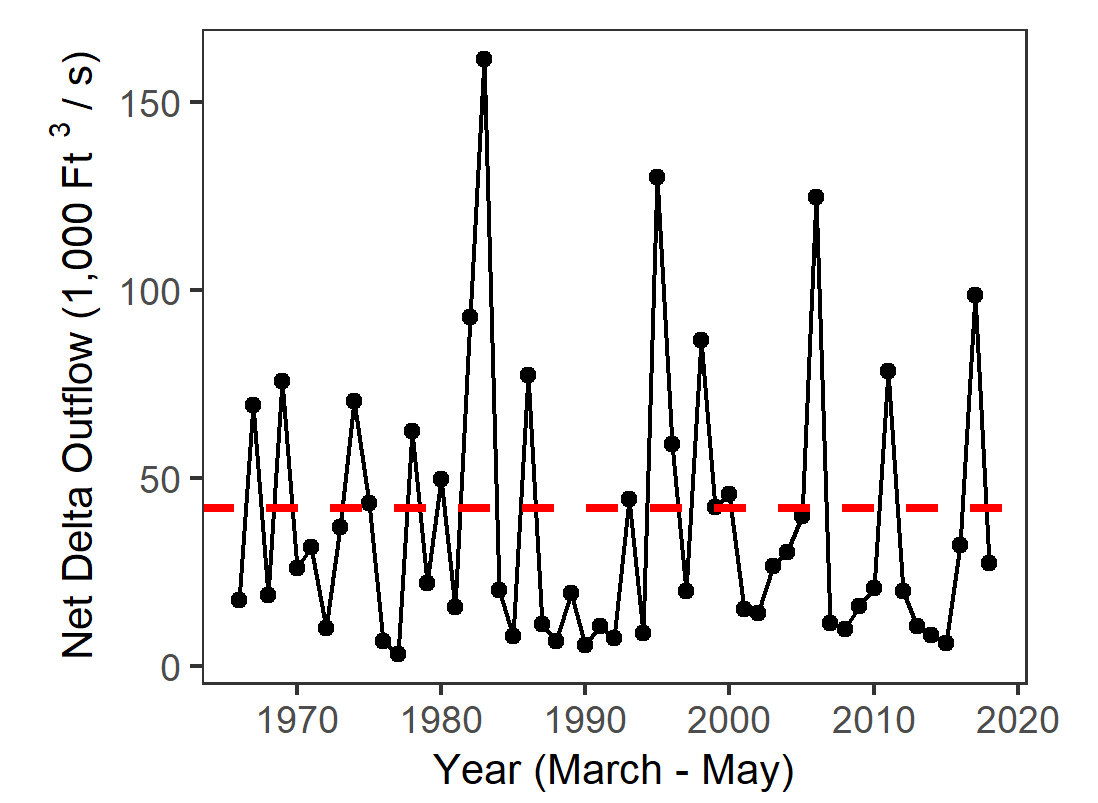
\includegraphics[width=15.25in]{figures/spring_outflow_update}

\begin{itemize}
\tightlist
\item
  Freshwater flow influences water quality, plankton, and fish populations.
\item
  Spring flow is driven primarily by rainfall, snowmelt, and upstream dam releases.
\item
  The spring of 2018 had slightly lower outflow than average.
\end{itemize}

\begin{center}\rule{0.5\linewidth}{0.5pt}\end{center}

\hypertarget{spring-secchi-depth}{%
\section{Spring Secchi Depth}\label{spring-secchi-depth}}

\begin{columns2}

\begin{column}

\hypertarget{background}{%
\subsection{Background}\label{background}}

\begin{itemize}
\tightlist
\item
  Organisms in this ecosystem are adapted to high turbidity conditions, and reductions in turbidity can have many negative ecological effects.
\item
  Higher values for Secchi depth indicate lower turbidity.
\item
  Secchi depth is measured monthly by DWR's \href{https://emp.baydeltalive.com/wiki/12297}{Environmental Monitoring Program} by dropping a black-and-white disk in the water until it disappears.
\end{itemize}

\end{column}

\begin{column}

\begin{figure}

{\centering 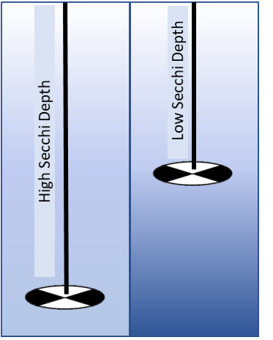
\includegraphics[width=3.79in]{figures/secchidisc} 

}

\caption{image of a secchi disk}\label{fig:unnamed-chunk-6}
\end{figure}

\end{column}

\end{columns2}

\hypertarget{average-secchi-depth-by-region}{%
\subsection{Average Secchi Depth by Region}\label{average-secchi-depth-by-region}}

\begin{columns-nocenter}

\begin{column}

\begin{figure}

\includegraphics[width=15.25in]{figures/mline} \caption{mean is represented by a dotted red line}\label{fig:unnamed-chunk-7}
\end{figure}

\end{column}

\begin{column}

\end{column}

\begin{column}

\end{column}

\end{columns-nocenter}

\begin{panel-grid}

\begin{columns-nocenter}

\begin{column800}

\textbf{San Pablo Bay}

\end{column800}

\begin{column40}

~

\end{column40}

\begin{column800}

\textbf{Suisun}

\end{column800}

\begin{column40}

~

\end{column40}

\begin{column800}

\textbf{Delta}

\end{column800}

\end{columns-nocenter}

\begin{columns-nocenter}

\begin{column800}

\begin{expand}

\begin{figure}
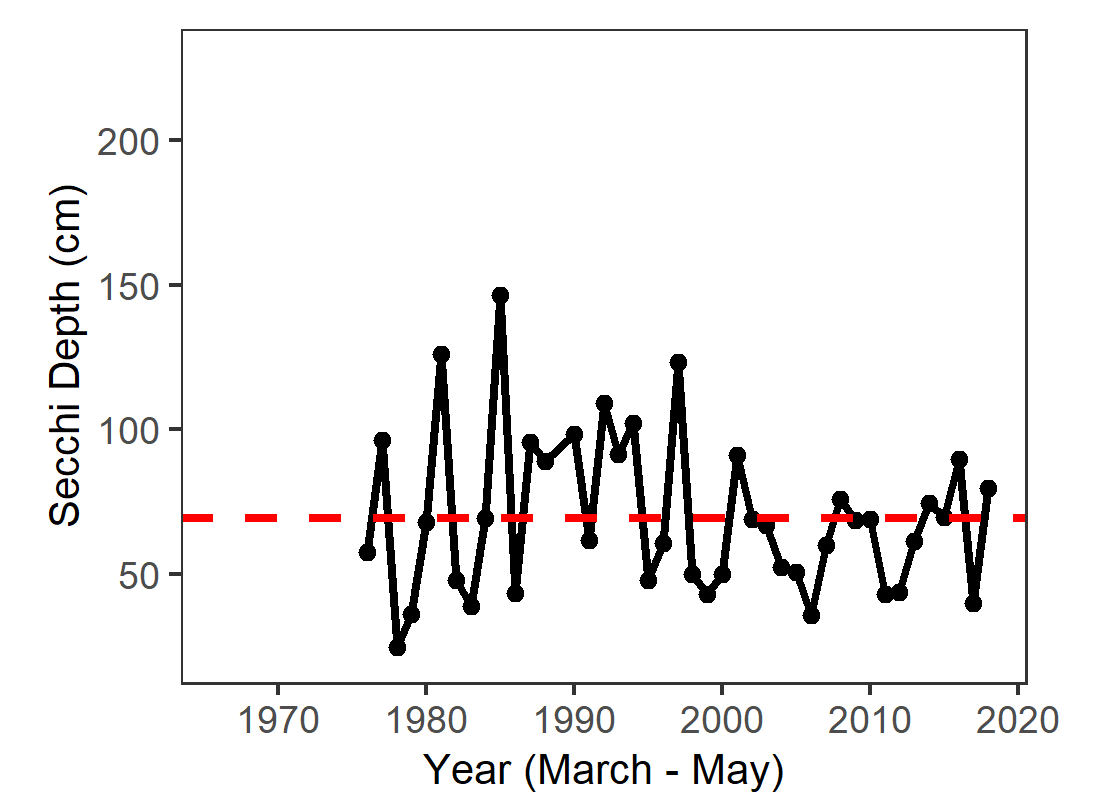
\includegraphics[width=15.25in]{figures/secchi_splspring} \caption{Graph of average spring secchi depth in San Pablo Bay from 1975 to 2018. Values range from 10 to 150.}\label{fig:unnamed-chunk-8}
\end{figure}

\end{expand}

\end{column800}

\begin{column40}

~

\end{column40}

\begin{column800}

\begin{expand}

\begin{figure}
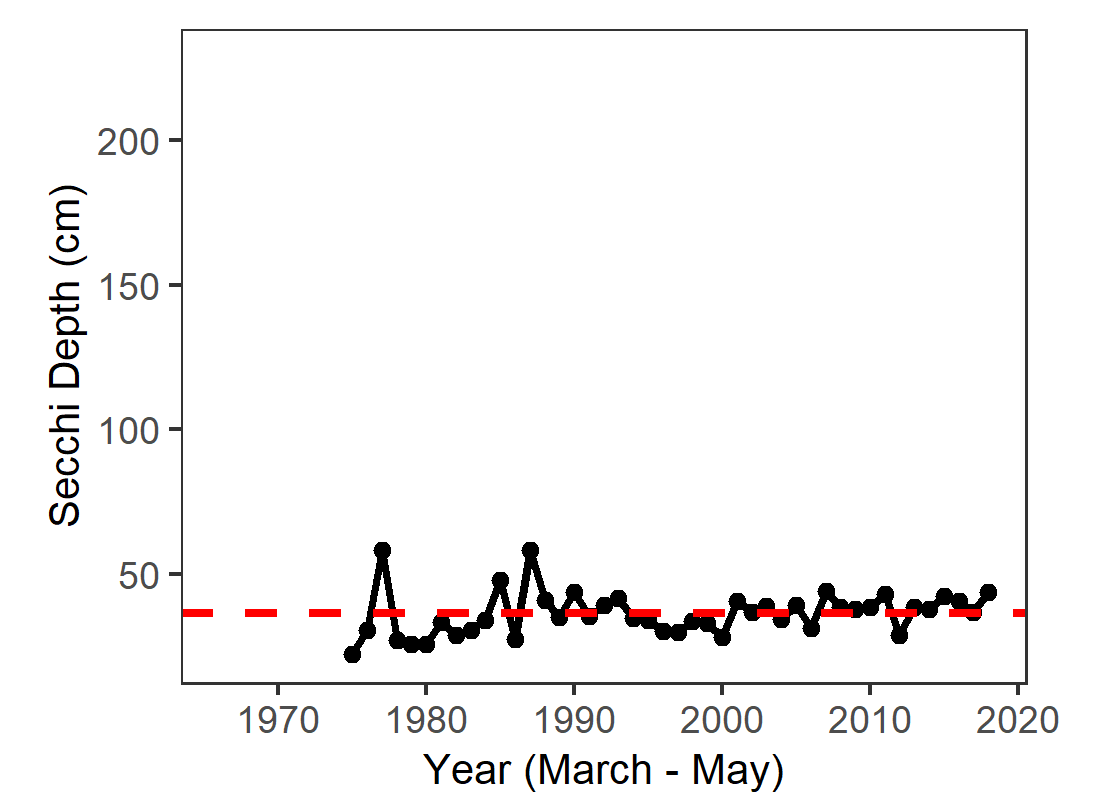
\includegraphics[width=15.25in]{figures/secchi_ssspring} \caption{Graph of average spring secchi depth in Suisun from 1975 to 2018. Values range from 10 to 60.}\label{fig:unnamed-chunk-9}
\end{figure}

\end{expand}

\end{column800}

\begin{column40}

~

\end{column40}

\begin{column800}

\begin{expand}

\begin{figure}
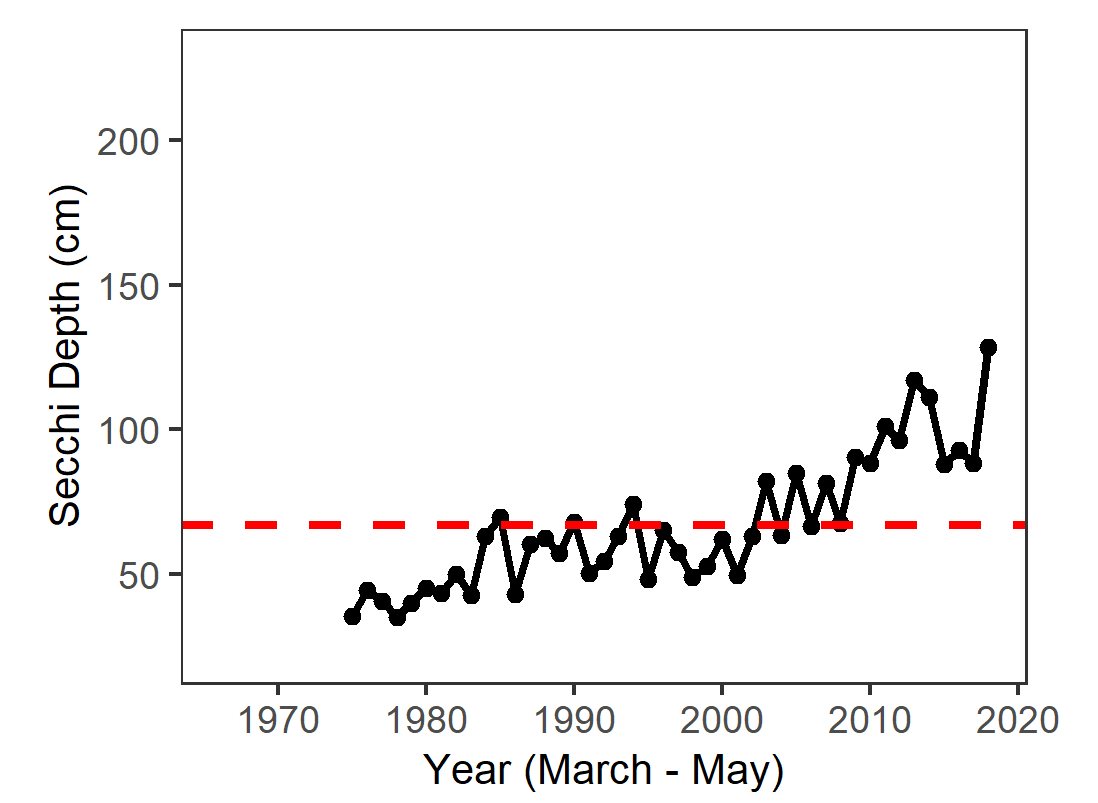
\includegraphics[width=15.25in]{figures/secchi_dtspring} \caption{Graph of average spring secchi depth in the Delta from 1975 to 2018. Values range from 25 to 120 and have been increasing since the year 2000.}\label{fig:unnamed-chunk-10}
\end{figure}

\end{expand}

\end{column800}

\end{columns-nocenter}

\begin{columns-nocenter}

\begin{column800}

In 2018, San Pablo bay was close to the long-term average.

\end{column800}

\begin{column40}

~

\end{column40}

\begin{column800}

In 2018, Suisun Bay was also close to the long-term average

\end{column800}

\begin{column40}

~

\end{column40}

\begin{column800}

In 2018, the Delta was much clearer than average, the clearest Spring on record.

\end{column800}

\end{columns-nocenter}

\end{panel-grid}

\begin{disclaimer}
\href{https://link.springer.com/article/10.1007/s12237-011-9382-x}{Schoellhamer,
D. H. 2011. Sudden clearing of estuarine waters upon crossing the
threshold from transport to supply regulation of sediment transport as
an erodible sediment pool is depleted: San Francisco Bay, 1999.
Estuaries and Coasts 34(5):885-899.}
\end{disclaimer}

\begin{center}\rule{0.5\linewidth}{0.5pt}\end{center}

\hypertarget{spring-water-temperature}{%
\section{Spring Water Temperature}\label{spring-water-temperature}}

\begin{columns-nocenter}

\begin{column}

\hypertarget{background-1}{%
\subsection{Background}\label{background-1}}

\begin{itemize}
\tightlist
\item
  Water temperature is monitored monthly by DWR's \href{https://emp.baydeltalive.com/wiki/12297}{Environmental Monitoring Program}.
\item
  Fish growth and reproduction is highest in certain temperature ranges.
\item
  Increasing Spring temperatures may lower Delta Smelt reproduction.
\item
  Temperatures tend to be similar between regions in the spring.
\end{itemize}

\end{column}

\begin{column}

\begin{figure}

{\centering 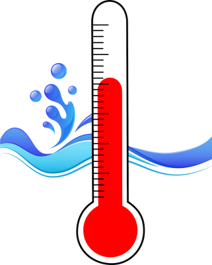
\includegraphics[width=2.94in]{figures/thermometer} 

}

\caption{picture of a thermometer in water}\label{fig:unnamed-chunk-12}
\end{figure}

\end{column}

\end{columns-nocenter}

\hypertarget{average-temperature-by-region}{%
\subsection{Average Temperature by Region}\label{average-temperature-by-region}}

\begin{columns-nocenter}

\begin{column}

\begin{figure}

\includegraphics[width=15.25in]{figures/mline} \caption{mean is represented by a dotted red line}\label{fig:unnamed-chunk-13}
\end{figure}

\end{column}

\begin{column}

\end{column}

\begin{column}

\end{column}

\end{columns-nocenter}

\begin{panel-grid}

\begin{columns-nocenter}

\begin{column800}

\textbf{San Pablo Bay}

\end{column800}

\begin{column40}

~

\end{column40}

\begin{column800}

\textbf{Suisun}

\end{column800}

\begin{column40}

~

\end{column40}

\begin{column800}

\textbf{Delta}

\end{column800}

\end{columns-nocenter}

\begin{columns-nocenter}

\begin{column800}

\begin{expand}

\begin{figure}
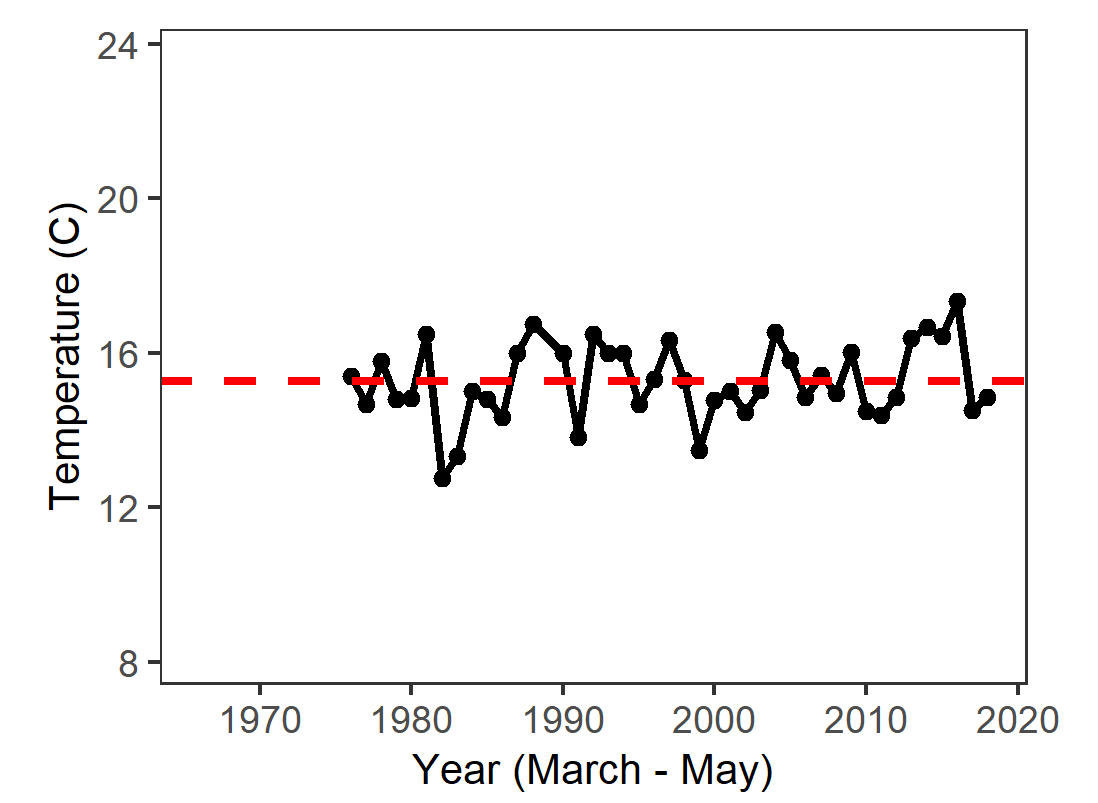
\includegraphics[width=15.25in]{figures/temp_splspring} \caption{Graph of average spring water temperature in San Pablo Bay from 1975 to 2018. Values range from 13 to 18.}\label{fig:unnamed-chunk-14}
\end{figure}

\end{expand}

\end{column800}

\begin{column40}

~

\end{column40}

\begin{column800}

\begin{expand}

\begin{figure}
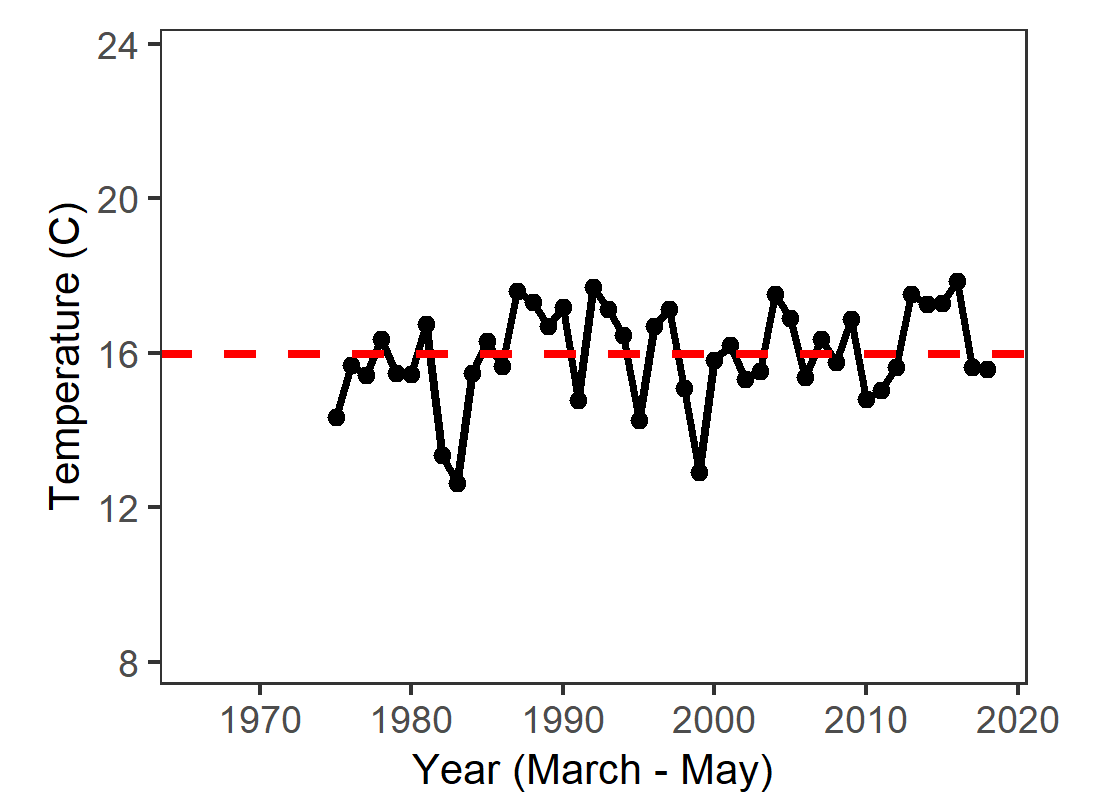
\includegraphics[width=15.25in]{figures/temp_ssspring} \caption{Graph of average spring water temperature in Suisun from 1975 to 2018. Values range from 13 to 18.}\label{fig:unnamed-chunk-15}
\end{figure}

\end{expand}

\end{column800}

\begin{column40}

~

\end{column40}

\begin{column800}

\begin{expand}

\begin{figure}
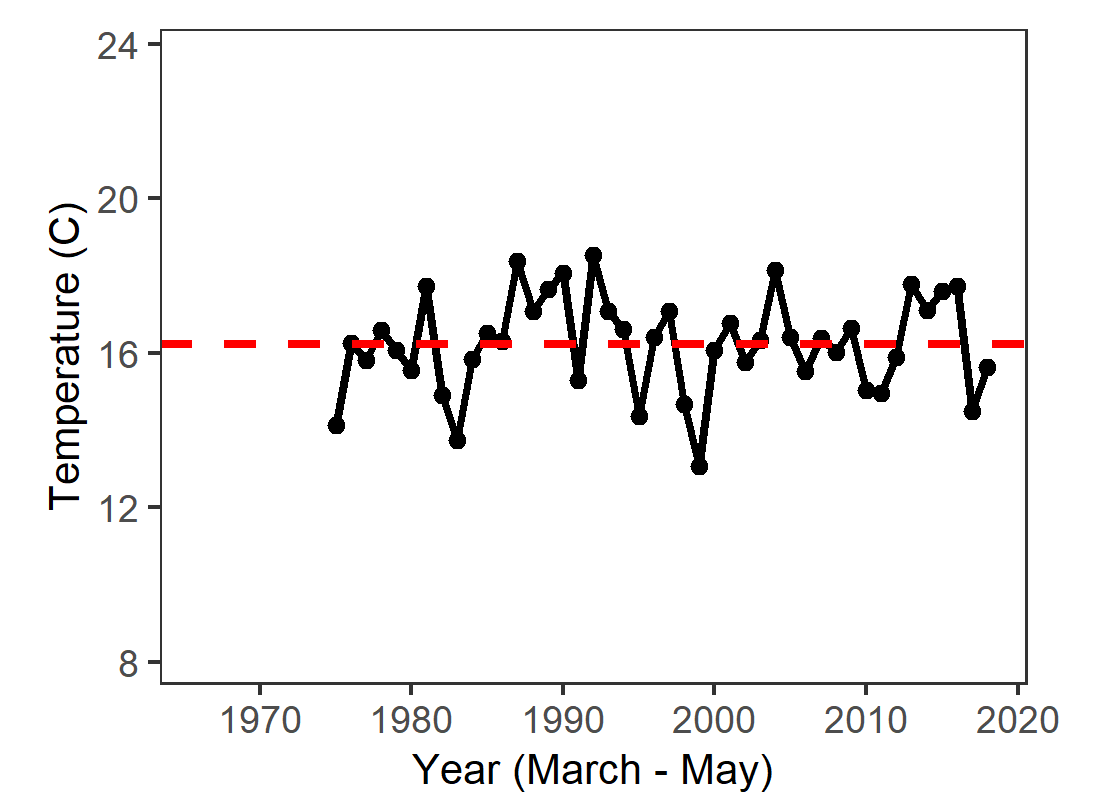
\includegraphics[width=15.25in]{figures/temp_dtspring} \caption{Graph of average spring water temperature in the Delta from 1975 to 2018. Values range from 13 to 18.}\label{fig:unnamed-chunk-16}
\end{figure}

\end{expand}

\end{column800}

\end{columns-nocenter}

\begin{columns-nocenter}

\begin{column800}

In 2018, San Pablo Bay temperatures were similar to the long-term average.

\end{column800}

\begin{column40}

~

\end{column40}

\begin{column800}

In 2018, Suisun Bay was similar to the long-term average.

\end{column800}

\begin{column40}

~

\end{column40}

\begin{column800}

In 2018, the Delta was slightly cooler than average.

\end{column800}

\end{columns-nocenter}

\end{panel-grid}

\begin{disclaimer}
For more information see: Jeffries, et al.. 2016. Effects of high
temperatures on threatened estuarine fishes during periods of extreme
drought. The Journal of Experimental Biology 219(11):1705-1716.
\end{disclaimer}

\begin{center}\rule{0.5\linewidth}{0.5pt}\end{center}

\hypertarget{spring-chlorophyll}{%
\section{Spring Chlorophyll}\label{spring-chlorophyll}}

\begin{columns-nocenter}

\begin{column}

\hypertarget{background-2}{%
\subsection{Background}\label{background-2}}

\begin{itemize}
\tightlist
\item
  Chlorophyll is an indicator of phytoplankton production, which is low during the Spring.
\item
  Phytoplankton are the base of the pelagic food web. It is sampled monthly by DWR's \href{https://emp.baydeltalive.com/wiki/12297}{Environmental Monitoring Program}.
\item
  The invasion of the clam \emph{Potamocorbula amurensis} caused a decline in phytoplankton and zooplankton after 1986 -- especially in Suisun Bay.
\end{itemize}

\end{column}

\begin{column}

\begin{figure}

{\centering 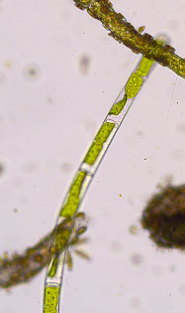
\includegraphics[width=2.57in]{figures/phyto} 

}

\caption{picture of phytoplankton}\label{fig:unnamed-chunk-18}
\end{figure}

\end{column}

\end{columns-nocenter}

\hypertarget{average-chlorophyll-by-region}{%
\subsection{Average Chlorophyll by Region}\label{average-chlorophyll-by-region}}

\begin{columns-nocenter}

\begin{column}

\begin{figure}

\includegraphics[width=15.25in]{figures/mline} \caption{mean is represented by a dotted red line}\label{fig:unnamed-chunk-19}
\end{figure}

\end{column}

\begin{column}

\end{column}

\begin{column}

\end{column}

\end{columns-nocenter}

\begin{panel-grid}

\begin{columns-nocenter}

\begin{column800}

\textbf{San Pablo Bay}

\end{column800}

\begin{column40}

~

\end{column40}

\begin{column800}

\textbf{Suisun}

\end{column800}

\begin{column40}

~

\end{column40}

\begin{column800}

\textbf{Delta}

\end{column800}

\end{columns-nocenter}

\begin{columns-nocenter}

\begin{column800}

\begin{expand}

\begin{figure}
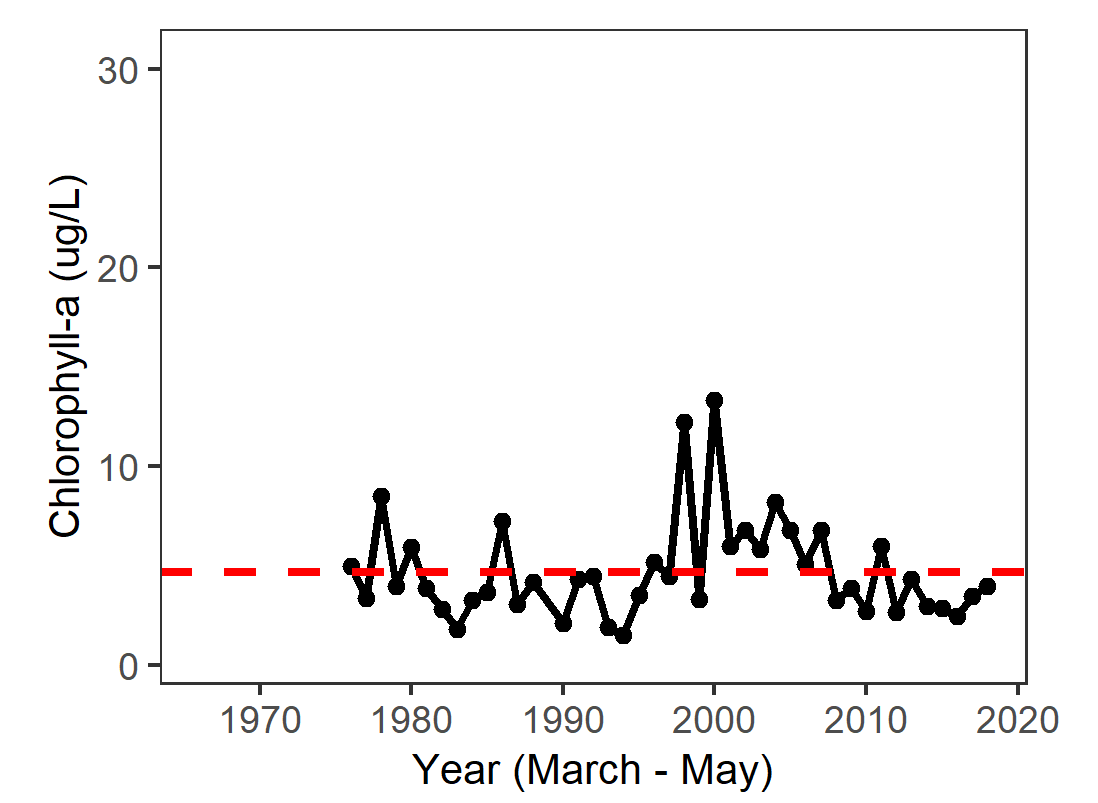
\includegraphics[width=15.25in]{figures/chla_splspring} \caption{Graph of average spring chlorophyll in San Pablo Bay from 1975 to 2018. Values range from 4 to 15.}\label{fig:unnamed-chunk-20}
\end{figure}

\end{expand}

\end{column800}

\begin{column40}

~

\end{column40}

\begin{column800}

\begin{expand}

\begin{figure}
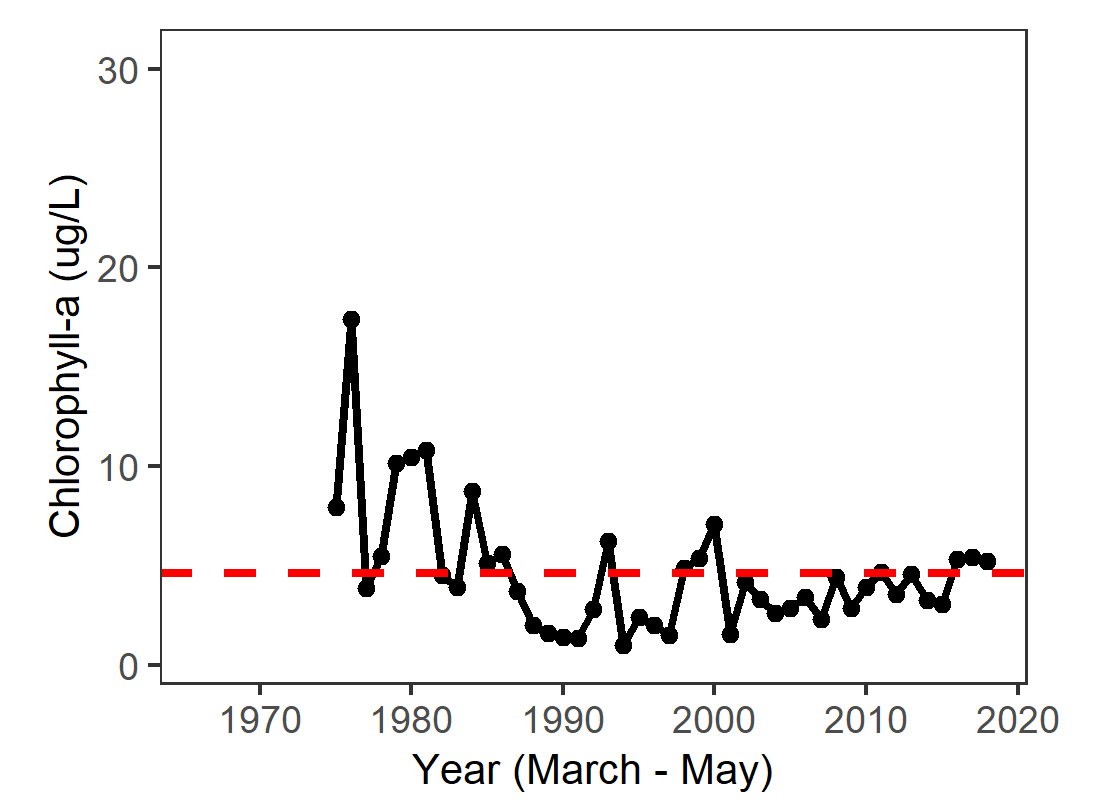
\includegraphics[width=15.25in]{figures/chla_ssspring} \caption{Graph of average spring chlorophyll in Suisun from 1975 to 2018. Values range from 2 to 19.}\label{fig:unnamed-chunk-21}
\end{figure}

\end{expand}

\end{column800}

\begin{column40}

~

\end{column40}

\begin{column800}

\begin{expand}

\begin{figure}
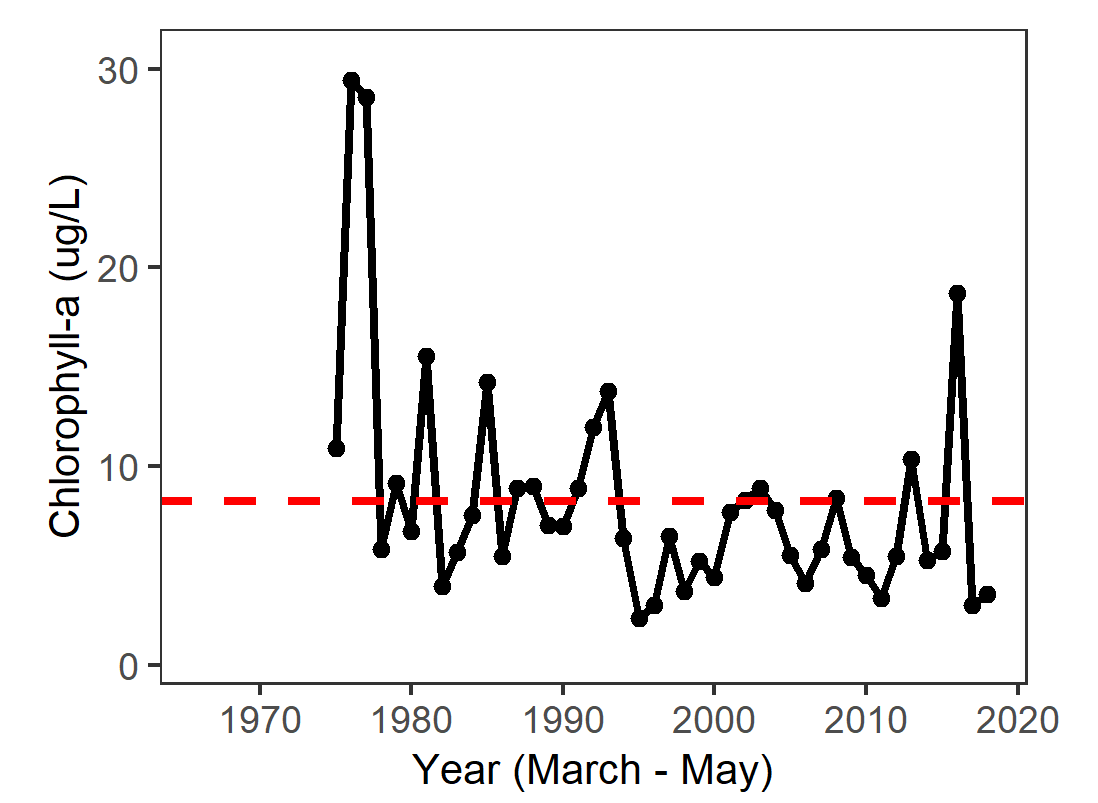
\includegraphics[width=15.25in]{figures/chla_dtspring} \caption{Graph of average spring chlorophyll in the Delta from 1975 to 2018. Values range from 3.5 to 29.}\label{fig:unnamed-chunk-22}
\end{figure}

\end{expand}

\end{column800}

\end{columns-nocenter}

\begin{columns-nocenter}

\begin{column800}

In 2018, San Pablo Bay chlorophyll was similar to the long-term average.

\end{column800}

\begin{column40}

~

\end{column40}

\begin{column800}

In 2018, Suisun Bay chlorophyll was also about average.

\end{column800}

\begin{column40}

~

\end{column40}

\begin{column800}

In 2018, the Delta had lower chlorophyll than average.

\end{column800}

\end{columns-nocenter}

\end{panel-grid}

\begin{disclaimer}
For more information see: Cahoon, T. and T. Brown. 2018. Phytoplankton,
Chlorophyll-a and Pheophytin-a Status and Trends 2017. IEP Newsletter
32(1):14-20.
\end{disclaimer}

\begin{center}\rule{0.5\linewidth}{0.5pt}\end{center}

\hypertarget{spring-zooplankton}{%
\section{Spring Zooplankton}\label{spring-zooplankton}}

\begin{columns-nocenter}

\begin{column}

\hypertarget{background-3}{%
\subsection{Background}\label{background-3}}

\begin{itemize}
\tightlist
\item
  Zooplankton is sampled monthly by the CDFW/DWR \href{https://emp.baydeltalive.com/wiki/12297}{Environmental Monitoring Program} but sampling in San Pablo Bay did not begin until 1998.
\item
  Zooplankton are an important food source for pelagic fish.
\item
  Calanoid copepods and mysids are particularly good fish food. Cyclopoid copepods are not as good for fish food.
\item
  Biomass in Spring tends to be higher than Winter, but lower than Summer.
\end{itemize}

\end{column}

\begin{column}

Copepod

\begin{figure}

{\centering 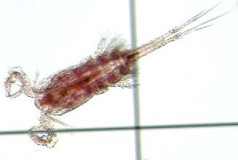
\includegraphics[width=3.31in]{figures/copepod} 

}

\caption{picture of a copepod}\label{fig:unnamed-chunk-24}
\end{figure}

Mysid

\begin{figure}

{\centering 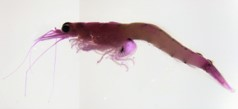
\includegraphics[width=3.31in]{figures/mysid} 

}

\caption{picture of a copepod}\label{fig:unnamed-chunk-25}
\end{figure}

\end{column}

\end{columns-nocenter}

\hypertarget{average-zooplankton-biomass-by-region}{%
\subsection{Average Zooplankton Biomass by Region}\label{average-zooplankton-biomass-by-region}}

\begin{columns-nocenter}

\begin{column}

\begin{figure}

\includegraphics[width=15.25in]{figures/mline} \caption{mean is represented by a dotted red line}\label{fig:unnamed-chunk-26}
\end{figure}

\end{column}

\begin{column}

\end{column}

\begin{column}

\end{column}

\end{columns-nocenter}

\begin{panel-grid}

\begin{columns-nocenter}

\begin{column800}

\textbf{San Pablo Bay}

\end{column800}

\begin{column40}

~

\end{column40}

\begin{column800}

\textbf{Suisun}

\end{column800}

\begin{column40}

~

\end{column40}

\begin{column800}

\textbf{Delta}

\end{column800}

\end{columns-nocenter}

\begin{columns-nocenter}

\begin{column800}

\begin{expand}

\begin{figure}
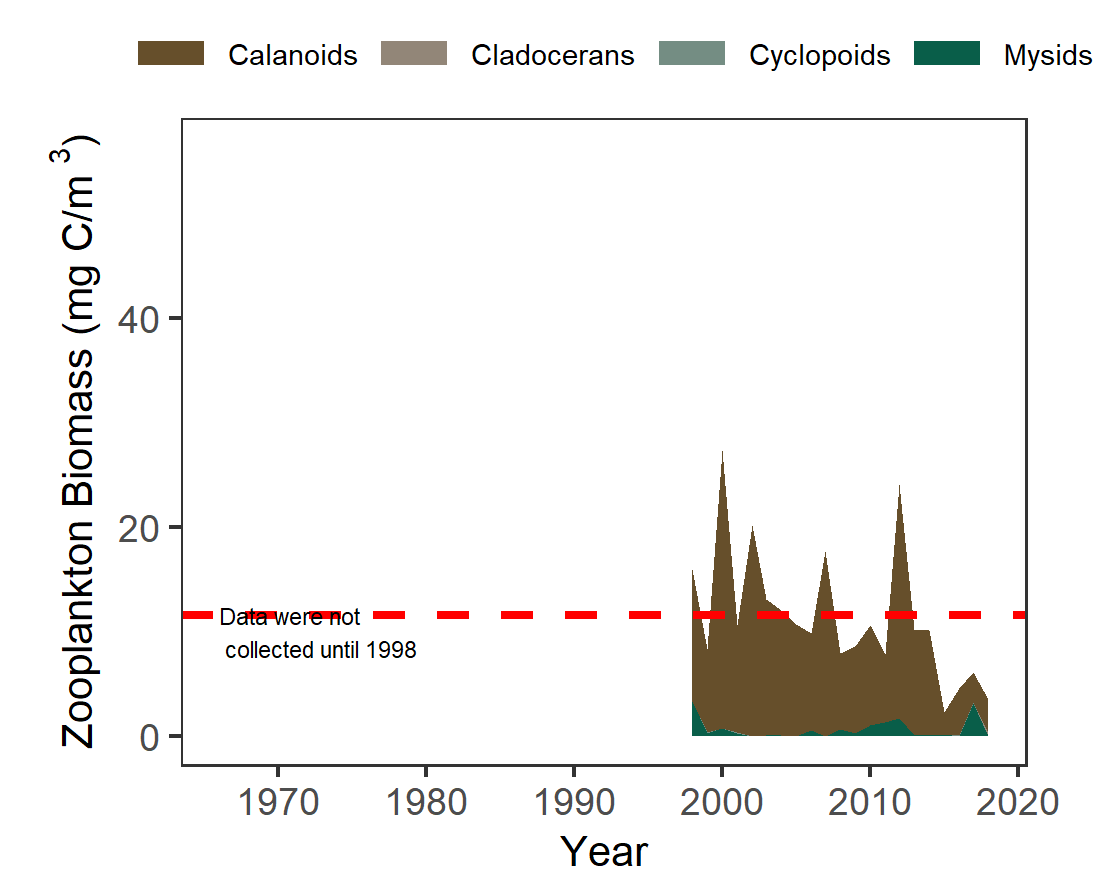
\includegraphics[width=15.25in]{figures/zoops_splspring} \caption{Graph of average spring zooplankton biomass in San Pablo Bay from 1975 to 2018. Values range from 5 to 25.}\label{fig:unnamed-chunk-27}
\end{figure}

\end{expand}

\end{column800}

\begin{column40}

~

\end{column40}

\begin{column800}

\begin{expand}

\begin{figure}
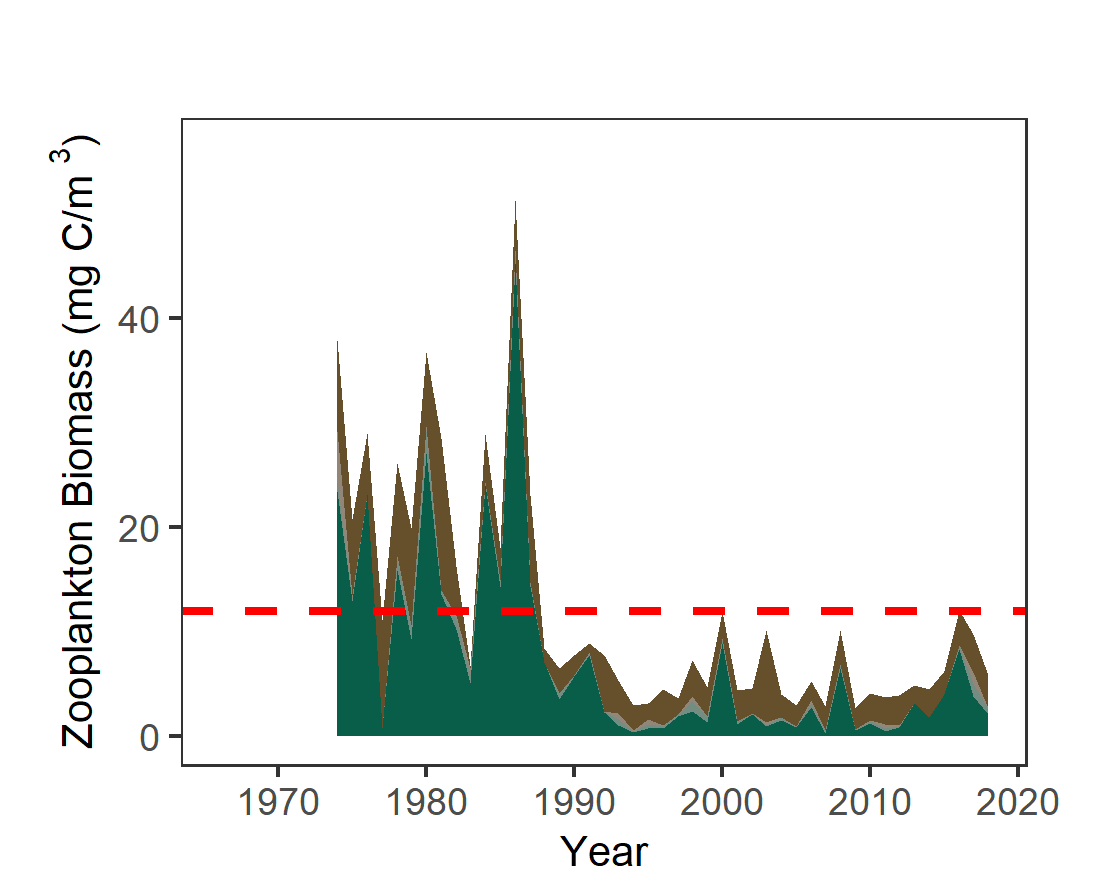
\includegraphics[width=15.25in]{figures/zoops_ssspring} \caption{Graph of average spring chlorophyll in Suisun from 1975 to 2018. Values range from 5 to 45 with much higher biomass before 1986.}\label{fig:unnamed-chunk-28}
\end{figure}

\end{expand}

\end{column800}

\begin{column40}

~

\end{column40}

\begin{column800}

\begin{expand}

\begin{figure}
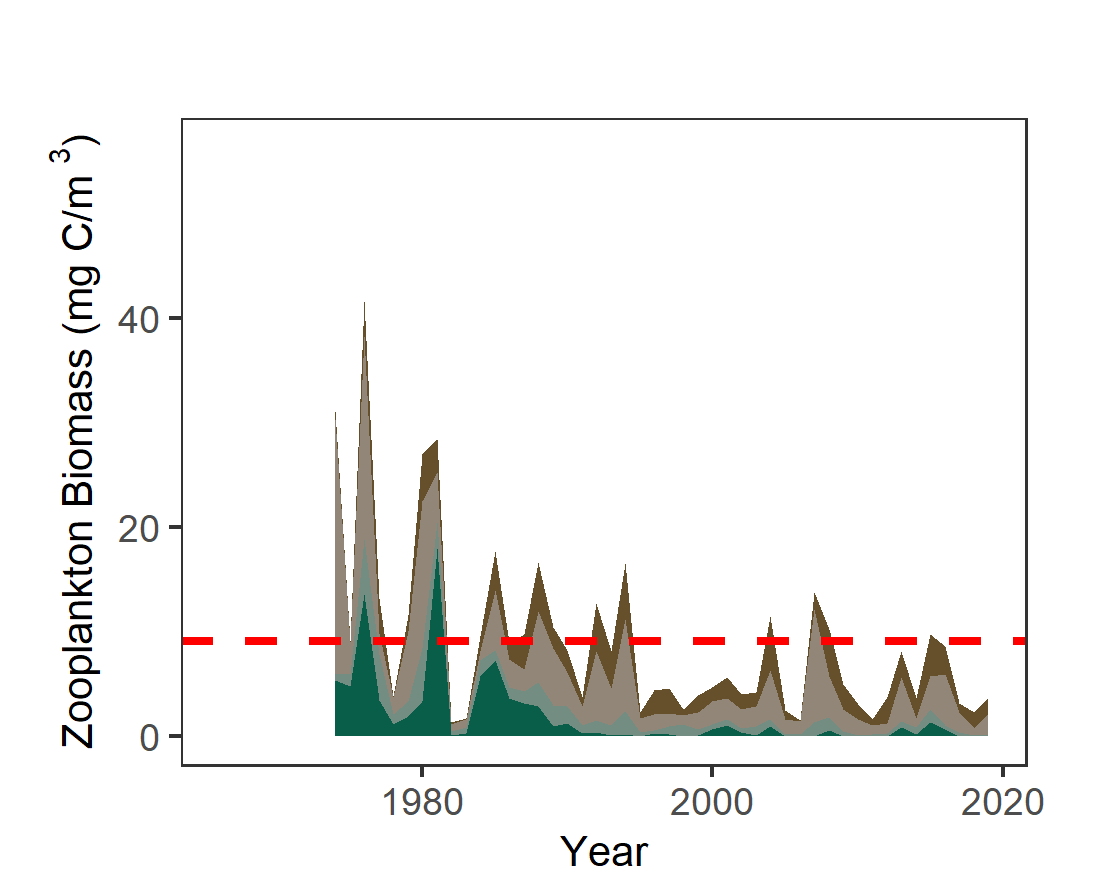
\includegraphics[width=15.25in]{figures/zoops_dtspring} \caption{Graph of average spring zooplankton biomass in the Delta from 1975 to 2018. Values range from 3.5 to 39.}\label{fig:unnamed-chunk-29}
\end{figure}

\end{expand}

\end{column800}

\end{columns-nocenter}

\begin{columns-nocenter}

\begin{column800}

In 2018, San Pablo Bay had much lower than average biomass, mostly calanoid copepods.

\end{column800}

\begin{column40}

~

\end{column40}

\begin{column800}

In 2018, Suisun Bay also had much lower than average total biomass.

\end{column800}

\begin{column40}

~

\end{column40}

\begin{column800}

In 2018, the Delta also had much lower than average total biomass.

\end{column800}

\end{columns-nocenter}

\end{panel-grid}

\begin{disclaimer}
For more information see: Hennessy, A. 2018. Zooplankton Monitoring
2017. IEP Newsletter 32(1):21-32. Available on request:
\href{mailto:iepnewsletter@water.ca.gov}{\nolinkurl{iepnewsletter@water.ca.gov}}
\end{disclaimer}

\begin{center}\rule{0.5\linewidth}{0.5pt}\end{center}

\hypertarget{spring-fish}{%
\section{Spring Fish}\label{spring-fish}}

\hypertarget{background-4}{%
\subsection{Background}\label{background-4}}

\begin{itemize}
\tightlist
\item
  Splittail are a native minnow that spawn on floodplains, so have high reproduction during high flow years when floodplains are inundated with water. Juvenile splittail are sampled by DWR's \href{https://portal.edirepository.org/nis/mapbrowse?packageid=edi.233.2}{Yolo Bypass Monitoring Program}'s rotory screw trap.
\item
  Spring-run Adult salmon return from the ocean during the spring. Populations are calculated by CDFW's \href{http://www.cbr.washington.edu/sacramento/data/query_adult_grandtab.html}{Fisheries Branch} based on redd counts, carcass surveys, fish entering hatcheries, and live fish counts.
\item
  Juvenile Winter-Run Chinook Salmon out-migrate to the ocean in spring, and are sampled by the USFWS's \href{https://www.fws.gov/lodi/juvenile_fish_monitoring_program/jfmp_index.htm}{Chipps Island Trawl}, located at the confluence of the Sacramento and San Joaquin Rivers.
\end{itemize}

\hypertarget{average-fish-catch-trends-by-species}{%
\subsection{Average Fish Catch Trends by Species}\label{average-fish-catch-trends-by-species}}

\begin{columns-nocenter}

\begin{column}

\begin{figure}

\includegraphics[width=15.25in]{figures/mline} \caption{mean is represented by a dotted red line}\label{fig:unnamed-chunk-31}
\end{figure}

\end{column}

\begin{column}

\end{column}

\begin{column}

\end{column}

\end{columns-nocenter}

\begin{panel-grid}

\begin{columns-nocenter}

\begin{column800}

\textbf{\href{http://calfish.ucdavis.edu/species/?uid=136\&ds=698}{Juvenile Sacramento Splittail}}

\end{column800}

\begin{column40}

~

\end{column40}

\begin{column800}

\textbf{\href{http://calfish.ucdavis.edu/species/?uid=28\&ds=698}{Adult Spring-Run Chinook}}

\end{column800}

\begin{column40}

~

\end{column40}

\begin{column800}

\textbf{\href{http://calfish.ucdavis.edu/species/?uid=30\&ds=698}{Juvenile Winter-Run Chinook}}

\end{column800}

\end{columns-nocenter}

\begin{columns-nocenter}

\begin{column800}

\begin{figure}

{\centering 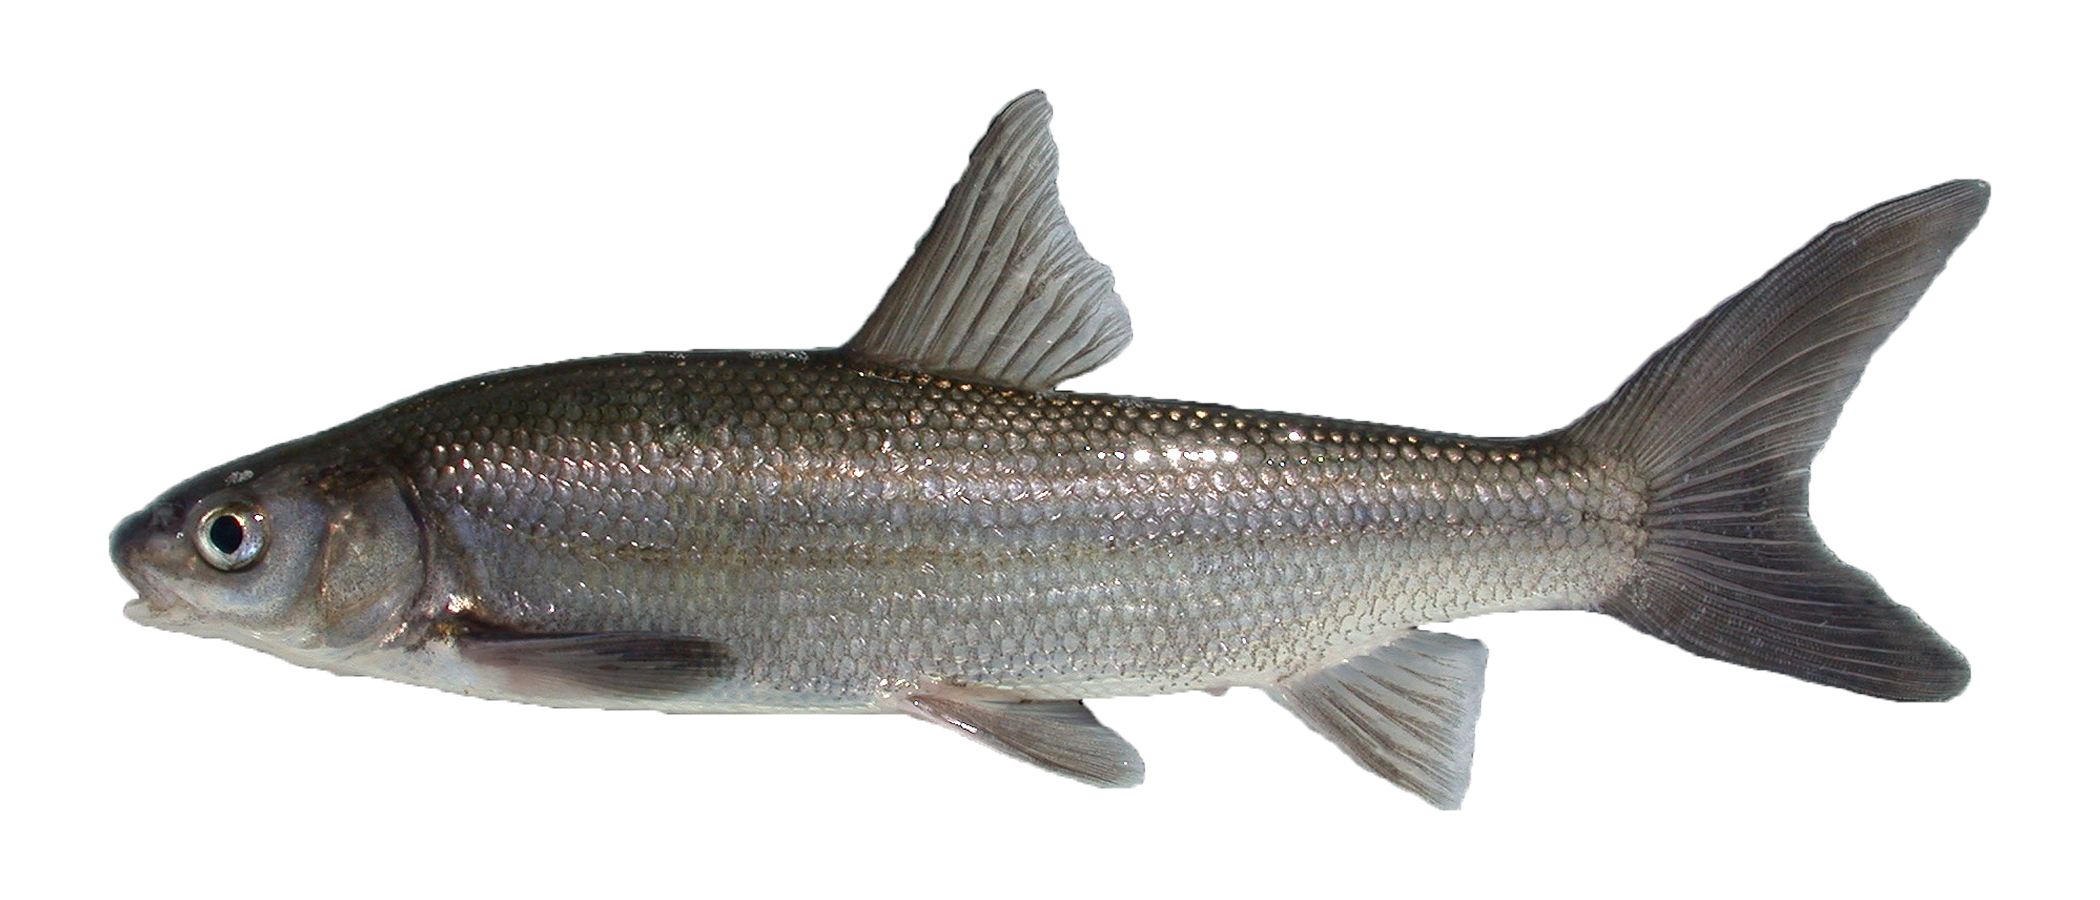
\includegraphics[width=29.17in]{figures/splittail_adult} 

}

\caption{picture of a sacramento splittail}\label{fig:unnamed-chunk-32}
\end{figure}

\end{column800}

\begin{column40}

~

\end{column40}

\begin{column800}

\begin{figure}

{\centering 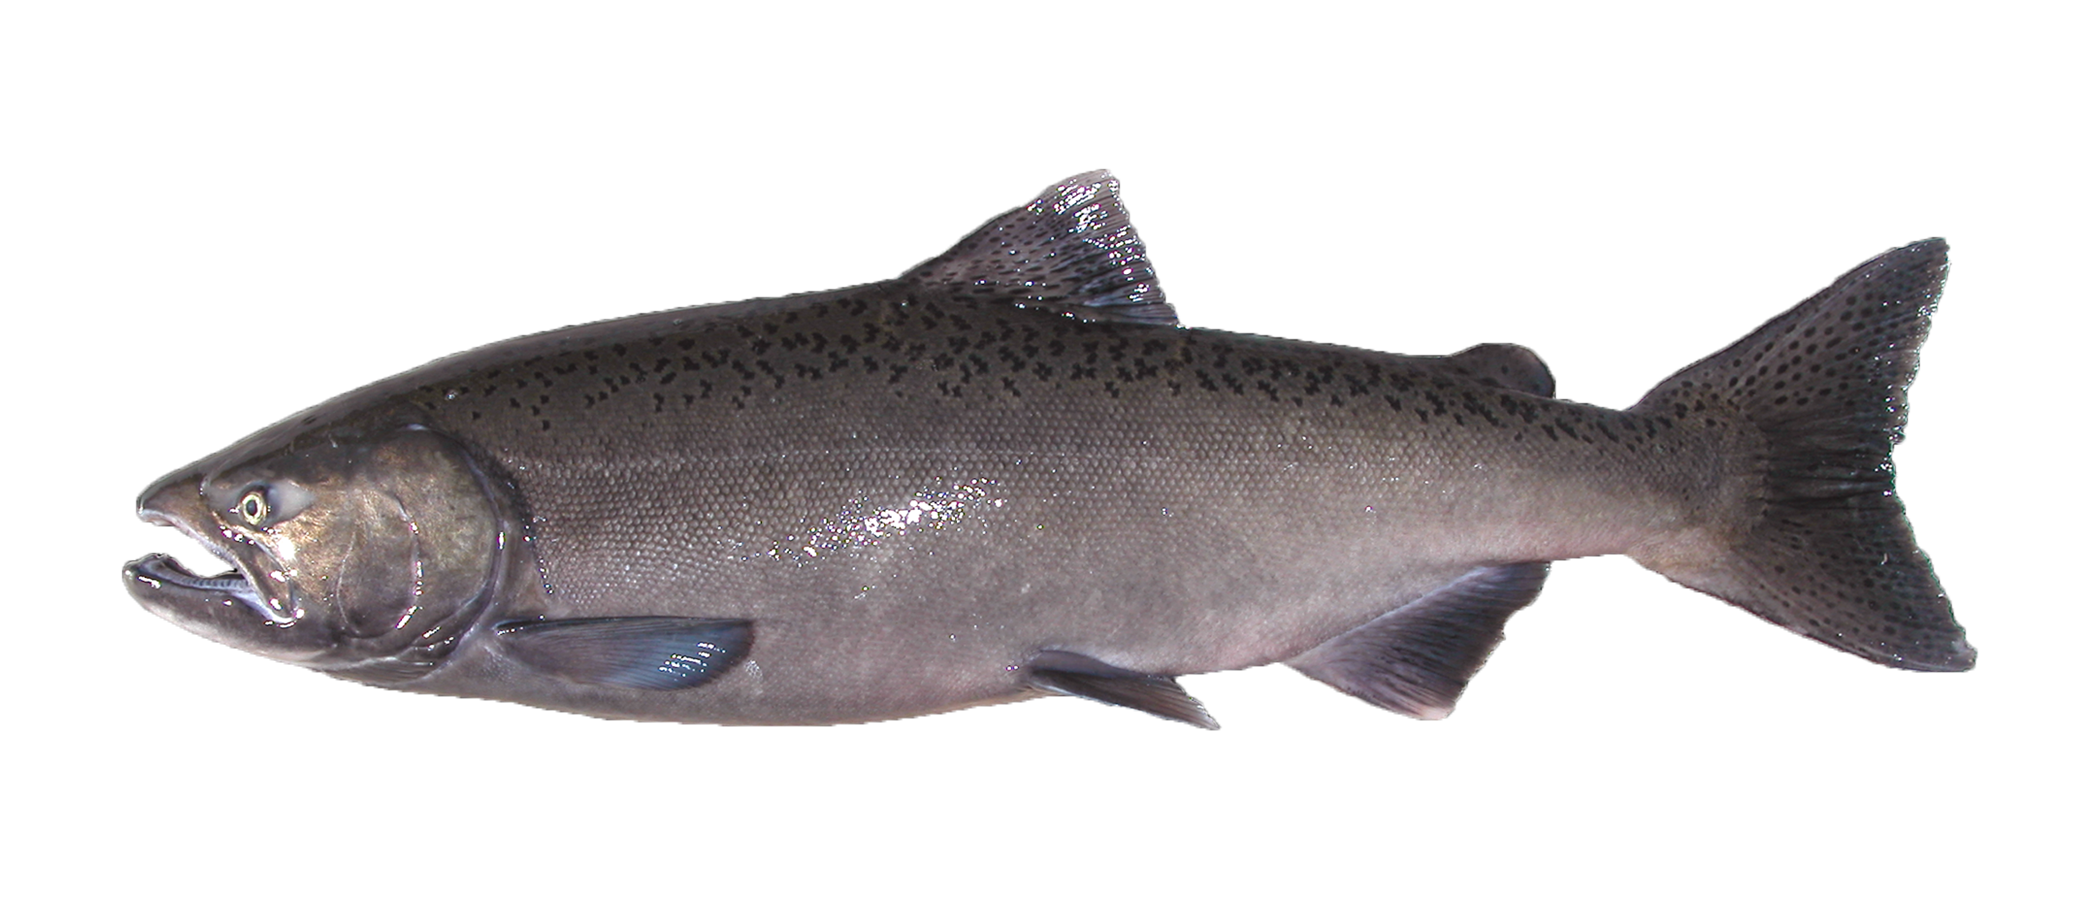
\includegraphics[width=29.17in]{figures/chinook_salmon} 

}

\caption{picture of an adults chinook salmon}\label{fig:unnamed-chunk-33}
\end{figure}

\end{column800}

\begin{column40}

~

\end{column40}

\begin{column800}

\begin{figure}

{\centering 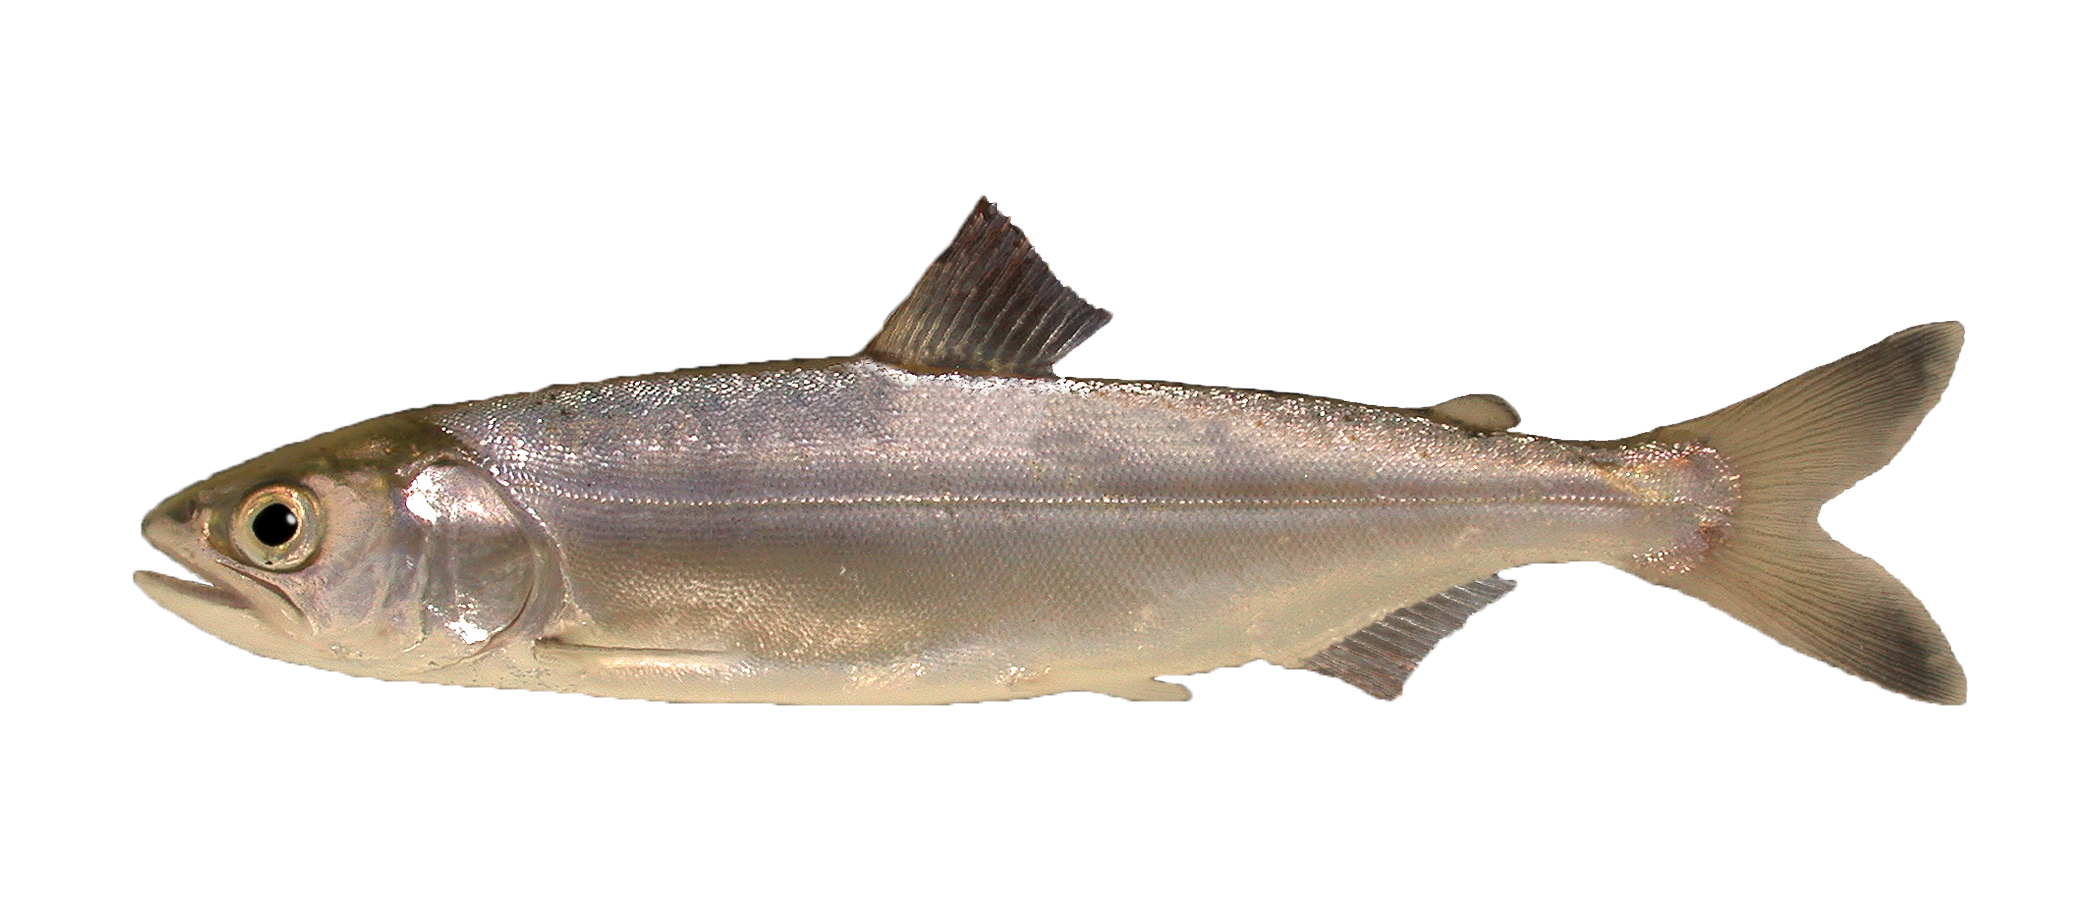
\includegraphics[width=29.17in]{figures/chinook_salmon_smolt} 

}

\caption{picture of a juvenile salmon}\label{fig:unnamed-chunk-34}
\end{figure}

\end{column800}

\end{columns-nocenter}

\begin{columns-nocenter}

\begin{column800}

\begin{expand}

\begin{figure}
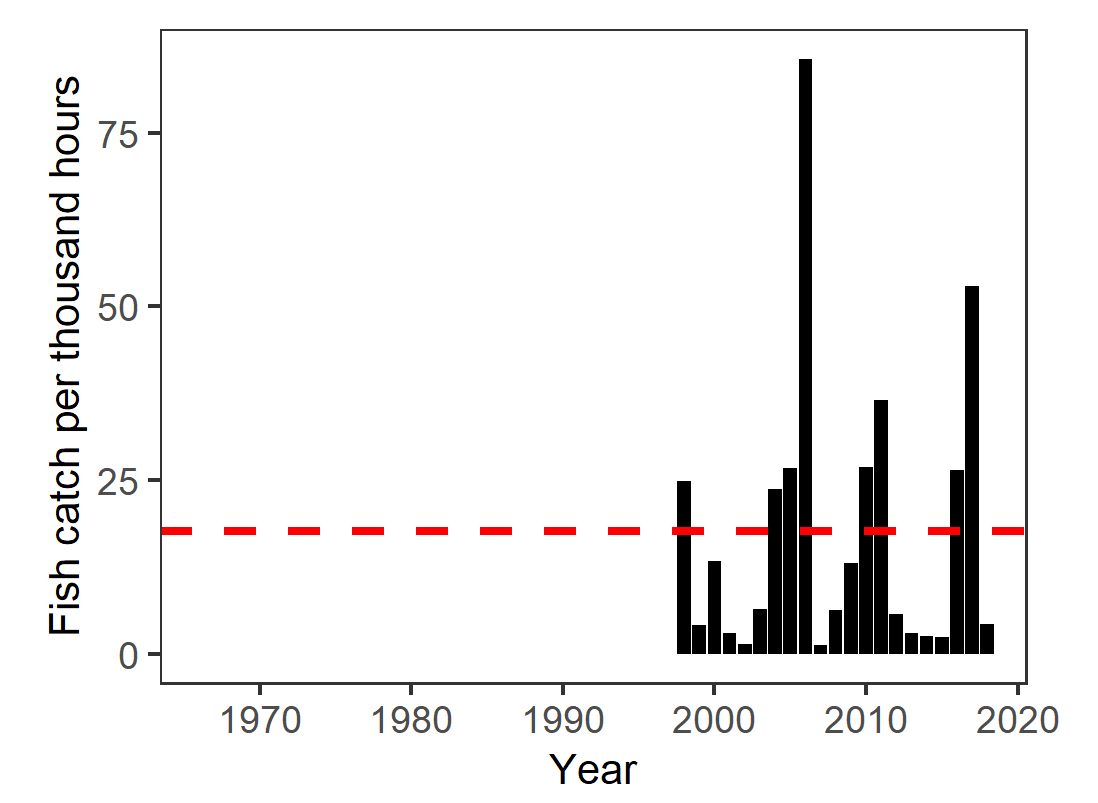
\includegraphics[width=15.25in]{figures/yolo_splittail} \caption{Graph of average Sacramento Splittail catch per unit effort from 1998 to 2018. Values range from 4 to 80.}\label{fig:unnamed-chunk-35}
\end{figure}

\end{expand}

\end{column800}

\begin{column40}

~

\end{column40}

\begin{column800}

\begin{expand}

\begin{figure}
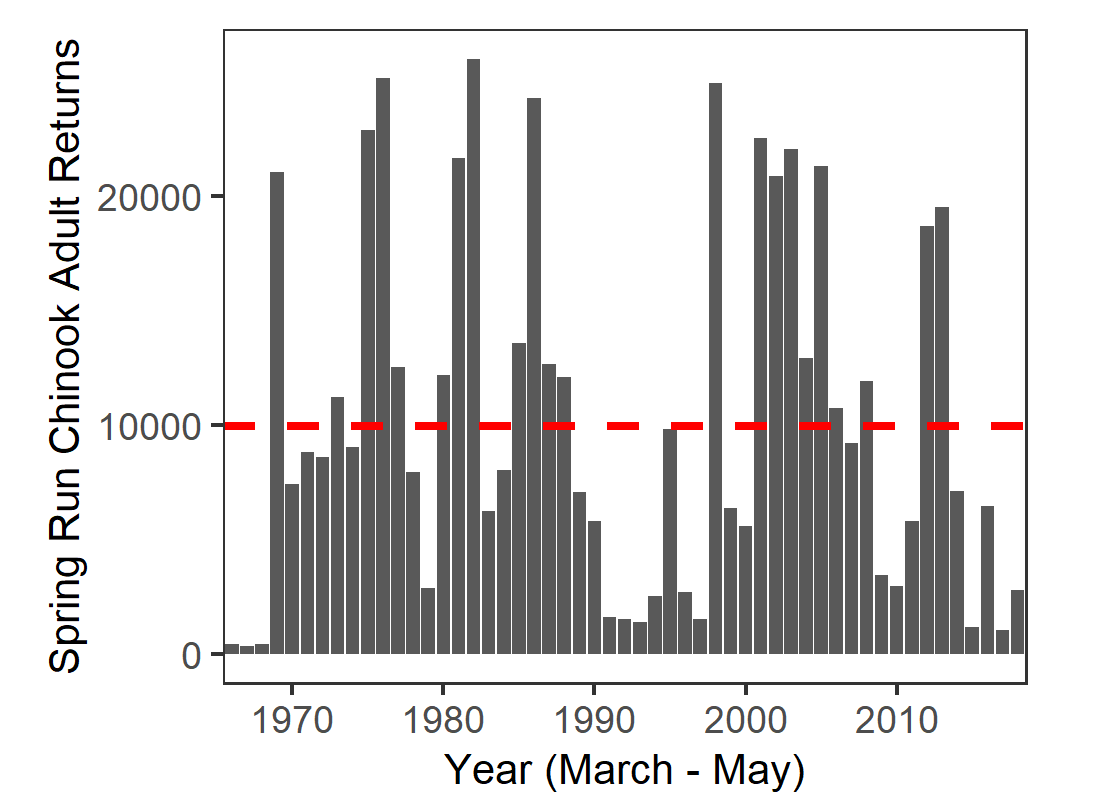
\includegraphics[width=15.25in]{figures/SpringRun_1966} \caption{Graph of average adult chinook returns from 1966 to 2018. Values range from 1000 to 250000.}\label{fig:unnamed-chunk-36}
\end{figure}

\end{expand}

\end{column800}

\begin{column40}

~

\end{column40}

\begin{column800}

\begin{expand}

\begin{figure}
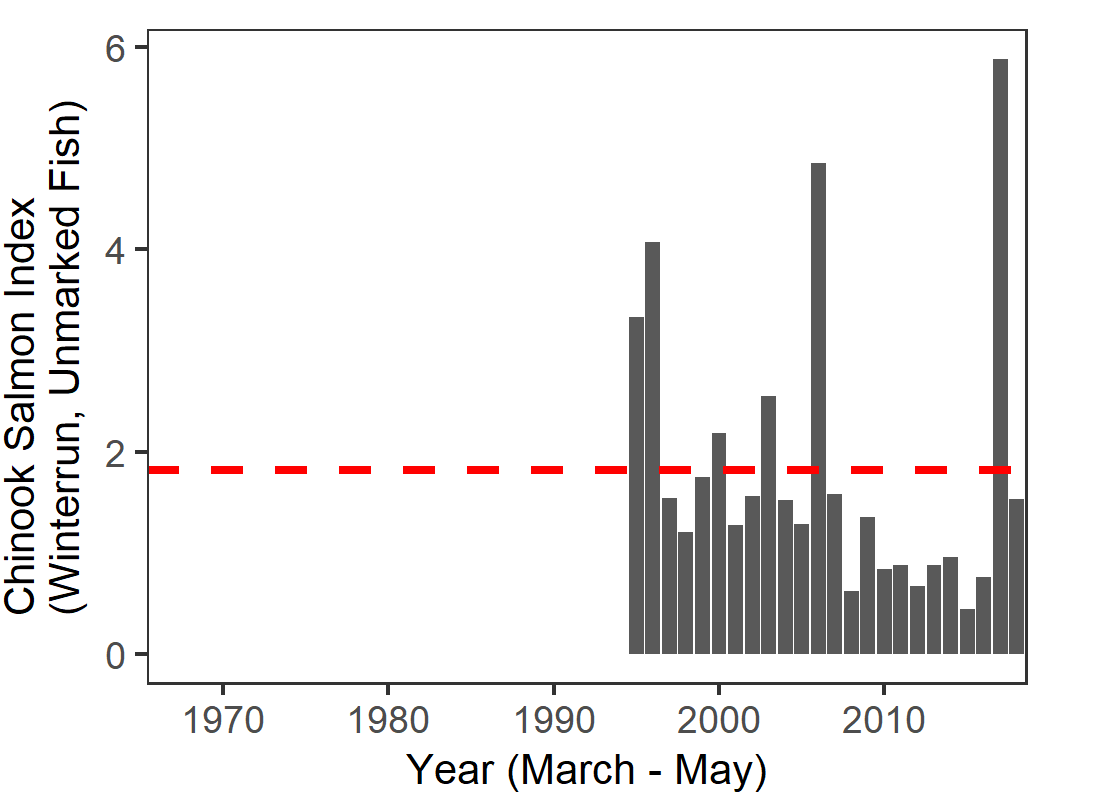
\includegraphics[width=15.25in]{figures/DJFMP_chinook_winterByLength_allyears} \caption{Graph of juvenile winter-run chinook index from 1995 to 2018. Values range from 0.2 to 6.}\label{fig:unnamed-chunk-37}
\end{figure}

\end{expand}

\end{column800}

\end{columns-nocenter}

\begin{columns-nocenter}

\begin{column800}

2018 did not have substantial Yolo Bypass flooding, and catch was in line with other similar years.

\end{column800}

\begin{column40}

~

\end{column40}

\begin{column800}

In 2018, adult Chinook returns were lower than average.

\end{column800}

\begin{column40}

~

\end{column40}

\begin{column800}

In 2018, juvenile Chinook catch was slightly lower than average.

\end{column800}

\end{columns-nocenter}

\end{panel-grid}

\begin{disclaimer}
For more information see: Kwan, N., Stuart, C., Shakya, A., Jenkins, J.,
and Schreier, B. 2019. 2016-2017 Yolo Bypass Fisheries Monitoring Status
and Trends Report. Interagency Ecological Program Newsletter, 36(1):
27--35. Available on request:
\href{mailto:iepnewsletter@water.ca.gov}{\nolinkurl{iepnewsletter@water.ca.gov}}
\end{disclaimer}

\begin{center}\rule{0.5\linewidth}{0.5pt}\end{center}

\hypertarget{recent-trends-spring-fish-2004-2018}{%
\section{Recent Trends: Spring Fish 2004-2018}\label{recent-trends-spring-fish-2004-2018}}

\hypertarget{background-5}{%
\subsection{Background}\label{background-5}}

\begin{itemize}
\tightlist
\item
  Delta Smelt and Longfin Smelt have been in decline since the early 2000s. The \href{https://wildlife.ca.gov/Conservation/Delta/20mm-Survey}{CDFW 20mm Survey} was designed to sample post-larval and juvenile Delta Smelt, and samples in San Pablo, Suisun, and the Delta.
\item
  Longfin Smelt frequently spawn further downstream than Delta Smelt, so the 20 mm Survey does not cover their entire range, but still provides an indication of population-level trends.
\item
  Juvenile Winter-Run Chinook Salmon out-migrate to the ocean in spring, and are sampled by the USFWS's \href{https://www.fws.gov/lodi/juvenile_fish_monitoring_program/jfmp_index.htm}{Chipps Island Trawl}, located at the confluence of the Sacramento and San Joaquin Rivers.
\end{itemize}

\hypertarget{average-fish-catch-trends-by-species-1}{%
\subsection{Average Fish Catch Trends by Species}\label{average-fish-catch-trends-by-species-1}}

\begin{columns-nocenter}

\begin{column}

\begin{figure}

\includegraphics[width=15.25in]{figures/mline} \caption{mean is represented by a dotted red line}\label{fig:unnamed-chunk-39}
\end{figure}

\end{column}

\begin{column}

\end{column}

\begin{column}

\end{column}

\end{columns-nocenter}

\begin{panel-grid}

\begin{columns-nocenter}

\begin{column800}

\textbf{\href{http://calfish.ucdavis.edu/species/?uid=47\&ds=698}{Delta Smelt}}

\end{column800}

\begin{column40}

~

\end{column40}

\begin{column800}

\textbf{\href{http://calfish.ucdavis.edu/species/?uid=87\&ds=698}{Longfin Smelt}}

\end{column800}

\begin{column40}

~

\end{column40}

\begin{column800}

\textbf{\href{http://calfish.ucdavis.edu/species/?uid=30\&ds=698}{Juvenile Winter-Run Chinook}}

\end{column800}

\end{columns-nocenter}

\begin{columns-nocenter}

\begin{column800}

\begin{figure}

{\centering 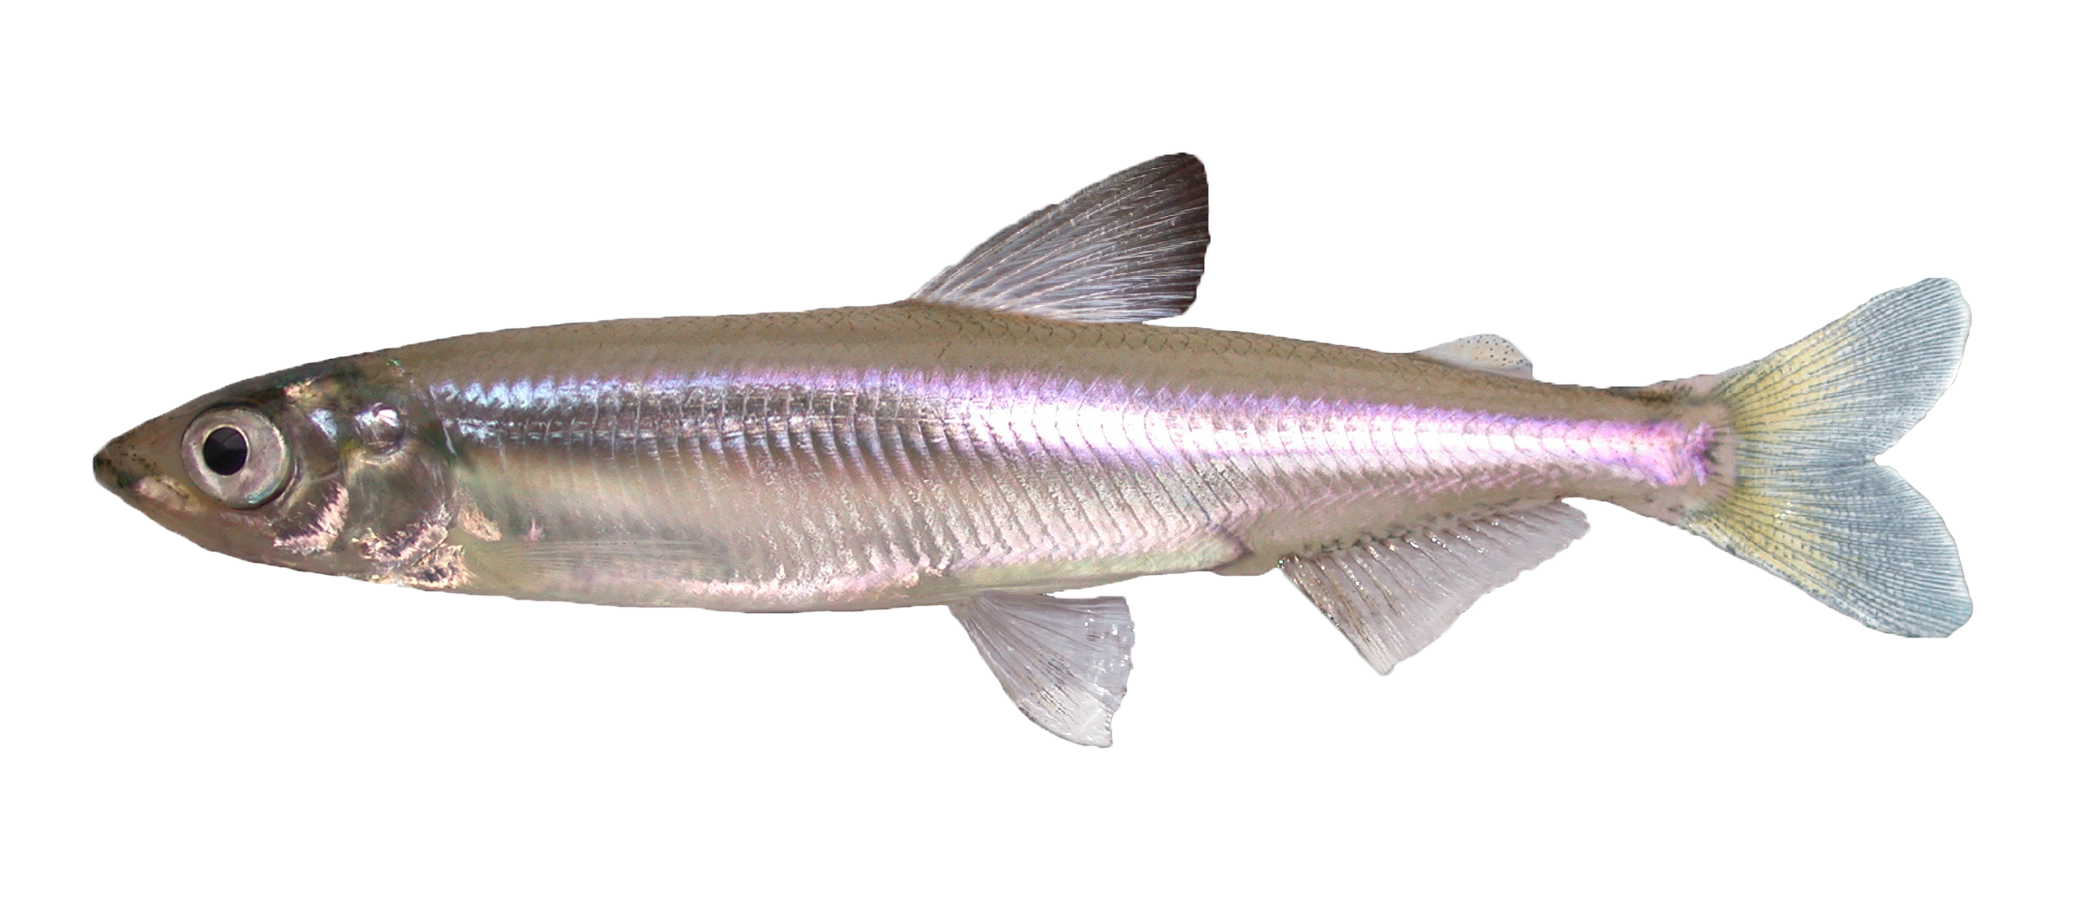
\includegraphics[width=29.17in]{figures/delta_smelt} 

}

\caption{picture of delta smelt}\label{fig:unnamed-chunk-40}
\end{figure}

\end{column800}

\begin{column40}

~

\end{column40}

\begin{column800}

\begin{figure}

{\centering 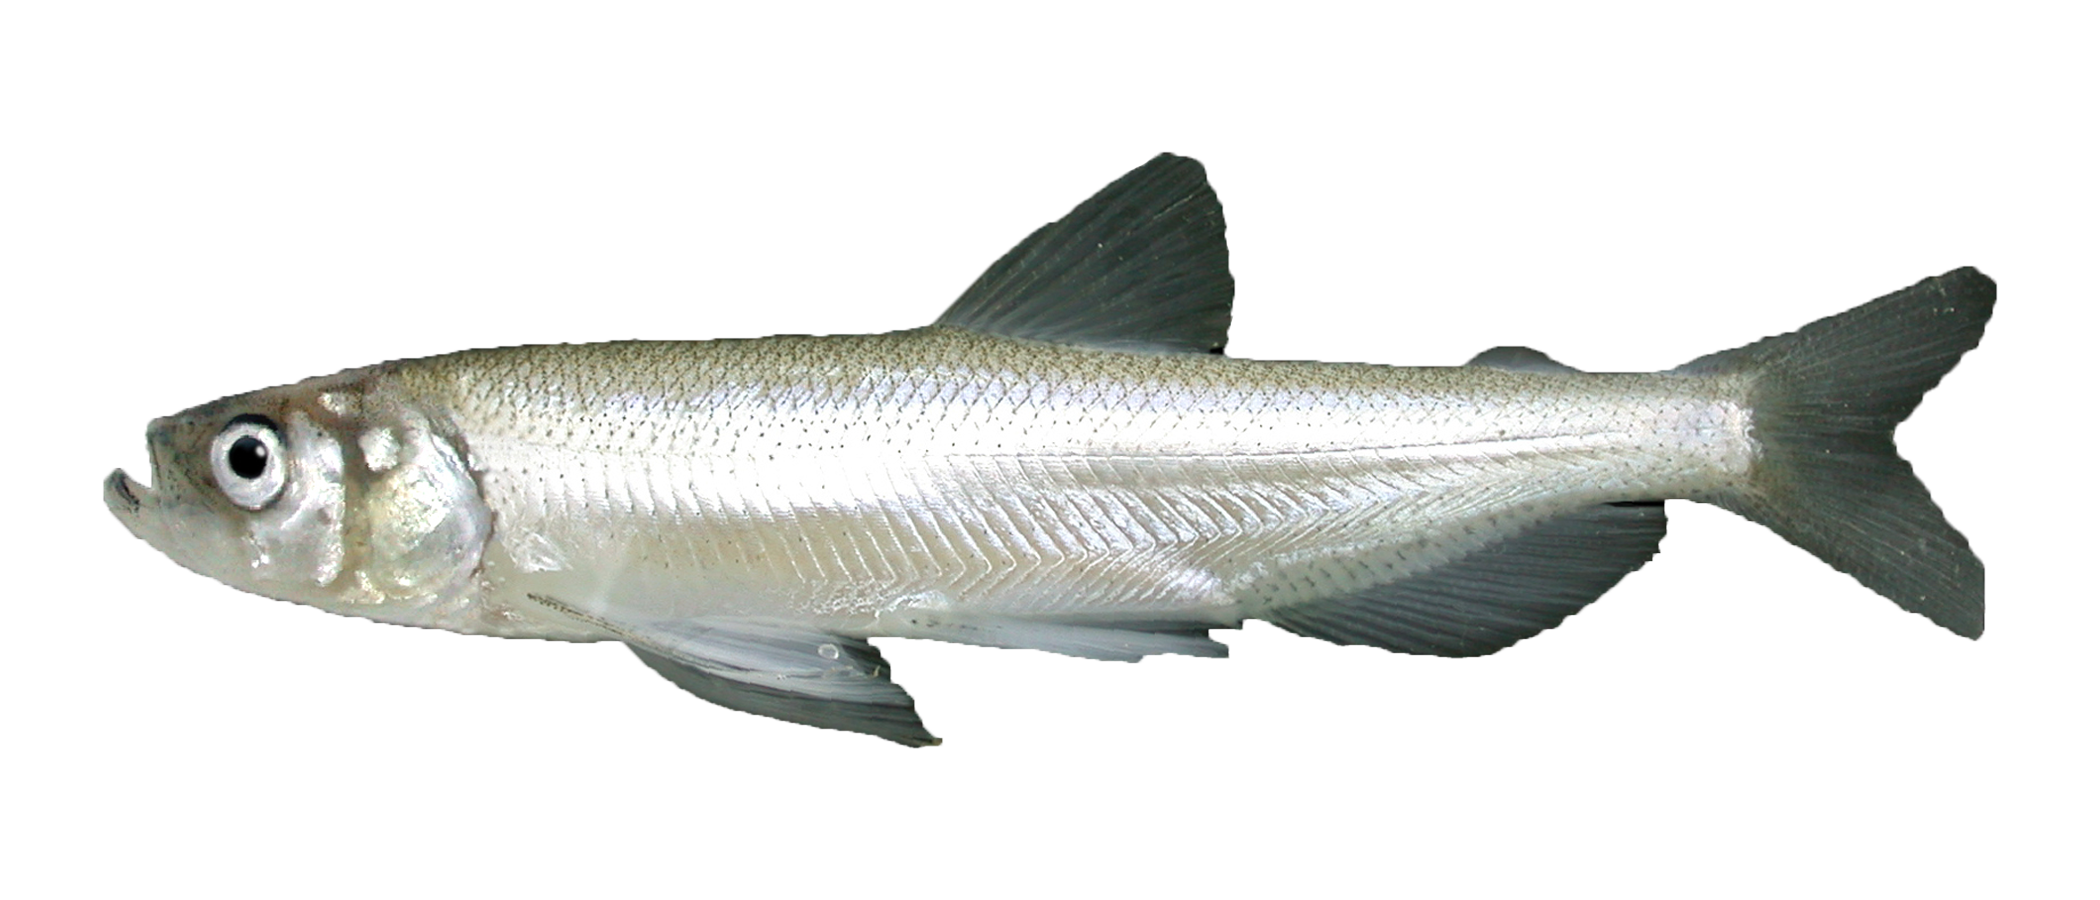
\includegraphics[width=29.17in]{figures/longfin_smelt_adult} 

}

\caption{picture of longfin smelt}\label{fig:unnamed-chunk-41}
\end{figure}

\end{column800}

\begin{column40}

~

\end{column40}

\begin{column800}

\begin{figure}

{\centering 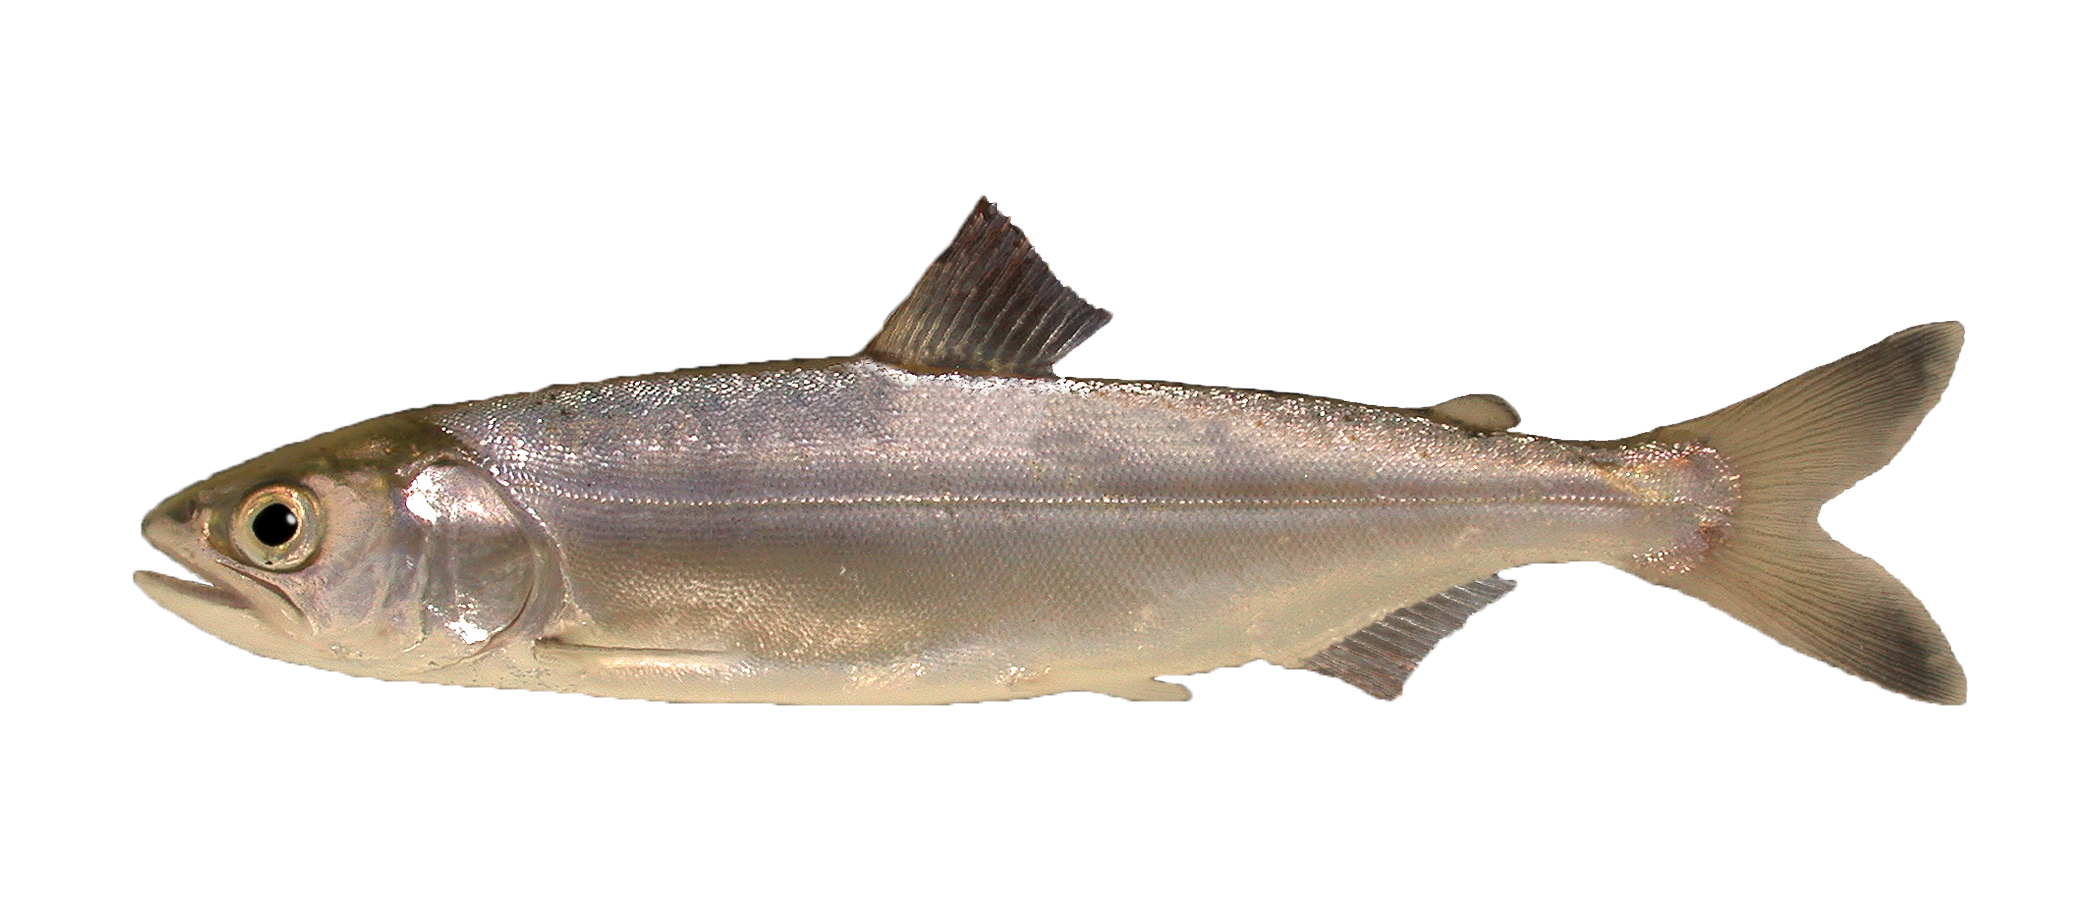
\includegraphics[width=29.17in]{figures/chinook_salmon_smolt} 

}

\caption{picture of a juvenile salmon}\label{fig:unnamed-chunk-42}
\end{figure}

\end{column800}

\end{columns-nocenter}

\begin{columns-nocenter}

\begin{column800}

\begin{expand}

\begin{figure}
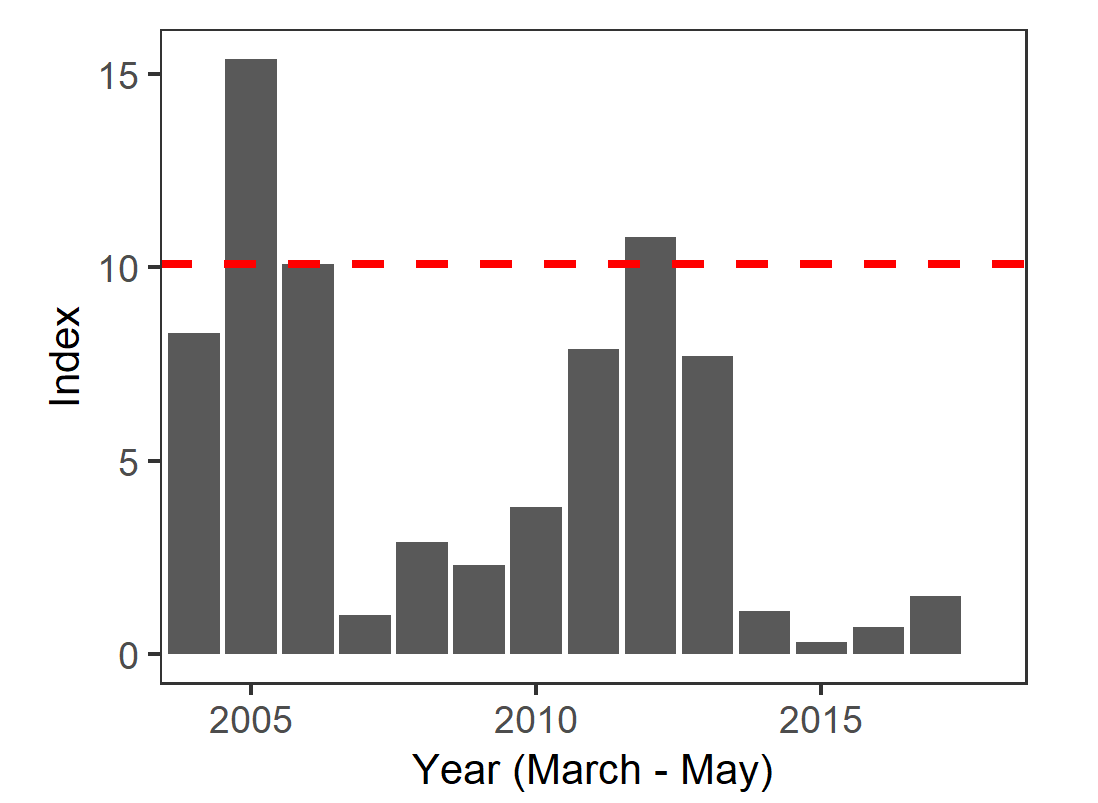
\includegraphics[width=15.25in]{figures/20mm_DSM_recent} \caption{Graph of post-larval Delta Smelt index from 2004-2018. Values range from 0 to 15.}\label{fig:unnamed-chunk-43}
\end{figure}

\end{expand}

\end{column800}

\begin{column40}

~

\end{column40}

\begin{column800}

\begin{expand}

\begin{figure}
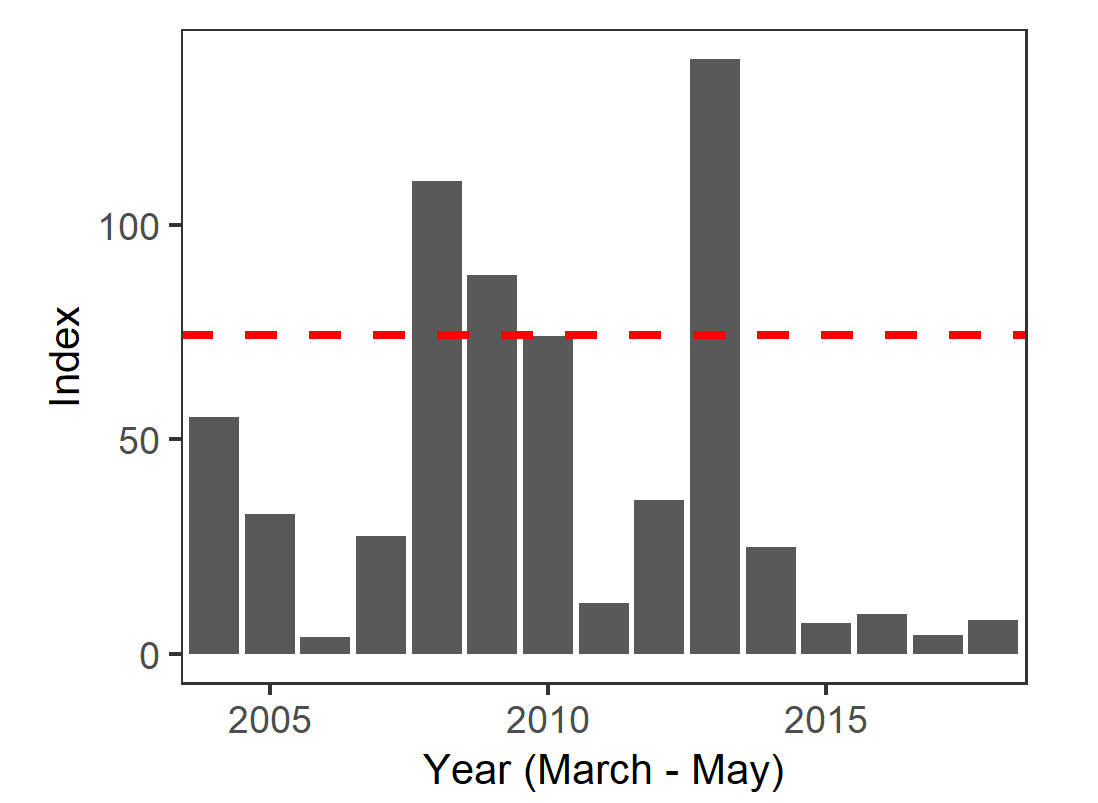
\includegraphics[width=15.25in]{figures/20mm_LFS_recent} \caption{Graph of post-larval longfin smelt index from 2004-2018. Values range from 4 to 206.}\label{fig:unnamed-chunk-44}
\end{figure}

\end{expand}

\end{column800}

\begin{column40}

~

\end{column40}

\begin{column800}

\begin{expand}

\begin{figure}
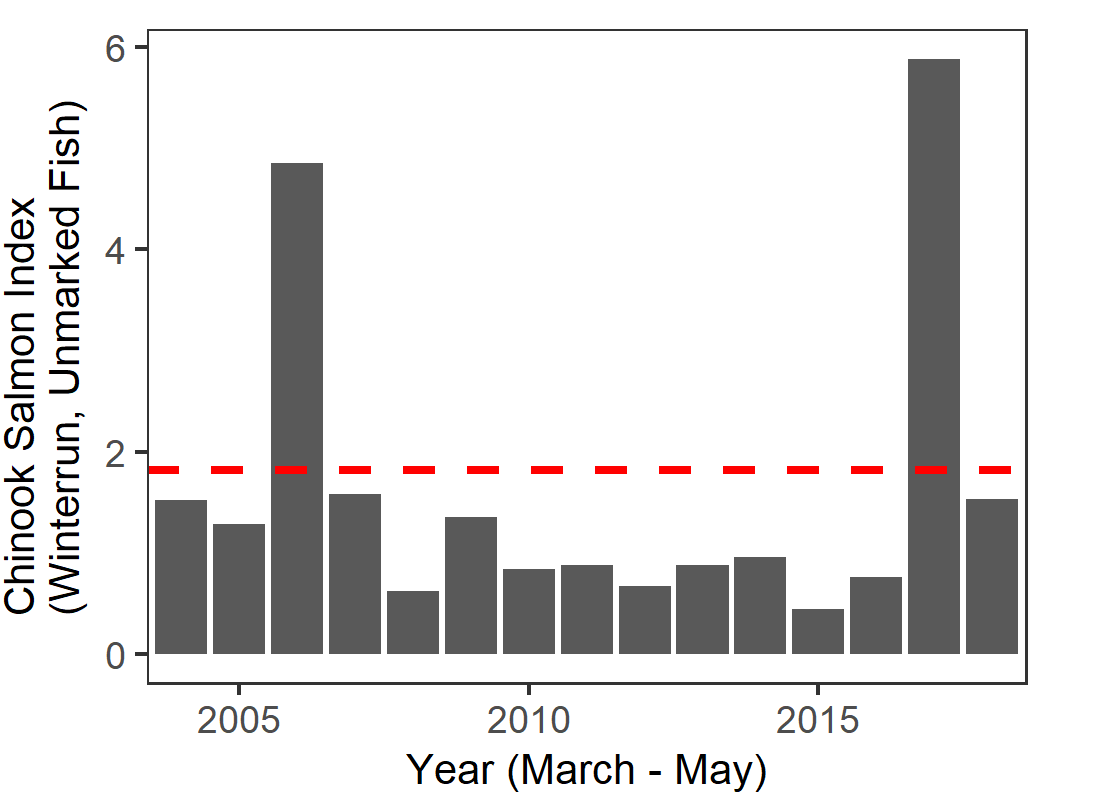
\includegraphics[width=15.25in]{figures/DJFMP_chinook_winterByLength_recyears} \caption{Graph of juvenile winter-run chinook index from 2004 to 2018. Values range from 0.2 to 6.}\label{fig:unnamed-chunk-45}
\end{figure}

\end{expand}

\end{column800}

\end{columns-nocenter}

\begin{columns-nocenter}

\begin{column800}

The Delta Smelt 20mm index was zero in 2018, the lowest index on record.

\end{column800}

\begin{column40}

~

\end{column40}

\begin{column800}

Adult Longfin smelt catch in 2018 was much lower than the long-term average.

\end{column800}

\begin{column40}

~

\end{column40}

\begin{column800}

In 2018, juvenile winter-run salmon survival was about average.

\end{column800}

\end{columns-nocenter}

\end{panel-grid}

\begin{disclaimer}
Johnson, R., S. Windell, P. L. Brandes, J. L. Conrad, J. Ferguson, P. A.
L. Goertler, B. N. Harvey, J. Heublein, J. A. Israel, D. W. Kratville,
J. E. Kirsch, R. W. Perry, J. Pisciooto, W. R. Poytress, K. Reece, and
B. G. Swart. 2017. Science Advancements Key to Increasing Management
Value of Life Stage Monitoring Networks for Endangered Sacramento River
Winter-Run Chinook Salmon in California. San Francisco Estuary and
Watershed Science 15(3). \url{https://escholarship.org/uc/item/6751j957}
\end{disclaimer}

\hypertarget{Summer}{%
\chapter{Summer Report}\label{Summer}}

\hypertarget{interagency-ecological-program-summer-season-report}{%
\subsubsection{Interagency Ecological Program Summer Season Report}\label{interagency-ecological-program-summer-season-report}}

This report shows trends in water quality, plankton, and fish across multiple IEP
surveys for June through August from 1966 to 2018.

Delta Outflow

\begin{figure}

\includegraphics[width=15.25in]{figures/mline} \caption{mean is represented by a dotted red line}\label{fig:unnamed-chunk-47}
\end{figure}

\begin{figure}
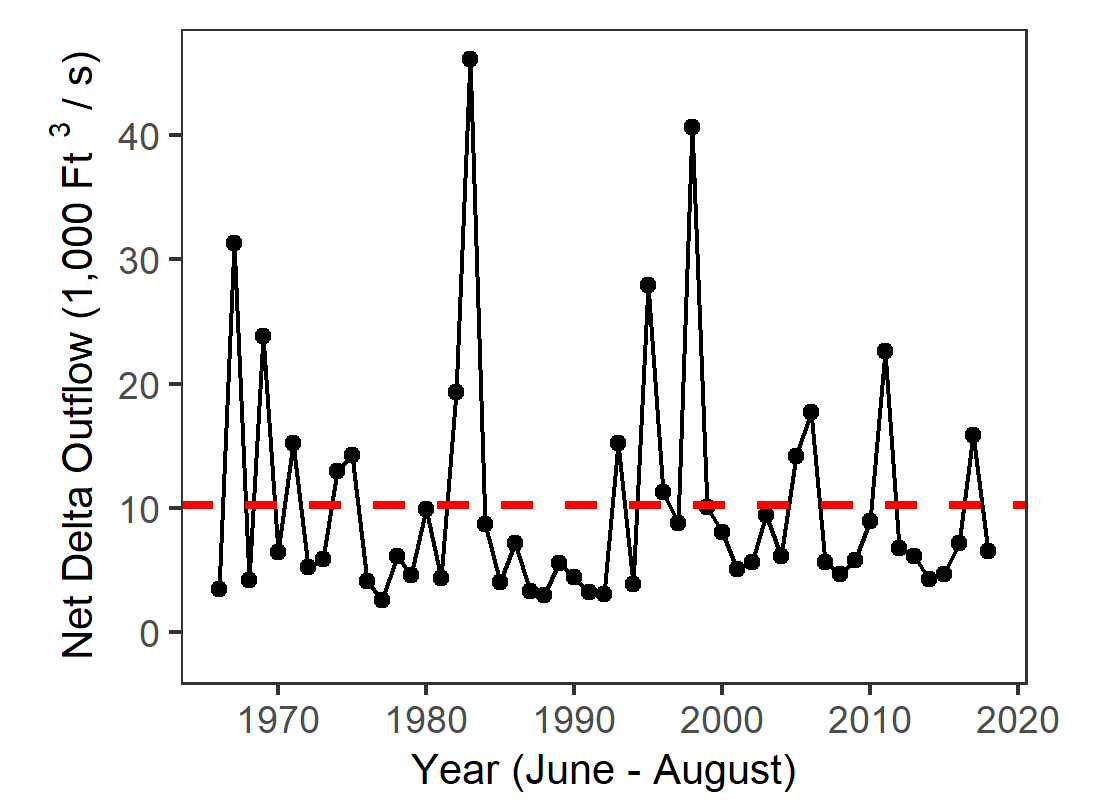
\includegraphics[width=15.25in]{figures/summer_outflow_update} \caption{average summer Delta outflow}\label{fig:unnamed-chunk-48}
\end{figure}

\begin{itemize}
\tightlist
\item
  Freshwater flow influences water quality, plankton, and fish populations.
\item
  Summer flow is driven primarily upstream dam releases and exports.
\item
  The summer of 2018 had somewhat slightly lower outflow than average.
\end{itemize}

\begin{center}\rule{0.5\linewidth}{0.5pt}\end{center}

\hypertarget{summer-secchi-depth}{%
\section{Summer Secchi Depth}\label{summer-secchi-depth}}

\begin{columns-nocenter}

\begin{column}

\hypertarget{background}{%
\subsection{Background}\label{background}}

\begin{itemize}
\tightlist
\item
  Organisms in this ecosystem are adapted to high turbidity conditions, and reductions in turbidity can have many negative ecological effects.
\item
  Higher values for Secchi depth indicate lower turbidity.
\item
  Secchi depth is measured monthly by DWR's \href{https://emp.baydeltalive.com/wiki/12297}{Environmental Monitoring Program} by dropping a black-and-white disk in the water until it disappears.
\end{itemize}

\end{column}

\begin{column}

\begin{figure}

{\centering 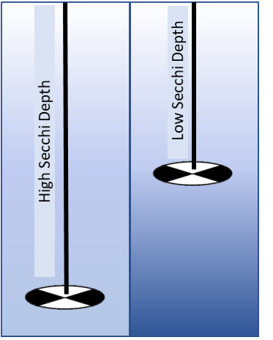
\includegraphics[width=3.79in]{figures/secchidisc} 

}

\caption{image of a secchi disk}\label{fig:unnamed-chunk-49}
\end{figure}

\end{column}

\end{columns-nocenter}

\hypertarget{average-secchi-depth-by-region}{%
\subsection{Average Secchi Depth by Region}\label{average-secchi-depth-by-region}}

\begin{columns-nocenter}

\begin{column}

\begin{figure}

\includegraphics[width=15.25in]{figures/mline} \caption{mean is represented by a dotted red line}\label{fig:unnamed-chunk-50}
\end{figure}

\end{column}

\begin{column}

\end{column}

\begin{column}

\end{column}

\end{columns-nocenter}

\begin{panel-grid}

\begin{columns-nocenter}

\begin{column800}

\textbf{San Pablo Bay}

\end{column800}

\begin{column40}

~

\end{column40}

\begin{column800}

\textbf{Suisun}

\end{column800}

\begin{column40}

~

\end{column40}

\begin{column800}

\textbf{Delta}

\end{column800}

\end{columns-nocenter}

\begin{columns-nocenter}

\begin{column800}

\begin{expand}

\begin{figure}
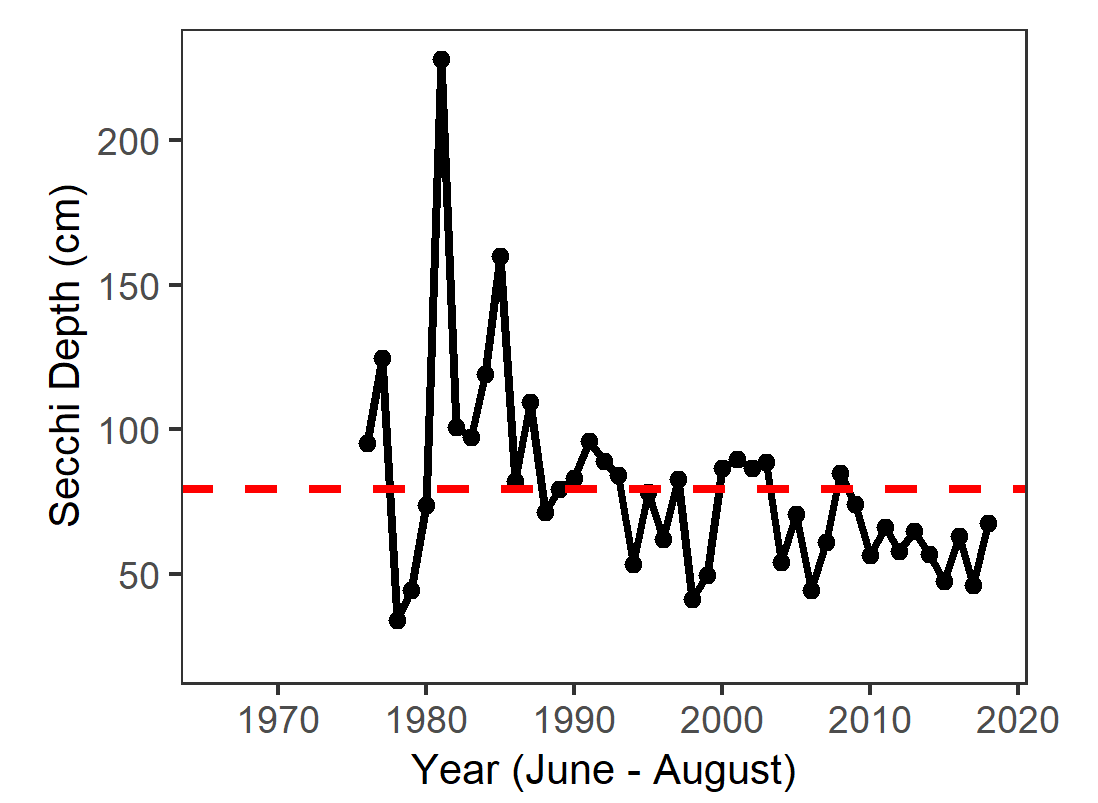
\includegraphics[width=15.25in]{figures/secchi_splsummer} \caption{Graph of average summer secchi depth in San Pablo Bay from 1975 to 2018. Values range from 10 to 150.}\label{fig:unnamed-chunk-51}
\end{figure}

\end{expand}

\end{column800}

\begin{column40}

~

\end{column40}

\begin{column800}

\begin{expand}

\begin{figure}
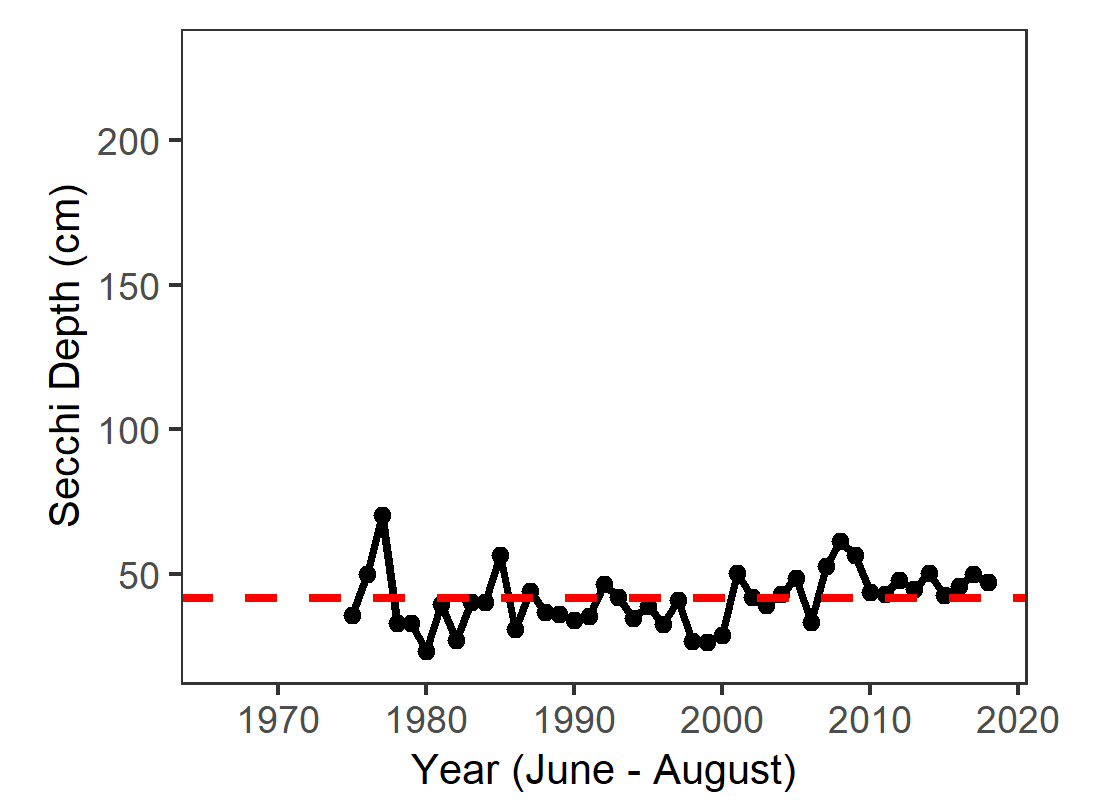
\includegraphics[width=15.25in]{figures/secchi_sssummer} \caption{Graph of average summer secchi depth in Suisun from 1975 to 2018. Values range from 10 to 60.}\label{fig:unnamed-chunk-52}
\end{figure}

\end{expand}

\end{column800}

\begin{column40}

~

\end{column40}

\begin{column800}

\begin{expand}

\begin{figure}
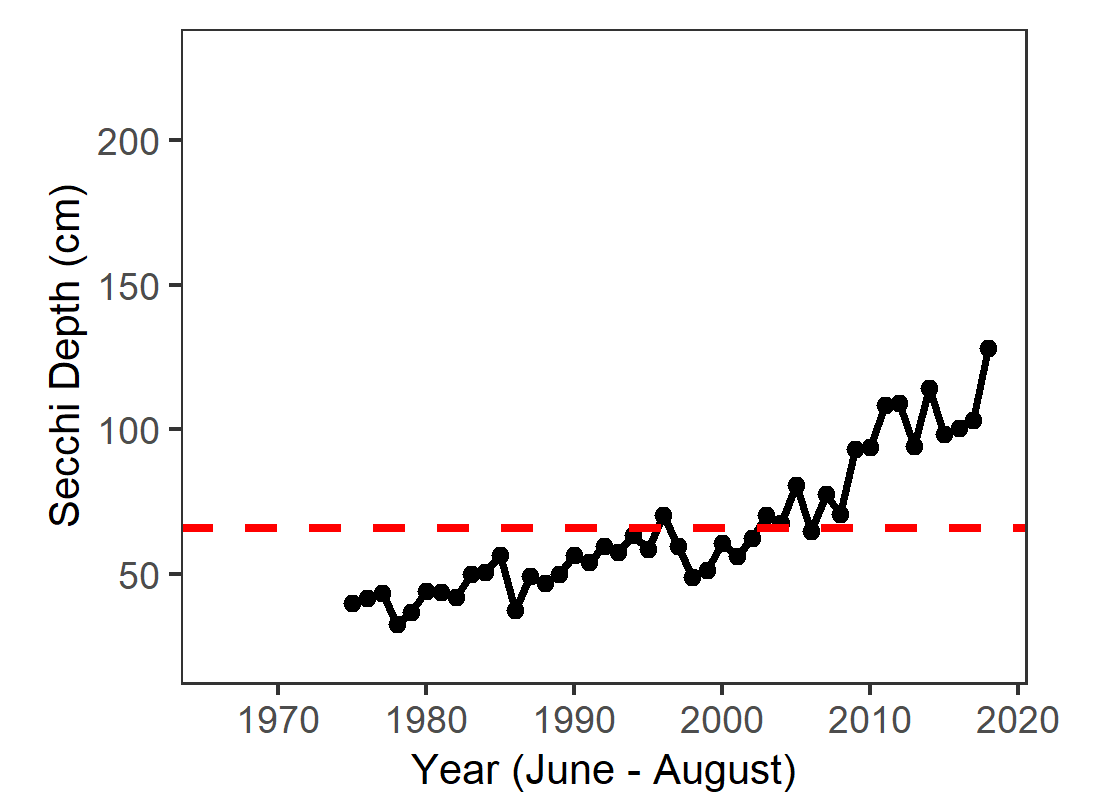
\includegraphics[width=15.25in]{figures/secchi_dtsummer} \caption{Graph of average summer secchi depth in the Delta from 1975 to 2018. Values range from 25 to 120 and have been increasing since the year 2000.}\label{fig:unnamed-chunk-53}
\end{figure}

\end{expand}

\end{column800}

\end{columns-nocenter}

\begin{columns-nocenter}

\begin{column800}

In 2018, San Pablo bay was close to the long-term average.

\end{column800}

\begin{column40}

~

\end{column40}

\begin{column800}

In 2018, Suisun Bay was also close to the long-term average.

\end{column800}

\begin{column40}

~

\end{column40}

\begin{column800}

In 2018, the Delta was much clearer than average, the clearest summer on record.

\end{column800}

\end{columns-nocenter}

\end{panel-grid}

\begin{disclaimer}
For more information see:
\href{https://link.springer.com/article/10.1007/s12237-011-9382-x}{Schoellhamer,
D. H. 2011. Sudden clearing of estuarine waters upon crossing the
threshold from transport to supply regulation of sediment transport as
an erodible sediment pool is depleted: San Francisco Bay, 1999.
Estuaries and Coasts 34(5):885-899.}
\end{disclaimer}

\begin{center}\rule{0.5\linewidth}{0.5pt}\end{center}

\hypertarget{summer-water-temperature}{%
\section{Summer Water Temperature}\label{summer-water-temperature}}

\begin{columns-nocenter}

\begin{column}

\hypertarget{background-1}{%
\subsection{Background}\label{background-1}}

\begin{itemize}
\tightlist
\item
  Water temperature is monitored monthly by DWR's \href{https://emp.baydeltalive.com/wiki/12297}{Environmental Monitoring Program}.
\item
  High temperature can increase productivity and may trigger harmful algal blooms.
\item
  Increasing Summer temperatures may limit juvenile smelt survival.
\item
  Summer temperatures are lower closer to the ocean and slightly higher in the Delta.
\end{itemize}

\end{column}

\begin{column}

\begin{figure}

{\centering 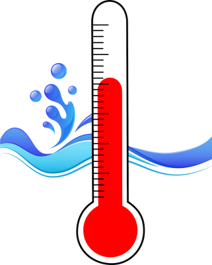
\includegraphics[width=2.94in]{figures/thermometer} 

}

\caption{picture of a thermometer in water}\label{fig:unnamed-chunk-55}
\end{figure}

\end{column}

\end{columns-nocenter}

\hypertarget{average-temperature-by-region}{%
\subsection{Average Temperature by Region}\label{average-temperature-by-region}}

\begin{columns-nocenter}

\begin{column}

\begin{figure}

\includegraphics[width=15.25in]{figures/mline} \caption{mean is represented by a dotted red line}\label{fig:unnamed-chunk-56}
\end{figure}

\end{column}

\begin{column}

\end{column}

\begin{column}

\end{column}

\end{columns-nocenter}

\begin{panel-grid}

\begin{columns-nocenter}

\begin{column800}

\textbf{San Pablo Bay}

\end{column800}

\begin{column40}

~

\end{column40}

\begin{column800}

\textbf{Suisun}

\end{column800}

\begin{column40}

~

\end{column40}

\begin{column800}

\textbf{Delta}

\end{column800}

\end{columns-nocenter}

\begin{columns-nocenter}

\begin{column800}

\begin{expand}

\begin{figure}
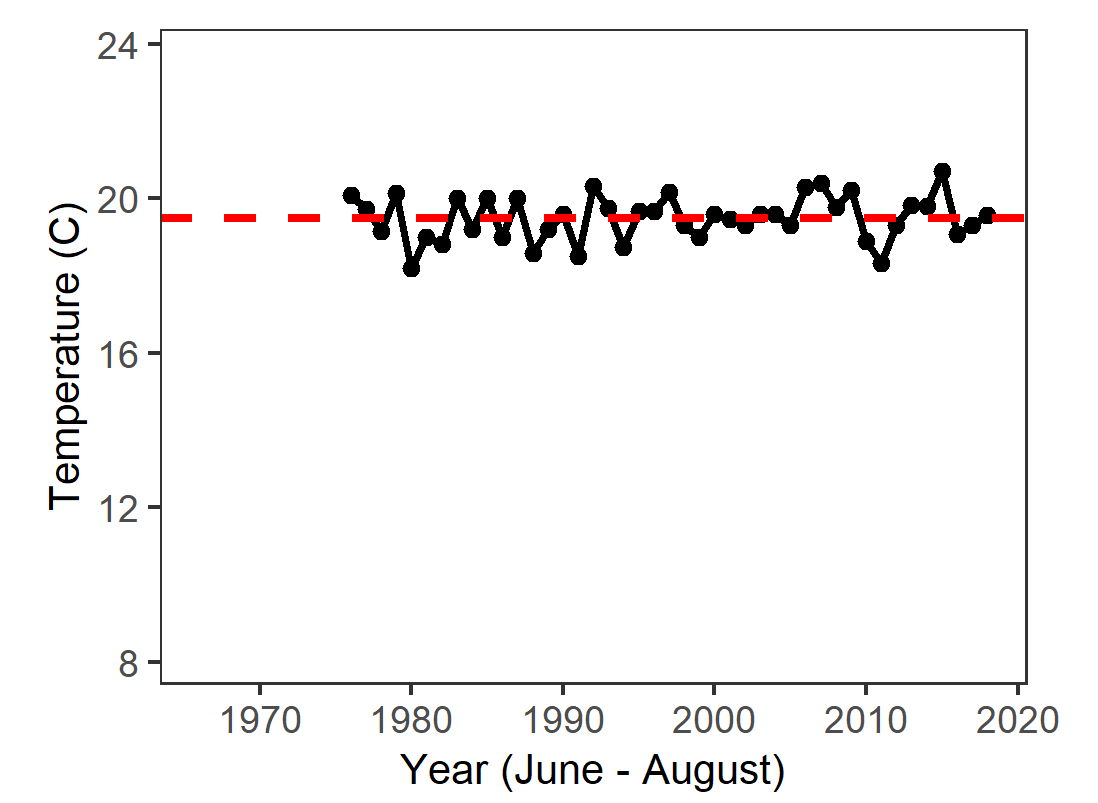
\includegraphics[width=15.25in]{figures/temp_splsummer} \caption{Graph of average summer water temperature in San Pablo Bay from 1975 to 2018. Values range from 13 to 18.}\label{fig:unnamed-chunk-57}
\end{figure}

\end{expand}

\end{column800}

\begin{column40}

~

\end{column40}

\begin{column800}

\begin{expand}

\begin{figure}
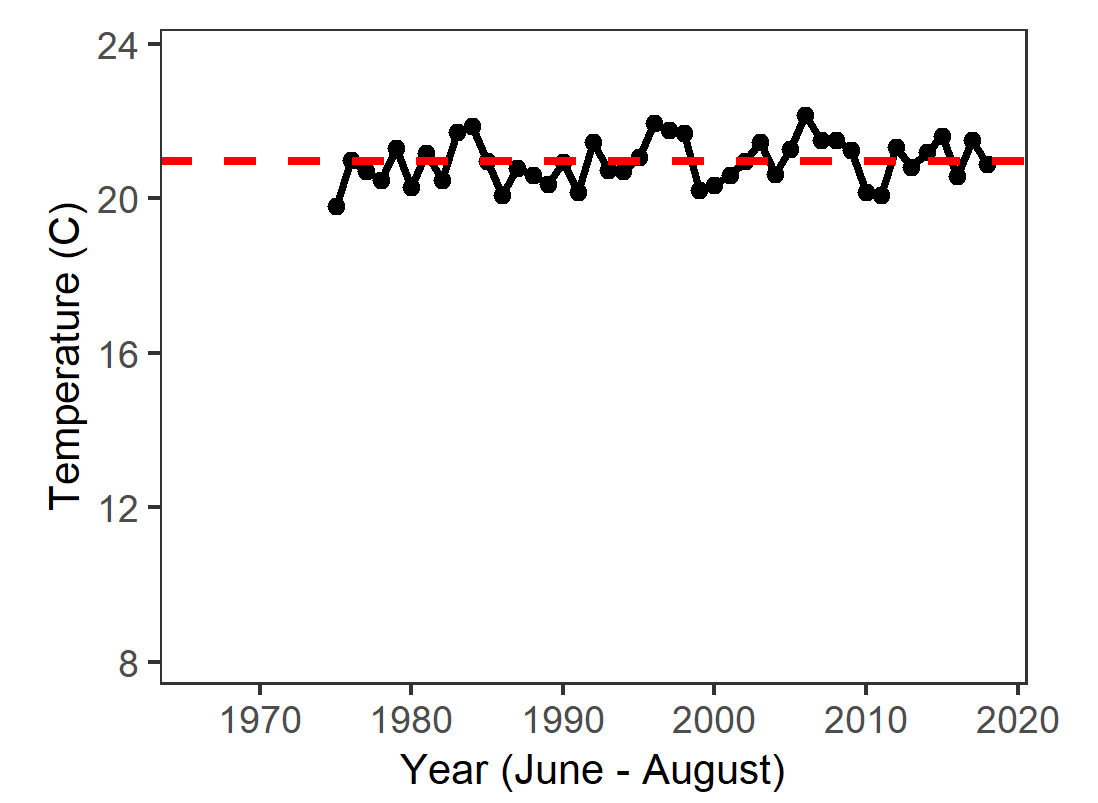
\includegraphics[width=15.25in]{figures/temp_sssummer} \caption{Graph of average summer water temperature in Suisun from 1975 to 2018. Values range from 13 to 18.}\label{fig:unnamed-chunk-58}
\end{figure}

\end{expand}

\end{column800}

\begin{column40}

~

\end{column40}

\begin{column800}

\begin{expand}

\begin{figure}
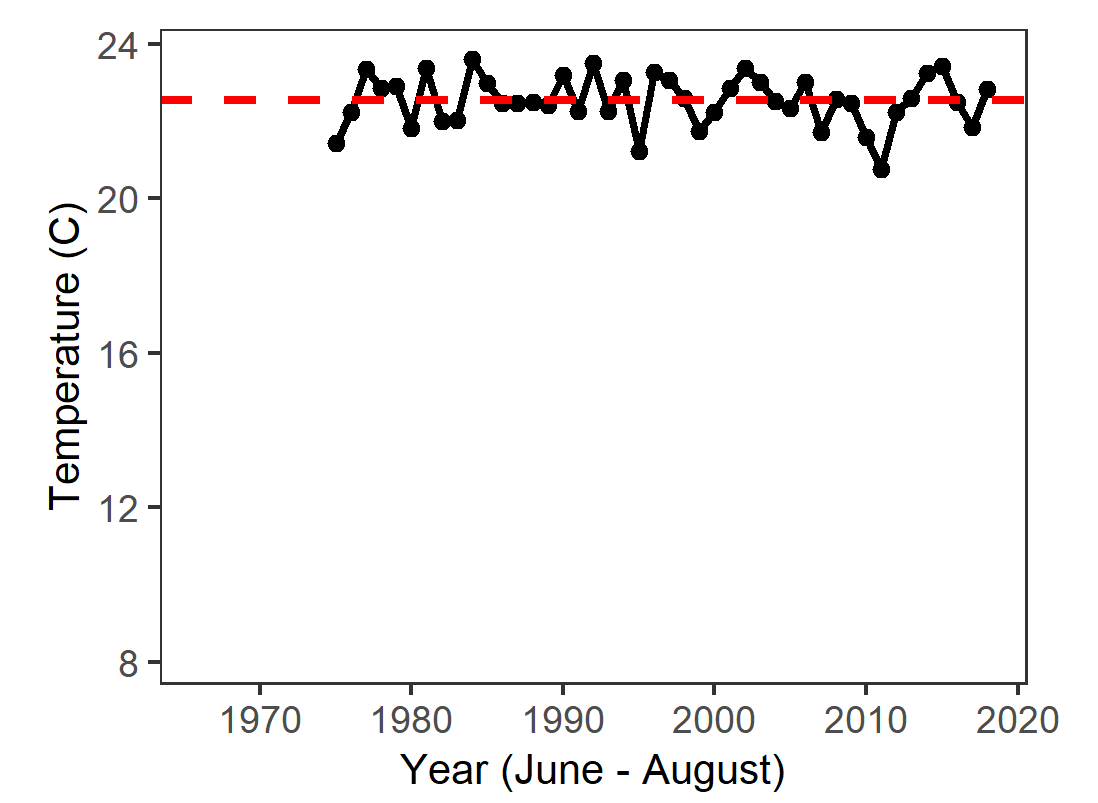
\includegraphics[width=15.25in]{figures/temp_dtsummer} \caption{Graph of average summer water temperature in the Delta from 1975 to 2018. Values range from 13 to 18.}\label{fig:unnamed-chunk-59}
\end{figure}

\end{expand}

\end{column800}

\end{columns-nocenter}

\begin{columns-nocenter}

\begin{column800}

In 2018, San Pablo Bay temperatures were similar to the long-term average.

\end{column800}

\begin{column40}

~

\end{column40}

\begin{column800}

In 2018, Suisun Bay was similar to the long-term average.

\end{column800}

\begin{column40}

~

\end{column40}

\begin{column800}

In 2018, the Delta was slightly cooler than average.

\end{column800}

\end{columns-nocenter}

\end{panel-grid}

\begin{disclaimer}
For more information see:
\href{https://www.sciencedirect.com/science/article/pii/S1568988316302177}{Lehman,
P. W., T. Kurobe, S. Lesmeister, D. Baxa, A. Tung, and S. J. Teh. 2017.
Impacts of the 2014 severe drought on the Microcystis bloom in San
Francisco Estuary. Harmful Algae 63(Supplement C):94-108.}
\end{disclaimer}

\begin{center}\rule{0.5\linewidth}{0.5pt}\end{center}

\hypertarget{summer-chlorophyll}{%
\section{Summer Chlorophyll}\label{summer-chlorophyll}}

\begin{columns-nocenter}

\begin{column}

\hypertarget{background-2}{%
\subsection{Background}\label{background-2}}

\begin{itemize}
\tightlist
\item
  Chlorophyll is an indicator of phytoplankton production, which is low during the summer.
\item
  Phytoplankton are the base of the pelagic food web. It is sampled monthly by DWR's \href{https://emp.baydeltalive.com/wiki/12297}{Environmental Monitoring Program}.
\item
  The invasion of the clam \emph{Potamocorbula amurensis} caused a decline in phytoplankton and zooplankton after 1986 -- especially in Suisun Bay.
\end{itemize}

\end{column}

\begin{column}

\begin{figure}

{\centering \includegraphics[width=2.57in]{figures/phyto} 

}

\caption{picture of phytoplankton}\label{fig:unnamed-chunk-61}
\end{figure}

\end{column}

\end{columns-nocenter}

\hypertarget{average-chlorophyll-by-region}{%
\subsection{Average Chlorophyll by Region}\label{average-chlorophyll-by-region}}

\begin{columns-nocenter}

\begin{column}

\begin{figure}
\includegraphics[width=15.25in]{figures/mline} \caption{mean is represented by a dotted red line}\label{fig:unnamed-chunk-62}
\end{figure}

\end{column}

\begin{column}

\end{column}

\begin{column}

\end{column}

\end{columns-nocenter}

\begin{panel-grid}

\begin{columns-nocenter}

\begin{column800}

\textbf{San Pablo Bay}

\end{column800}

\begin{column40}

~

\end{column40}

\begin{column800}

\textbf{Suisun}

\end{column800}

\begin{column40}

~

\end{column40}

\begin{column800}

\textbf{Delta}

\end{column800}

\end{columns-nocenter}

\begin{columns-nocenter}

\begin{column800}

\begin{expand}

\begin{figure}
\includegraphics[width=15.25in]{figures/chla_splsummer} \caption{Graph of average summer chlorophyll in San Pablo Bay from 1975 to 2018. Values range from 4 to 15.}\label{fig:unnamed-chunk-63}
\end{figure}

\end{expand}

\end{column800}

\begin{column40}

~

\end{column40}

\begin{column800}

\begin{expand}

\begin{figure}
\includegraphics[width=15.25in]{figures/chla_sssummer} \caption{Graph of average summer chlorophyll in Suisun from 1975 to 2018. Values range from 2 to 19.}\label{fig:unnamed-chunk-64}
\end{figure}

\end{expand}

\end{column800}

\begin{column40}

~

\end{column40}

\begin{column800}

\begin{expand}

\begin{figure}
\includegraphics[width=15.25in]{figures/chla_dtsummer} \caption{Graph of average summer chlorophyll in the Delta from 1975 to 2018. Values range from 3.5 to 29.}\label{fig:unnamed-chunk-65}
\end{figure}

\end{expand}

\end{column800}

\end{columns-nocenter}

\begin{columns-nocenter}

\begin{column800}

In 2018, San Pablo Bay chlorophyll was similar to the long-term average.

\end{column800}

\begin{column40}

~

\end{column40}

\begin{column800}

In 2018, Suisun Bay chlorophyll was below average.

\end{column800}

\begin{column40}

~

\end{column40}

\begin{column800}

In 2018, the Delta had lower chlorophyll than average.

\end{column800}

\end{columns-nocenter}

\end{panel-grid}

\begin{disclaimer}
For more information see: Cahoon, T. and T. Brown. 2018. Phytoplankton,
Chlorophyll-a and Pheophytin-a Status and Trends 2017. IEP Newsletter
32(1):14-20. Available on request:
\href{mailto:iepnewsletter@water.ca.gov}{\nolinkurl{iepnewsletter@water.ca.gov}}
\end{disclaimer}

\begin{center}\rule{0.5\linewidth}{0.5pt}\end{center}

\hypertarget{summer-zooplankton}{%
\section{Summer Zooplankton}\label{summer-zooplankton}}

\hypertarget{background-3}{%
\subsection{Background}\label{background-3}}

\begin{columns-nocenter}

\begin{column}

\begin{itemize}
\tightlist
\item
  Zooplankton is sampled monthly by the CDFW/DWR \href{https://emp.baydeltalive.com/wiki/12297}{Environmental Monitoring Program} but sampling in San Pablo Bay did not begin until 1998.
\item
  Zooplankton are an important food source for pelagic fish.
\item
  Calanoid copepods and mysids are particularly good fish food. Cyclopoid copepods are not as good for fish food.
\item
  Biomass in summer tends to be the highest of the year, particularly for the calanoid copepod \emph{Pseudodiaptomous forbesi}.
\end{itemize}

\end{column}

\begin{column}

Copepod

\begin{figure}

{\centering \includegraphics[width=16.67in]{figures/acartia} 

}

\caption{picture of a copepod}\label{fig:unnamed-chunk-67}
\end{figure}

Mysid

\begin{figure}

{\centering \includegraphics[width=16.67in]{figures/mysid} 

}

\caption{picture of a copepod}\label{fig:unnamed-chunk-68}
\end{figure}

\end{column}

\end{columns-nocenter}

\hypertarget{average-zooplankton-biomass-by-region}{%
\subsection{Average Zooplankton Biomass by Region}\label{average-zooplankton-biomass-by-region}}

\begin{columns-nocenter}

\begin{column}

\begin{figure}
\includegraphics[width=15.25in]{figures/mline} \caption{mean is represented by a dotted red line}\label{fig:unnamed-chunk-69}
\end{figure}

\end{column}

\begin{column}

\end{column}

\begin{column}

\end{column}

\end{columns-nocenter}

\begin{panel-grid}

\begin{columns-nocenter}

\begin{column800}

\textbf{San Pablo Bay}

\end{column800}

\begin{column40}

~

\end{column40}

\begin{column800}

\textbf{Suisun}

\end{column800}

\begin{column40}

~

\end{column40}

\begin{column800}

\textbf{Delta}

\end{column800}

\end{columns-nocenter}

\begin{columns-nocenter}

\begin{column800}

\begin{expand}

\begin{figure}
\includegraphics[width=15.25in]{figures/zoops_splsummer} \caption{Graph of average summer zooplankton biomass in San Pablo Bay from 1975 to 2018. Values range from 5 to 25.}\label{fig:unnamed-chunk-70}
\end{figure}

\end{expand}

\end{column800}

\begin{column40}

~

\end{column40}

\begin{column800}

\begin{expand}

\begin{figure}
\includegraphics[width=15.25in]{figures/zoops_sssummer} \caption{Graph of average summer chlorophyll in Suisun from 1975 to 2018. Values range from 5 to 45 with much higher biomass before 1986.}\label{fig:unnamed-chunk-71}
\end{figure}

\end{expand}

\end{column800}

\begin{column40}

~

\end{column40}

\begin{column800}

\begin{expand}

\begin{figure}
\includegraphics[width=15.25in]{figures/zoops_dtsummer} \caption{Graph of average summer zooplankton biomass in the Delta from 1975 to 2018. Values range from 3.5 to 39.}\label{fig:unnamed-chunk-72}
\end{figure}

\end{expand}

\end{column800}

\end{columns-nocenter}

\begin{columns-nocenter}

\begin{column800}

In 2018, San Pablo Bay had slightly higher biomass than average, mostly cyclopoid copepods.

\end{column800}

\begin{column40}

~

\end{column40}

\begin{column800}

In 2018, Suisun Bay also had slightly higher than average total biomass, mostly mysids and cylcopoid copepdos.

\end{column800}

\begin{column40}

~

\end{column40}

\begin{column800}

In 2018, the Delta had about average total biomass, mostly cladocerans.

\end{column800}

\end{columns-nocenter}

\end{panel-grid}

\begin{disclaimer}
For more information see: Hennessy, A. 2018. Zooplankton Monitoring
2018. IEP Newsletter 32(1):21-32. Available on request:
\href{mailto:iepnewsletter@water.ca.gov}{\nolinkurl{iepnewsletter@water.ca.gov}}
\end{disclaimer}

\begin{center}\rule{0.5\linewidth}{0.5pt}\end{center}

\hypertarget{summer-fish}{%
\section{Summer Fish}\label{summer-fish}}

\hypertarget{background-4}{%
\subsection{Background}\label{background-4}}

\begin{itemize}
\tightlist
\item
  Delta Smelt, listed as threatened by the Endangered Species Act, have been tracked by \href{https://wildlife.ca.gov/Conservation/Delta/Townet-Survey}{CDFW's Townet Survey} since 1959 in Suisun Bay, San Pablo Bay, and the Delta.
\item
  Northern Anchovy are an important forage fish in the brackish-saline regions of the estuary. They are sampled best by \href{https://wildlife.ca.gov/Conservation/Delta/Bay-Study}{CDFW's San Francisco Bay Study}.
\item
  Sacramento Pikeminnow is a native cyprinid that is one of the few piscivorous native fish in the Delta. They are sampled by \href{https://www.fws.gov/lodi/juvenile_fish_monitoring_program/jfmp_index.htm}{USFWS's DJFMP} beach seine surveys throughout the estuary.
\end{itemize}

\hypertarget{average-fish-catch-trends-by-species}{%
\subsection{Average Fish Catch Trends by Species}\label{average-fish-catch-trends-by-species}}

\begin{columns-nocenter}

\begin{column}

\begin{figure}
\includegraphics[width=15.25in]{figures/mline} \caption{mean is represented by a dotted red line}\label{fig:unnamed-chunk-74}
\end{figure}

\end{column}

\begin{column}

\begin{figure}
\includegraphics[width=15.25in]{figures/mpoint} \caption{missing data are represented by tan triangles}\label{fig:unnamed-chunk-75}
\end{figure}

\end{column}

\begin{column}

\end{column}

\end{columns-nocenter}

\begin{panel-grid}

\begin{columns-nocenter}

\begin{column800}

\textbf{Delta Smelt}

\end{column800}

\begin{column40}

~

\end{column40}

\begin{column800}

\textbf{Northern Anchovy}

\end{column800}

\begin{column40}

~

\end{column40}

\begin{column800}

\textbf{Sacramento Pikeminnow}

\end{column800}

\end{columns-nocenter}

\begin{columns-nocenter}

\begin{column800}

\begin{figure}

{\centering \includegraphics[width=29.17in]{figures/delta_smelt} 

}

\caption{picture of a delta smelt}\label{fig:unnamed-chunk-76}
\end{figure}

\end{column800}

\begin{column40}

~

\end{column40}

\begin{column800}

\begin{figure}

{\centering \includegraphics[width=14.58in]{figures/Anchovy-1} 

}

\caption{picture of a northern anchovy}\label{fig:unnamed-chunk-77}
\end{figure}

\end{column800}

\begin{column40}

~

\end{column40}

\begin{column800}

\begin{figure}

{\centering \includegraphics[width=29.17in]{figures/sacramento_pikeminnow} 

}

\caption{picture of a sacramento pikeminnow}\label{fig:unnamed-chunk-78}
\end{figure}

\end{column800}

\end{columns-nocenter}

\begin{columns-nocenter}

\begin{column800}

\begin{expand}

\begin{figure}
\includegraphics[width=15.25in]{figures/STN_DSM} \caption{Graph of Delta Smelt Index from 1970 to 2018. Values range from 0 to 62.}\label{fig:unnamed-chunk-79}
\end{figure}

\end{expand}

\end{column800}

\begin{column40}

~

\end{column40}

\begin{column800}

\begin{expand}

\begin{figure}
\includegraphics[width=15.25in]{figures/noranc_all_years} \caption{Graph of average northern anchovy CPUE from 1980 through 2017.}\label{fig:unnamed-chunk-80}
\end{figure}

\end{expand}

\end{column800}

\begin{column40}

~

\end{column40}

\begin{column800}

\begin{expand}

\begin{figure}
\includegraphics[width=15.25in]{figures/DJFMP_sacpikeminnow_summer} \caption{Graph of Sacramento pikeminnow index from 1975 to 2018. Values range from 0.2 to 6.}\label{fig:unnamed-chunk-81}
\end{figure}

\end{expand}

\end{column800}

\end{columns-nocenter}

\begin{columns-nocenter}

\begin{column800}

Delta Smelt catch in 2018 was much lower than the longterm average.

\end{column800}

\begin{column40}

~

\end{column40}

\begin{column800}

Bay Study has not been able to complete their surveys in recent years, but the most recent complete survey was about average.

\end{column800}

\begin{column40}

~

\end{column40}

\begin{column800}

In 2018, Pikeminnow were less abundant than average.

\end{column800}

\end{columns-nocenter}

\end{panel-grid}

\begin{disclaimer}
For more information see: Hieb, K., J. Bautista, and J. Giannetta. 2018.
Bay Study Fishes Status and Trends Report for the San Francisco Estuary,
2012--2016. IEP Newsletter 31(2):3-43. Available on request:
\href{mailto:iepnewsletter@water.ca.gov}{\nolinkurl{iepnewsletter@water.ca.gov}}
\end{disclaimer}

\begin{center}\rule{0.5\linewidth}{0.5pt}\end{center}

\hypertarget{recent-trends-summer-2004-2018}{%
\section{Recent Trends: Summer 2004-2018}\label{recent-trends-summer-2004-2018}}

\hypertarget{background-5}{%
\subsection{Background}\label{background-5}}

\begin{itemize}
\tightlist
\item
  Delta Smelt have been in severe decline over the past two decades, with a \href{https://wildlife.ca.gov/Conservation/Delta/Townet-Survey}{Summer Townet Survey} index of zero in 2015, 2016 and 2018.
\item
  \emph{Microcystis} is a toxic cyanobacteria first found in the Delta in 1998. \emph{Microcystis} presence has been documented by the \href{https://emp.baydeltalive.com/wiki/12297}{Environmental Monitoring Program} and the \href{https://wildlife.ca.gov/Conservation/Delta/Townet-Survey}{CDFW Summer Townet Survey} during their water quality sampling.
\item
  Aquatic vegetation in the Delta has increased significantly in recent years. This vegetation is composed mostly of non-native invasive plant species and is categorized as either floating or submerged types. Coverage is estimated by \href{http://cstars.metro.ucdavis.edu/}{UC-Davis} using remote sensing of the North and Central Delta.
\end{itemize}

\hypertarget{average-trends-by-parameter}{%
\subsection{Average Trends by Parameter}\label{average-trends-by-parameter}}

\begin{columns-nocenter}

\begin{column}

\begin{figure}
\includegraphics[width=15.25in]{figures/mline} \caption{mean is represented by a dotted red line}\label{fig:unnamed-chunk-83}
\end{figure}

\end{column}

\begin{column}

\begin{figure}
\includegraphics[width=15.25in]{figures/mpoint} \caption{missing data are represented by tan triangles}\label{fig:unnamed-chunk-84}
\end{figure}

\end{column}

\begin{column}

\end{column}

\end{columns-nocenter}

\begin{panel-grid}

\begin{columns-nocenter}

\begin{column800}

\textbf{Delta Smelt}

\end{column800}

\begin{column40}

~

\end{column40}

\begin{column800}

\textbf{Microcystis}

\end{column800}

\begin{column40}

~

\end{column40}

\begin{column800}

\textbf{Invasive Aquatic Vegetation}

\end{column800}

\end{columns-nocenter}

\begin{columns-nocenter}

\begin{column800}

\begin{figure}

{\centering \includegraphics[width=29.17in]{figures/delta_smelt} 

}

\caption{picture of delta smelt}\label{fig:unnamed-chunk-85}
\end{figure}

\end{column800}

\begin{column40}

~

\end{column40}

\begin{column800}

\begin{figure}

{\centering \includegraphics{figures/microcystis} 

}

\caption{picture of a beaker with flakes of microcystis floating in it}\label{fig:unnamed-chunk-86}
\end{figure}

\end{column800}

\begin{column40}

~

\end{column40}

\begin{column800}

\begin{figure}

{\centering \includegraphics[width=4.74in]{figures/egeria} 

}

\caption{picture of a beaker with flakes of microcystis floating in it}\label{fig:unnamed-chunk-87}
\end{figure}

\end{column800}

\end{columns-nocenter}

\begin{columns-nocenter}

\begin{column800}

\begin{expand}

\begin{figure}
\includegraphics[width=15.25in]{figures/STN_DSM_rec} \caption{Graph of juvenile Delta Smelt index from 2004-2018. Values range from 0 to 15.}\label{fig:unnamed-chunk-88}
\end{figure}

\end{expand}

\end{column800}

\begin{column40}

~

\end{column40}

\begin{column800}

\begin{expand}

\begin{figure}
\includegraphics[width=15.25in]{figures/Microcystis_summer} \caption{Graph of microcystis abundance fron 2007 to 2018}\label{fig:unnamed-chunk-89}
\end{figure}

\end{expand}

\end{column800}

\begin{column40}

~

\end{column40}

\begin{column800}

\begin{expand}

\begin{figure}
\includegraphics[width=15.25in]{figures/veg_perc} \caption{Graph of percent coverage of submerged and floating vegetation in the Delta.}\label{fig:unnamed-chunk-90}
\end{figure}

\end{expand}

\end{column800}

\end{columns-nocenter}

\begin{columns-nocenter}

\begin{column800}

The Delta Smelt Townet index was zero in 2018, the lowest index on record.

\end{column800}

\begin{column40}

~

\end{column40}

\begin{column800}

2018 had more observations of very high \emph{Microcystis} than previous years.

\end{column800}

\begin{column40}

~

\end{column40}

\begin{column800}

In 2018, aquatic vegetation was slightly lower than 2017, but higher than average.

\end{column800}

\end{columns-nocenter}

\end{panel-grid}

\begin{disclaimer}
For more information see:
\href{https://escholarship.org/uc/item/828355w6}{Ta et al.~2017.
Invasive aquatic vegetation management in the Sacramento--San Joaquin
River Delta: status and recommendations. San Francisco Estuary and
Watershed Science 15(4)}
\end{disclaimer}

\hypertarget{Fall}{%
\chapter{Fall Report}\label{Fall}}

\hypertarget{interagency-ecological-program-fall-season-report}{%
\subsubsection{Interagency Ecological Program Fall Season Report}\label{interagency-ecological-program-fall-season-report}}

This report shows trends in water quality, plankton, and fish across multiple IEP
surveys for September through November from 1966 to 2018.

Delta Outflow

\begin{figure}
\includegraphics[width=15.25in]{figures/mline} \caption{mean is represented by a dotted red line}\label{fig:unnamed-chunk-92}
\end{figure}

\includegraphics[width=15.25in]{figures/fall_outflow_update}

\begin{itemize}
\tightlist
\item
  Freshwater flow influences water quality, plankton, and fish populations.
\item
  Fall flow is driven primarily upstream dam releases and exports.
\item
  The fall of 2018 had somewhat slightly lower outflow than average.
\end{itemize}

\begin{center}\rule{0.5\linewidth}{0.5pt}\end{center}

\hypertarget{fall-secchi-depth}{%
\section{Fall Secchi Depth}\label{fall-secchi-depth}}

\begin{columns-nocenter}

\begin{column}

\hypertarget{background}{%
\subsection{Background}\label{background}}

\begin{itemize}
\tightlist
\item
  Organisms in this ecosystem are adapted to high turbidity conditions, and reductions in turbidity can have many negative ecological effects.
\item
  Higher values for Secchi depth indicate lower turbidity.
\item
  Secchi depth is measured monthly by DWR's \href{https://emp.baydeltalive.com/wiki/12297}{Environmental Monitoring Program} by dropping a black-and-white disk in the water until it disappears.
\end{itemize}

\end{column}

\begin{column}

\begin{figure}

{\centering \includegraphics[width=3.79in]{figures/secchidisc} 

}

\caption{image of a secchi disk}\label{fig:unnamed-chunk-94}
\end{figure}

\end{column}

\end{columns-nocenter}

\hypertarget{average-secchi-depth-by-region}{%
\subsection{Average Secchi Depth by Region}\label{average-secchi-depth-by-region}}

\begin{columns-nocenter}

\begin{column}

\begin{figure}
\includegraphics[width=15.25in]{figures/mline} \caption{mean is represented by a dotted red line}\label{fig:unnamed-chunk-95}
\end{figure}

\end{column}

\begin{column}

\end{column}

\begin{column}

\end{column}

\end{columns-nocenter}

\begin{panel-grid}

\begin{columns-nocenter}

\begin{column800}

\textbf{San Pablo Bay}

\end{column800}

\begin{column40}

~

\end{column40}

\begin{column800}

\textbf{Suisun}

\end{column800}

\begin{column40}

~

\end{column40}

\begin{column800}

\textbf{Delta}

\end{column800}

\end{columns-nocenter}

\begin{columns-nocenter}

\begin{column800}

\begin{expand}

\begin{figure}
\includegraphics[width=15.25in]{figures/secchi_splfall} \caption{Graph of average fall secchi depth in San Pablo Bay from 1975 to 2018. Values range from 10 to 150.}\label{fig:unnamed-chunk-96}
\end{figure}

\end{expand}

\end{column800}

\begin{column40}

~

\end{column40}

\begin{column800}

\begin{expand}

\begin{figure}
\includegraphics[width=15.25in]{figures/secchi_ssfall} \caption{Graph of average fall secchi depth in Suisun from 1975 to 2018. Values range from 10 to 60.}\label{fig:unnamed-chunk-97}
\end{figure}

\end{expand}

\end{column800}

\begin{column40}

~

\end{column40}

\begin{column800}

\begin{expand}

\begin{figure}
\includegraphics[width=15.25in]{figures/secchi_dtfall} \caption{Graph of average fall secchi depth in the Delta from 1975 to 2018. Values range from 25 to 120 and have been increasing since the year 2000.}\label{fig:unnamed-chunk-98}
\end{figure}

\end{expand}

\end{column800}

\end{columns-nocenter}

\begin{columns-nocenter}

\begin{column800}

In 2018, San Pablo bay was close to the long-term average.

\end{column800}

\begin{column40}

~

\end{column40}

\begin{column800}

In 2018, Suisun Bay was slightly higher than the long-term average.

\end{column800}

\begin{column40}

~

\end{column40}

\begin{column800}

In 2018, the Delta was much clearer than average, continuing a trend of clearing water.

\end{column800}

\end{columns-nocenter}

\end{panel-grid}

\begin{disclaimer}
For more information see:
\href{https://link.springer.com/article/10.1007/s12237-011-9382-x}{Schoellhamer,
D. H. 2011. Sudden clearing of estuarine waters upon crossing the
threshold from transport to supply regulation of sediment transport as
an erodible sediment pool is depleted: San Francisco Bay, 1999.
Estuaries and Coasts 34(5):885-899.}
\end{disclaimer}

\begin{center}\rule{0.5\linewidth}{0.5pt}\end{center}

\hypertarget{fall-water-temperature}{%
\section{Fall Water Temperature}\label{fall-water-temperature}}

\begin{columns-nocenter}

\begin{column}

\hypertarget{background-1}{%
\subsection{Background}\label{background-1}}

\begin{itemize}
\tightlist
\item
  Water temperature is monitored monthly by DWR's \href{https://emp.baydeltalive.com/wiki/12297}{Environmental Monitoring Program}.
\item
  Fish growth and reproduction is highest in certain temperature ranges.
\item
  Increasing fall temperatures may lower Delta Smelt reproduction.
\item
  Fall temperatures are lower closer to the ocean and slightly higher in the Delta.
\end{itemize}

\end{column}

\begin{column}

\begin{figure}

{\centering \includegraphics[width=2.94in]{figures/thermometer} 

}

\caption{picture of a thermometer in water}\label{fig:unnamed-chunk-100}
\end{figure}

\end{column}

\end{columns-nocenter}

\hypertarget{average-temperature-by-region}{%
\subsection{Average Temperature by Region}\label{average-temperature-by-region}}

\begin{columns-nocenter}

\begin{column}

\begin{figure}
\includegraphics[width=15.25in]{figures/mline} \caption{mean is represented by a dotted red line}\label{fig:unnamed-chunk-101}
\end{figure}

\end{column}

\begin{column}

\end{column}

\begin{column}

\end{column}

\end{columns-nocenter}

\begin{panel-grid}

\begin{columns-nocenter}

\begin{column800}

\textbf{San Pablo Bay}

\end{column800}

\begin{column40}

~

\end{column40}

\begin{column800}

\textbf{Suisun}

\end{column800}

\begin{column40}

~

\end{column40}

\begin{column800}

\textbf{Delta}

\end{column800}

\end{columns-nocenter}

\begin{columns-nocenter}

\begin{column800}

\begin{expand}

\begin{figure}
\includegraphics[width=15.25in]{figures/temp_splfall} \caption{Graph of average fall water temperature in San Pablo Bay from 1975 to 2018. Values range from 13 to 18.}\label{fig:unnamed-chunk-102}
\end{figure}

\end{expand}

\end{column800}

\begin{column40}

~

\end{column40}

\begin{column800}

\begin{expand}

\begin{figure}
\includegraphics[width=15.25in]{figures/temp_ssfall} \caption{Graph of average fall water temperature in Suisun from 1975 to 2018. Values range from 13 to 18.}\label{fig:unnamed-chunk-103}
\end{figure}

\end{expand}

\end{column800}

\begin{column40}

~

\end{column40}

\begin{column800}

\begin{expand}

\begin{figure}
\includegraphics[width=15.25in]{figures/temp_dtfall} \caption{Graph of average fall water temperature in the Delta from 1975 to 2018. Values range from 13 to 18.}\label{fig:unnamed-chunk-104}
\end{figure}

\end{expand}

\end{column800}

\end{columns-nocenter}

\begin{columns-nocenter}

\begin{column800}

In 2018, San Pablo Bay temperatures were similar to the long-term average.

\end{column800}

\begin{column40}

~

\end{column40}

\begin{column800}

In 2018, Suisun Bay was similar to the long-term average.

\end{column800}

\begin{column40}

~

\end{column40}

\begin{column800}

In 2018, the Delta was slightly cooler than average.

\end{column800}

\end{columns-nocenter}

\end{panel-grid}

\begin{disclaimer}
For more information see:
\href{https://jeb.biologists.org/content/219/11/1705.short}{Jeffries, et
al.~2016. Effects of high temperatures on threatened estuarine fishes
during periods of extreme drought. The Journal of Experimental Biology
219(11):1705-1716.}
\end{disclaimer}

\begin{center}\rule{0.5\linewidth}{0.5pt}\end{center}

\hypertarget{fall-chlorophyll}{%
\section{Fall Chlorophyll}\label{fall-chlorophyll}}

\begin{columns-nocenter}

\begin{column}

\hypertarget{background-2}{%
\subsection{Background}\label{background-2}}

\begin{itemize}
\tightlist
\item
  Chlorophyll is an indicator of phytoplankton production, which is low during the fall.
\item
  Phytoplankton are the base of the pelagic food web. It is sampled monthly by DWR's \href{https://emp.baydeltalive.com/wiki/12297}{Environmental Monitoring Program}.
\item
  The invasion of the clam \emph{Potamocorbula amurensis} caused a decline in phytoplankton and zooplankton after 1986 -- especially in Suisun Bay.
\end{itemize}

\end{column}

\begin{column}

\begin{figure}

{\centering \includegraphics[width=2.57in]{figures/phyto} 

}

\caption{picture of phytoplankton}\label{fig:unnamed-chunk-106}
\end{figure}

\end{column}

\end{columns-nocenter}

\hypertarget{average-chlorophyll-by-region}{%
\subsection{Average Chlorophyll by Region}\label{average-chlorophyll-by-region}}

\begin{columns-nocenter}

\begin{column}

\begin{figure}
\includegraphics[width=15.25in]{figures/mline} \caption{mean is represented by a dotted red line}\label{fig:unnamed-chunk-107}
\end{figure}

\end{column}

\begin{column}

\end{column}

\begin{column}

\end{column}

\end{columns-nocenter}

\begin{panel-grid}

\begin{columns-nocenter}

\begin{column800}

\textbf{San Pablo Bay}

\end{column800}

\begin{column40}

~

\end{column40}

\begin{column800}

\textbf{Suisun}

\end{column800}

\begin{column40}

~

\end{column40}

\begin{column800}

\textbf{Delta}

\end{column800}

\end{columns-nocenter}

\begin{columns-nocenter}

\begin{column800}

\begin{expand}

\begin{figure}
\includegraphics[width=15.25in]{figures/chla_splfall} \caption{Graph of average fall chlorophyll in San Pablo Bay from 1975 to 2018. Values range from 4 to 15.}\label{fig:unnamed-chunk-108}
\end{figure}

\end{expand}

\end{column800}

\begin{column40}

~

\end{column40}

\begin{column800}

\begin{expand}

\begin{figure}
\includegraphics[width=15.25in]{figures/chla_ssfall} \caption{Graph of average fall chlorophyll in Suisun from 1975 to 2018. Values range from 2 to 19.}\label{fig:unnamed-chunk-109}
\end{figure}

\end{expand}

\end{column800}

\begin{column40}

~

\end{column40}

\begin{column800}

\begin{expand}

\begin{figure}
\includegraphics[width=15.25in]{figures/chla_dtfall} \caption{Graph of average fall chlorophyll in the Delta from 1975 to 2018. Values range from 3.5 to 29.}\label{fig:unnamed-chunk-110}
\end{figure}

\end{expand}

\end{column800}

\end{columns-nocenter}

\begin{columns-nocenter}

\begin{column800}

In 2018, San Pablo Bay chlorophyll was similar to the long-term average.

\end{column800}

\begin{column40}

~

\end{column40}

\begin{column800}

In 2018, Suisun Bay chlorophyll was also about average.

\end{column800}

\begin{column40}

~

\end{column40}

\begin{column800}

In 2018, the Delta had lower chlorophyll than average.

\end{column800}

\end{columns-nocenter}

\end{panel-grid}

\begin{disclaimer}
For more information see: Cahoon, T. and T. Brown. 2018. Phytoplankton,
Chlorophyll-a and Pheophytin-a Status and Trends 2017. IEP Newsletter
32(1):14-20.
\end{disclaimer}

\begin{center}\rule{0.5\linewidth}{0.5pt}\end{center}

\hypertarget{fall-zooplankton}{%
\section{Fall Zooplankton}\label{fall-zooplankton}}

\begin{columns-nocenter}

\begin{column}

\hypertarget{background-3}{%
\subsection{Background}\label{background-3}}

\begin{itemize}
\tightlist
\item
  Zooplankton is sampled monthly by the CDFW/DWR \href{https://emp.baydeltalive.com/wiki/12297}{Environmental Monitoring Program} but sampling in San Pablo Bay did not begin until 1998.
\item
  Zooplankton are an important food source for pelagic fish.
\item
  Calanoid copepods and mysids are particularly good fish food. Cyclopoid copepods are not as good for fish food.
\item
  Biomass in fall tends to be higher than winter, but lower than summer.
\end{itemize}

\end{column}

\begin{column}

Copepod

\begin{figure}

{\centering \includegraphics[width=3.31in]{figures/copepod} 

}

\caption{picture of a copepod}\label{fig:unnamed-chunk-112}
\end{figure}

Mysid

\begin{figure}

{\centering \includegraphics[width=3.31in]{figures/mysid} 

}

\caption{picture of a copepod}\label{fig:unnamed-chunk-113}
\end{figure}

\end{column}

\end{columns-nocenter}

\hypertarget{average-zooplankton-biomass-by-region}{%
\subsection{Average Zooplankton Biomass by Region}\label{average-zooplankton-biomass-by-region}}

\begin{columns-nocenter}

\begin{column}

\begin{figure}
\includegraphics[width=15.25in]{figures/mline} \caption{mean is represented by a dotted red line}\label{fig:unnamed-chunk-114}
\end{figure}

\end{column}

\begin{column}

\end{column}

\begin{column}

\end{column}

\end{columns-nocenter}

\begin{panel-grid}

\begin{columns-nocenter}

\begin{column800}

\textbf{San Pablo Bay}

\end{column800}

\begin{column40}

~

\end{column40}

\begin{column800}

\textbf{Suisun}

\end{column800}

\begin{column40}

~

\end{column40}

\begin{column800}

\textbf{Delta}

\end{column800}

\end{columns-nocenter}

\begin{columns-nocenter}

\begin{column800}

\begin{expand}

\begin{figure}
\includegraphics[width=15.25in]{figures/zoops_splfall} \caption{Graph of average fall zooplankton biomass in San Pablo Bay from 1975 to 2018. Values range from 5 to 25.}\label{fig:unnamed-chunk-115}
\end{figure}

\end{expand}

\end{column800}

\begin{column40}

~

\end{column40}

\begin{column800}

\begin{expand}

\begin{figure}
\includegraphics[width=15.25in]{figures/zoops_ssfall} \caption{Graph of average fall chlorophyll in Suisun from 1975 to 2018. Values range from 5 to 45 with much higher biomass before 1986.}\label{fig:unnamed-chunk-116}
\end{figure}

\end{expand}

\end{column800}

\begin{column40}

~

\end{column40}

\begin{column800}

\begin{expand}

\begin{figure}
\includegraphics[width=15.25in]{figures/zoops_dtfall} \caption{Graph of average fall zooplankton biomass in the Delta from 1975 to 2018. Values range from 3.5 to 39.}\label{fig:unnamed-chunk-117}
\end{figure}

\end{expand}

\end{column800}

\end{columns-nocenter}

\begin{columns-nocenter}

\begin{column800}

In 2018, San Pablo Bay had lower than average biomass, mostly cyclopoid copepods.

\end{column800}

\begin{column40}

~

\end{column40}

\begin{column800}

In 2018, Suisun Bay had slighly higher than average total biomass, also mostly cyclopoid copepods.

\end{column800}

\begin{column40}

~

\end{column40}

\begin{column800}

In 2018, the Delta had slightly higher than average total biomass.

\end{column800}

\end{columns-nocenter}

\end{panel-grid}

\begin{disclaimer}
For more information see: Hennessy, A. 2018. Zooplankton Monitoring
2017. IEP Newsletter 32(1):21-32. Available on request:
\href{mailto:iepnewsletter@water.ca.gov}{\nolinkurl{iepnewsletter@water.ca.gov}}
\end{disclaimer}

\begin{center}\rule{0.5\linewidth}{0.5pt}\end{center}

\hypertarget{fall-fish}{%
\section{Fall Fish}\label{fall-fish}}

\hypertarget{background-4}{%
\subsection{Background}\label{background-4}}

\begin{itemize}
\tightlist
\item
  The Fall Midwater Trawl began in 1967 and surveys the pelagic, or open water, fish community. Indices for many pelagic fishes are at record lows, including Delta and Longfin Smelt which are protected by California and/or federal Endangered Species Acts.
\item
  White Sturgeon is a species of concern and a popular target of recreational fishing. Catch per unit
  effort is based on trammel net surveys.
\item
  Fall Run Chinook Salmon, an important species for both the commercial and recreational fishery, is also a species of concern. Population dynamics are driven by hatchery production and a suite of environmental variables. Totals counts of both in-river and hatchery returns are shown here.
\end{itemize}

\hypertarget{average-fish-catch-trends-by-species}{%
\subsection{Average Fish Catch Trends by Species}\label{average-fish-catch-trends-by-species}}

\begin{columns-nocenter}

\begin{column}

\begin{figure}
\includegraphics[width=15.25in]{figures/mline} \caption{mean is represented by a dotted red line}\label{fig:unnamed-chunk-119}
\end{figure}

\end{column}

\begin{column}

\begin{figure}
\includegraphics[width=15.25in]{figures/mpoint} \caption{missing data are represented by tan triangles}\label{fig:unnamed-chunk-120}
\end{figure}

\end{column}

\begin{column}

\end{column}

\end{columns-nocenter}

\begin{panel-grid}

\begin{columns-nocenter}

\begin{column800}

\textbf{\href{http://calfish.ucdavis.edu/species/?uid=47\&ds=698}{Delta Smelt}}

\end{column800}

\begin{column40}

~

\end{column40}

\begin{column800}

\textbf{\href{http://calfish.ucdavis.edu/species/?uid=87\&ds=698}{Longfin Smelt}}

\end{column800}

\begin{column40}

~

\end{column40}

\begin{column800}

\textbf{\href{http://calfish.ucdavis.edu/species/?uid=160\&ds=698}{Young of the Year Striped Bass}}

\end{column800}

\end{columns-nocenter}

\begin{columns-nocenter}

\begin{column800}

\begin{figure}

{\centering \includegraphics[width=29.17in]{figures/delta_smelt} 

}

\caption{picture of a Delta Smelt}\label{fig:unnamed-chunk-121}
\end{figure}

\end{column800}

\begin{column40}

~

\end{column40}

\begin{column800}

\begin{figure}

{\centering \includegraphics[width=29.17in]{figures/longfin_smelt_adult} 

}

\caption{picture of a longfin smelt}\label{fig:unnamed-chunk-122}
\end{figure}

\end{column800}

\begin{column40}

~

\end{column40}

\begin{column800}

\begin{figure}

{\centering \includegraphics[width=29.17in]{figures/striped_bass_young_adult} 

}

\caption{picture of a striped bass}\label{fig:unnamed-chunk-123}
\end{figure}

\end{column800}

\end{columns-nocenter}

\begin{columns-nocenter}

\begin{column800}

\begin{expand}

\begin{figure}
\includegraphics[width=15.25in]{figures/FMWT_DS_1966} \caption{Graph of Delta Smelt Index from 1967 to 2018. Values range from 0 to 1600.}\label{fig:unnamed-chunk-124}
\end{figure}

\end{expand}

\end{column800}

\begin{column40}

~

\end{column40}

\begin{column800}

\begin{expand}

\begin{figure}
\includegraphics[width=15.25in]{figures/FMWT_LFS_1966} \caption{Graph of longfin smelt index from 1967 through 2018.}\label{fig:unnamed-chunk-125}
\end{figure}

\end{expand}

\end{column800}

\begin{column40}

~

\end{column40}

\begin{column800}

\begin{expand}

\begin{figure}
\includegraphics[width=15.25in]{figures/FMWT_sb0_1966} \caption{Graph of age-0 striped bass index from 1967 to 2018. Values range from 40 to 20000.}\label{fig:unnamed-chunk-126}
\end{figure}

\end{expand}

\end{column800}

\end{columns-nocenter}

\begin{columns-nocenter}

\begin{column800}

2018 was lower than the longterm average.

\end{column800}

\begin{column40}

~

\end{column40}

\begin{column800}

The 2018 longfin smelt index was much lower than average.

\end{column800}

\begin{column40}

~

\end{column40}

\begin{column800}

In 2018, Young-of-the-year striped bass were much less abundant than average.

\end{column800}

\end{columns-nocenter}

\end{panel-grid}

\begin{panel-grid}

\begin{columns-nocenter}

\begin{column800}

\textbf{\href{http://calfish.ucdavis.edu/species/?uid=3\&ds=698}{American Shad}}

\end{column800}

\begin{column40}

~

\end{column40}

\begin{column800}

\textbf{\href{http://calfish.ucdavis.edu/species/?uid=182\&ds=698}{White Sturgeon}}

\end{column800}

\begin{column40}

~

\end{column40}

\begin{column800}

\textbf{\href{http://calfish.ucdavis.edu/species/?uid=26\&ds=698}{Adult Fall-Run Chinook Salmon}}

\end{column800}

\end{columns-nocenter}

\begin{columns-nocenter}

\begin{column800}

\begin{figure}

{\centering \includegraphics[width=29.17in]{figures/american_shad} 

}

\caption{picture of an American Shad}\label{fig:unnamed-chunk-127}
\end{figure}

\end{column800}

\begin{column40}

~

\end{column40}

\begin{column800}

\begin{figure}

{\centering \includegraphics[width=29.17in]{figures/white_sturgeon_adult} 

}

\caption{picture of a White Sturgeon}\label{fig:unnamed-chunk-128}
\end{figure}

\end{column800}

\begin{column40}

~

\end{column40}

\begin{column800}

\begin{figure}

{\centering \includegraphics[width=29.17in]{figures/chinook_salmon} 

}

\caption{picture of a Chinook Salmon}\label{fig:unnamed-chunk-129}
\end{figure}

\end{column800}

\end{columns-nocenter}

\begin{columns-nocenter}

\begin{column800}

\begin{expand}

\begin{figure}
\includegraphics[width=15.25in]{figures/FMWT_AS_1966} \caption{Graph of American Shad index from 1967 through 2018.}\label{fig:unnamed-chunk-130}
\end{figure}

\end{expand}

\end{column800}

\begin{column40}

~

\end{column40}

\begin{column800}

\begin{expand}

\begin{figure}
\includegraphics[width=15.25in]{figures/WST_1966} \caption{Graph of White sturgeon CPUE from 1967 to 2018. }\label{fig:unnamed-chunk-131}
\end{figure}

\end{expand}

\end{column800}

\begin{column40}

~

\end{column40}

\begin{column800}

\begin{expand}

\begin{figure}
\includegraphics[width=15.25in]{figures/FallRun_1966} \caption{Graph of adult fallrun chinook population estimates 1967 to 2018. Values range from 40 to 20000.}\label{fig:unnamed-chunk-132}
\end{figure}

\end{expand}

\end{column800}

\end{columns-nocenter}

\begin{columns-nocenter}

\begin{column800}

The 2018 American Shad index was much lower than average.

\end{column800}

\begin{column40}

~

\end{column40}

\begin{column800}

2018 was lower than the longterm average.

\end{column800}

\begin{column40}

~

\end{column40}

\begin{column800}

In 2018, Fall Run Chinook returns were lower than average.

\end{column800}

\end{columns-nocenter}

\end{panel-grid}

\begin{disclaimer}
For more information see: DuBois, J. and A. Danos 2017. 2017 Field
Season Summary for the Sturgeon Population Study, California Department
of Fish and Wildlife. Available online:
\url{https://nrm.dfg.ca.gov/FileHandler.ashx?DocumentId=151049\&inline}
\end{disclaimer}

\begin{center}\rule{0.5\linewidth}{0.5pt}\end{center}

\hypertarget{recent-trends-fall-fish-2004-2018}{%
\section{Recent Trends: Fall Fish 2004-2018}\label{recent-trends-fall-fish-2004-2018}}

\hypertarget{background-5}{%
\subsection{Background}\label{background-5}}

\begin{itemize}
\tightlist
\item
  Many pelagic fishes declined sharply around 2001 in what is known as the Pelagic Organism Decline. Some species have continued to decline over the last 15 years.
\item
  For Delta Smelt, 2018 marked the lowest recorded index on record (Index = 0).
\item
  Most other pelagic fish also had low catch in 2018 when compared to 2017 and the long-term average.
\end{itemize}

\hypertarget{average-fish-catch-trends-by-species-1}{%
\subsection{Average Fish Catch Trends by Species}\label{average-fish-catch-trends-by-species-1}}

\begin{columns-nocenter}

\begin{column}

\begin{figure}
\includegraphics[width=15.25in]{figures/mline} \caption{mean is represented by a dotted red line}\label{fig:unnamed-chunk-134}
\end{figure}

\end{column}

\begin{column}

\begin{figure}
\includegraphics[width=15.25in]{figures/mpoint} \caption{missing data are represented by tan triangles}\label{fig:unnamed-chunk-135}
\end{figure}

\end{column}

\begin{column}

\end{column}

\end{columns-nocenter}

\begin{panel-grid}

\begin{columns-nocenter}

\begin{column800}

\textbf{\href{http://calfish.ucdavis.edu/species/?uid=47\&ds=698}{Delta Smelt}}

\end{column800}

\begin{column40}

~

\end{column40}

\begin{column800}

\textbf{\href{http://calfish.ucdavis.edu/species/?uid=87\&ds=698}{Longfin Smelt}}

\end{column800}

\begin{column40}

~

\end{column40}

\begin{column800}

\textbf{\href{http://calfish.ucdavis.edu/species/?uid=160\&ds=698}{Striped Bass}}

\end{column800}

\end{columns-nocenter}

\begin{columns-nocenter}

\begin{column800}

\begin{figure}

{\centering \includegraphics[width=29.17in]{figures/delta_smelt} 

}

\caption{picture of delta smelt}\label{fig:unnamed-chunk-136}
\end{figure}

\end{column800}

\begin{column40}

~

\end{column40}

\begin{column800}

\begin{figure}

{\centering \includegraphics[width=29.17in]{figures/longfin_smelt_adult} 

}

\caption{picture of a longfin smelt}\label{fig:unnamed-chunk-137}
\end{figure}

\end{column800}

\begin{column40}

~

\end{column40}

\begin{column800}

\begin{figure}

{\centering \includegraphics[width=29.17in]{figures/striped_bass_young_adult} 

}

\caption{picture of a striped bass}\label{fig:unnamed-chunk-138}
\end{figure}

\end{column800}

\end{columns-nocenter}

\begin{columns-nocenter}

\begin{column800}

\begin{expand}

\begin{figure}
\includegraphics[width=15.25in]{figures/FMWT_DS_2004} \caption{Graph of Delta Smelt index from 2004-2018. Values range from 0 to 320.}\label{fig:unnamed-chunk-139}
\end{figure}

\end{expand}

\end{column800}

\begin{column40}

~

\end{column40}

\begin{column800}

\begin{expand}

\begin{figure}
\includegraphics[width=15.25in]{figures/FMWT_LFS_2004} \caption{Graph of Longfin Smelt index from 2004-2018. Values range from 5 to 2000.}\label{fig:unnamed-chunk-140}
\end{figure}

\end{expand}

\end{column800}

\begin{column40}

~

\end{column40}

\begin{column800}

\begin{expand}

\begin{figure}
\includegraphics[width=15.25in]{figures/FMWT_SB0_2004} \caption{Graph of age-zero striped bass index in the Fall Midwater Trawl.}\label{fig:unnamed-chunk-141}
\end{figure}

\end{expand}

\end{column800}

\end{columns-nocenter}

\begin{columns-nocenter}

\begin{column800}

The Delta Smelt FMWT index was zero in 2018, the lowest index on record.

\end{column800}

\begin{column40}

~

\end{column40}

\begin{column800}

The Longfin Smelt index remained much lower than the long-term average in 2018.

\end{column800}

\begin{column40}

~

\end{column40}

\begin{column800}

In 2018, The Striped Bass index was the lowest on record.

\end{column800}

\end{columns-nocenter}

\end{panel-grid}

\begin{disclaimer}
For more information see:
\href{http://dx.doi.org/10.15447/sfews.2020v18iss1art1}{Nobriga, M. L,
\& Smith, W. E. (2020). Did a Shifting Ecological Baseline Mask the
Predatory Effect of Striped Bass on Delta Smelt? San Francisco Estuary
and Watershed Science, 18(1).}
\url{http://dx.doi.org/10.15447/sfews.2020v18iss1art1}
\end{disclaimer}

\hypertarget{Winter}{%
\chapter{Winter Report}\label{Winter}}

\hypertarget{interagency-ecological-program-winter-season-report}{%
\subsubsection{Interagency Ecological Program Winter Season Report}\label{interagency-ecological-program-winter-season-report}}

This report shows trends in water quality, plankton, and fish across multiple IEP
surveys for September through November of 1966 to 2018.

Winter Delta Outflow

\includegraphics[width=15.25in]{figures/winter_outflow_update}

\begin{itemize}
\tightlist
\item
  Freshwater flow influences water quality, plankton, and fish populations.
\item
  Winter flow is driven primarily by rainfall and upstream dam releases.
\item
  The winter of 2018 had lower outflow than average.
\end{itemize}

\begin{center}\rule{0.5\linewidth}{0.5pt}\end{center}

\hypertarget{winter-secchi-depth}{%
\section{Winter Secchi Depth}\label{winter-secchi-depth}}

\begin{columns-nocenter}

\begin{column}

\hypertarget{background}{%
\subsection{Background}\label{background}}

\begin{itemize}
\tightlist
\item
  Organisms in this ecosystem are adapted to high turbidity conditions, and reductions in turbidity can have many negative ecological effects.
\item
  Higher values for Secchi depth indicate lower turbidity.
\item
  Secchi depth is measured monthly by DWR's \href{https://emp.baydeltalive.com/wiki/12297}{Environmental Monitoring Program} by dropping a black-and-white disk in the water until it disappears.
\end{itemize}

\end{column}

\begin{column}

\begin{figure}

{\centering \includegraphics[width=3.79in]{figures/secchidisc} 

}

\caption{image of a secchi disk}\label{fig:unnamed-chunk-144}
\end{figure}

\end{column}

\end{columns-nocenter}

\hypertarget{average-secchi-depth-by-region}{%
\subsection{Average Secchi Depth by Region}\label{average-secchi-depth-by-region}}

\begin{columns-nocenter}

\begin{column}

\begin{figure}
\includegraphics[width=15.25in]{figures/mline} \caption{mean is represented by a dotted red line}\label{fig:unnamed-chunk-145}
\end{figure}

\end{column}

\begin{column}

\end{column}

\begin{column}

\end{column}

\end{columns-nocenter}

\begin{panel-grid}

\begin{columns-nocenter}

\begin{column800}

\textbf{San Pablo Bay}

\end{column800}

\begin{column40}

~

\end{column40}

\begin{column800}

\textbf{Suisun}

\end{column800}

\begin{column40}

~

\end{column40}

\begin{column800}

\textbf{Delta}

\end{column800}

\end{columns-nocenter}

\begin{columns-nocenter}

\begin{column800}

\begin{expand}

\begin{figure}
\includegraphics[width=15.25in]{figures/secchi_splwinter} \caption{Graph of average winter secchi depth in San Pablo Bay from 1975 to 2018. Values range from 10 to 150.}\label{fig:unnamed-chunk-146}
\end{figure}

\end{expand}

\end{column800}

\begin{column40}

~

\end{column40}

\begin{column800}

\begin{expand}

\begin{figure}
\includegraphics[width=15.25in]{figures/secchi_sswinter} \caption{Graph of average winter secchi depth in Suisun from 1975 to 2018. Values range from 10 to 60.}\label{fig:unnamed-chunk-147}
\end{figure}

\end{expand}

\end{column800}

\begin{column40}

~

\end{column40}

\begin{column800}

\begin{expand}

\begin{figure}
\includegraphics[width=15.25in]{figures/secchi_dtwinter} \caption{Graph of average winter secchi depth in the Delta from 1975 to 2018. Values range from 25 to 120 and have been increasing since the year 2000.}\label{fig:unnamed-chunk-148}
\end{figure}

\end{expand}

\end{column800}

\end{columns-nocenter}

\begin{columns-nocenter}

\begin{column800}

In 2018, San Pablo bay slightly clearer than the long-term average.

\end{column800}

\begin{column40}

~

\end{column40}

\begin{column800}

In 2018, Suisun Bay was also slightly clearer than the long-term average.

\end{column800}

\begin{column40}

~

\end{column40}

\begin{column800}

In 2018, the Delta was much clearer than average, the second clearest winter on record.

\end{column800}

\end{columns-nocenter}

\end{panel-grid}

\begin{disclaimer}
For more information see:
\href{https://link.springer.com/article/10.1007/s12237-011-9382-x}{Schoellhamer,
D. H. 2011. Sudden clearing of estuarine waters upon crossing the
threshold from transport to supply regulation of sediment transport as
an erodible sediment pool is depleted: San Francisco Bay, 1999.
Estuaries and Coasts 34(5):885-899.}
\end{disclaimer}

\begin{center}\rule{0.5\linewidth}{0.5pt}\end{center}

\hypertarget{winter-water-temperature}{%
\section{Winter Water Temperature}\label{winter-water-temperature}}

\begin{columns-nocenter}

\begin{column}

\hypertarget{background-1}{%
\subsection{Background}\label{background-1}}

\begin{itemize}
\tightlist
\item
  Water temperature is monitored monthly by DWR's \href{https://emp.baydeltalive.com/wiki/12297}{Environmental Monitoring Program}.
\item
  Productivity, fish growth, and reproduction is highest in certain temperature ranges.
\item
  Increasing winter temperatures may lower Delta Smelt reproduction and allow invasive aquatic plants to survive the winter.
\item
  Winter temperatures are lower closer to the ocean and slightly higher in the Delta.
\end{itemize}

\end{column}

\begin{column}

\begin{figure}

{\centering \includegraphics[width=2.94in]{figures/thermometer} 

}

\caption{picture of a thermometer in water}\label{fig:unnamed-chunk-150}
\end{figure}

\end{column}

\end{columns-nocenter}

\hypertarget{average-temperature-by-region}{%
\subsection{Average Temperature by Region}\label{average-temperature-by-region}}

\begin{columns-nocenter}

\begin{column}

\begin{figure}
\includegraphics[width=15.25in]{figures/mline} \caption{mean is represented by a dotted red line}\label{fig:unnamed-chunk-151}
\end{figure}

\end{column}

\begin{column}

\end{column}

\begin{column}

\end{column}

\end{columns-nocenter}

\begin{panel-grid}

\begin{columns-nocenter}

\begin{column800}

\textbf{San Pablo Bay}

\end{column800}

\begin{column40}

~

\end{column40}

\begin{column800}

\textbf{Suisun}

\end{column800}

\begin{column40}

~

\end{column40}

\begin{column800}

\textbf{Delta}

\end{column800}

\end{columns-nocenter}

\begin{columns-nocenter}

\begin{column800}

\begin{expand}

\begin{figure}
\includegraphics[width=15.25in]{figures/temp_splwinter} \caption{Graph of average winter water temperature in San Pablo Bay from 1975 to 2018. Values range from 13 to 18.}\label{fig:unnamed-chunk-152}
\end{figure}

\end{expand}

\end{column800}

\begin{column40}

~

\end{column40}

\begin{column800}

\begin{expand}

\begin{figure}
\includegraphics[width=15.25in]{figures/temp_sswinter} \caption{Graph of average winter water temperature in Suisun from 1975 to 2018. Values range from 13 to 18.}\label{fig:unnamed-chunk-153}
\end{figure}

\end{expand}

\end{column800}

\begin{column40}

~

\end{column40}

\begin{column800}

\begin{expand}

\begin{figure}
\includegraphics[width=15.25in]{figures/temp_dtwinter} \caption{Graph of average winter water temperature in the Delta from 1975 to 2018. Values range from 13 to 18.}\label{fig:unnamed-chunk-154}
\end{figure}

\end{expand}

\end{column800}

\end{columns-nocenter}

\begin{columns-nocenter}

\begin{column800}

In 2018, San Pablo Bay temperatures were similar to the long-term average.

\end{column800}

\begin{column40}

~

\end{column40}

\begin{column800}

In 2018, Suisun Bay was similar to the long-term average.

\end{column800}

\begin{column40}

~

\end{column40}

\begin{column800}

In 2018, the Delta was also similar to the long-term average.

\end{column800}

\end{columns-nocenter}

\end{panel-grid}

\begin{disclaimer}
For more information see:
\href{https://jeb.biologists.org/content/219/11/1705.short}{Jeffries, et
al.~2016. Effects of high temperatures on threatened estuarine fishes
during periods of extreme drought. The Journal of Experimental Biology
219(11):1705-1716.}
\end{disclaimer}

\begin{center}\rule{0.5\linewidth}{0.5pt}\end{center}

\hypertarget{winter-chlorophyll}{%
\section{Winter Chlorophyll}\label{winter-chlorophyll}}

\begin{columns-nocenter}

\begin{column}

\hypertarget{background-2}{%
\subsection{Background}\label{background-2}}

\begin{itemize}
\tightlist
\item
  Chlorophyll is an indicator of phytoplankton production, which is low during the winter.
\item
  Phytoplankton are the base of the pelagic food web. It is sampled monthly by DWR's \href{https://emp.baydeltalive.com/wiki/12297}{Environmental Monitoring Program}.
\item
  The invasion of the clam \emph{Potamocorbula amurensis} caused a decline in phytoplankton and zooplankton after 1986 -- especially in Suisun Bay.
\end{itemize}

\end{column}

\begin{column}

\begin{figure}

{\centering \includegraphics[width=2.57in]{figures/phyto} 

}

\caption{picture of phytoplankton}\label{fig:unnamed-chunk-156}
\end{figure}

\end{column}

\end{columns-nocenter}

\hypertarget{average-chlorophyll-by-region}{%
\subsection{Average Chlorophyll by Region}\label{average-chlorophyll-by-region}}

\begin{columns-nocenter}

\begin{column}

\begin{figure}
\includegraphics[width=15.25in]{figures/mline} \caption{mean is represented by a dotted red line}\label{fig:unnamed-chunk-157}
\end{figure}

\end{column}

\begin{column}

\end{column}

\begin{column}

\end{column}

\end{columns-nocenter}

\begin{panel-grid}

\begin{columns-nocenter}

\begin{column800}

\textbf{San Pablo Bay}

\end{column800}

\begin{column40}

~

\end{column40}

\begin{column800}

\textbf{Suisun}

\end{column800}

\begin{column40}

~

\end{column40}

\begin{column800}

\textbf{Delta}

\end{column800}

\end{columns-nocenter}

\begin{columns-nocenter}

\begin{column800}

\begin{expand}

\begin{figure}
\includegraphics[width=15.25in]{figures/chla_splwinter} \caption{Graph of average winter chlorophyll in San Pablo Bay from 1975 to 2018. Values range from 2 to 8.}\label{fig:unnamed-chunk-158}
\end{figure}

\end{expand}

\end{column800}

\begin{column40}

~

\end{column40}

\begin{column800}

\begin{expand}

\begin{figure}
\includegraphics[width=15.25in]{figures/chla_sswinter} \caption{Graph of average winter chlorophyll in Suisun from 1975 to 2018. Values range from 2 to 19.}\label{fig:unnamed-chunk-159}
\end{figure}

\end{expand}

\end{column800}

\begin{column40}

~

\end{column40}

\begin{column800}

\begin{expand}

\begin{figure}
\includegraphics[width=15.25in]{figures/chla_dtwinter} \caption{Graph of average winter chlorophyll in the Delta from 1975 to 2018. Values range from 3.5 to 29.}\label{fig:unnamed-chunk-160}
\end{figure}

\end{expand}

\end{column800}

\end{columns-nocenter}

\begin{columns-nocenter}

\begin{column800}

In 2018, San Pablo Bay chlorophyll was similar to the long-term average.

\end{column800}

\begin{column40}

~

\end{column40}

\begin{column800}

In 2018, Suisun Bay chlorophyll was also about average.

\end{column800}

\begin{column40}

~

\end{column40}

\begin{column800}

In 2018, the Delta also had about average chlorophyll.

\end{column800}

\end{columns-nocenter}

\end{panel-grid}

\begin{disclaimer}
For more information see: Cahoon, T. and T. Brown. 2018. Phytoplankton,
Chlorophyll-a and Pheophytin-a Status and Trends 2017. IEP Newsletter
32(1):14-20. Available on request:
\href{mailto:iepnewsletter@water.ca.gov}{\nolinkurl{iepnewsletter@water.ca.gov}}
\end{disclaimer}

\begin{center}\rule{0.5\linewidth}{0.5pt}\end{center}

\hypertarget{winter-zooplankton}{%
\section{Winter Zooplankton}\label{winter-zooplankton}}

\begin{columns-nocenter}

\begin{column}

\hypertarget{background-3}{%
\subsection{Background}\label{background-3}}

\begin{itemize}
\tightlist
\item
  Zooplankton is sampled monthly by the CDFW/DWR \href{https://emp.baydeltalive.com/wiki/12297}{Environmental Monitoring Program} but sampling during the winter did not begin until 1995.
\item
  Zooplankton are an important food source for pelagic fish.
\item
  Calanoid copepods and mysids are particularly good fish food. Cyclopoid copepods are not as good for fish food.
\item
  Biomass in winter tends to be the lowest of the year.
\end{itemize}

\end{column}

\begin{column}

Copepod

\begin{figure}

{\centering \includegraphics[width=3.31in]{figures/copepod} 

}

\caption{picture of a copepod}\label{fig:unnamed-chunk-162}
\end{figure}

Mysid

\begin{figure}

{\centering \includegraphics[width=3.31in]{figures/mysid} 

}

\caption{picture of a copepod}\label{fig:unnamed-chunk-163}
\end{figure}

\end{column}

\end{columns-nocenter}

\hypertarget{average-zooplankton-biomass-by-region}{%
\subsection{Average Zooplankton Biomass by Region}\label{average-zooplankton-biomass-by-region}}

\begin{columns-nocenter}

\begin{column}

\begin{figure}
\includegraphics[width=15.25in]{figures/mline} \caption{mean is represented by a dotted red line}\label{fig:unnamed-chunk-164}
\end{figure}

\end{column}

\begin{column}

\end{column}

\begin{column}

\end{column}

\end{columns-nocenter}

\begin{panel-grid}

\begin{columns-nocenter}

\begin{column800}

\textbf{San Pablo Bay}

\end{column800}

\begin{column40}

~

\end{column40}

\begin{column800}

\textbf{Suisun}

\end{column800}

\begin{column40}

~

\end{column40}

\begin{column800}

\textbf{Delta}

\end{column800}

\end{columns-nocenter}

\begin{columns-nocenter}

\begin{column800}

\begin{expand}

\begin{figure}
\includegraphics[width=15.25in]{figures/zoops_splwinter} \caption{Graph of average winter zooplankton biomass in San Pablo Bay from 1975 to 2018. Values range from 3 to 16.}\label{fig:unnamed-chunk-165}
\end{figure}

\end{expand}

\end{column800}

\begin{column40}

~

\end{column40}

\begin{column800}

\begin{expand}

\begin{figure}
\includegraphics[width=15.25in]{figures/zoops_sswinter} \caption{Graph of average winter chlorophyll in Suisun from 1995 to 2018. Values range from .5 to 5.}\label{fig:unnamed-chunk-166}
\end{figure}

\end{expand}

\end{column800}

\begin{column40}

~

\end{column40}

\begin{column800}

\begin{expand}

\begin{figure}
\includegraphics[width=15.25in]{figures/zoops_dtwinter} \caption{Graph of average winter zooplankton biomass in the Delta from 1995 to 2018. Values range from .5 to 5.}\label{fig:unnamed-chunk-167}
\end{figure}

\end{expand}

\end{column800}

\end{columns-nocenter}

\begin{columns-nocenter}

\begin{column800}

In 2018, San Pablo Bay had lower than average biomass, mostly calanoid copepods.

\end{column800}

\begin{column40}

~

\end{column40}

\begin{column800}

In 2018, Suisun Bay had slightly higher than average total biomass, mostly cyclopoid copepods.

\end{column800}

\begin{column40}

~

\end{column40}

\begin{column800}

In 2018, the Delta had about average total biomass.

\end{column800}

\end{columns-nocenter}

\end{panel-grid}

\begin{disclaimer}
For more information see: Hennessy, A. 2018. Zooplankton Monitoring
2017. IEP Newsletter 32(1):21-32. Available on request:
\href{mailto:iepnewsletter@water.ca.gov}{\nolinkurl{iepnewsletter@water.ca.gov}}
\end{disclaimer}

\begin{center}\rule{0.5\linewidth}{0.5pt}\end{center}

\hypertarget{winter-fish}{%
\section{Winter Fish}\label{winter-fish}}

\hypertarget{background-4}{%
\subsection{Background}\label{background-4}}

\begin{itemize}
\tightlist
\item
  White sturgeon support a recreational fishery. Juvenile sturgeon are sampled by in the \href{https://wildlife.ca.gov/Conservation/Delta/Bay-Study}{CDFW Bay Study} , which samples throughout the San Francisco Bay, Suisun Bay, and the Delta.
\item
  Longfin Smelt are listed as Threatened under the California Endangered Species Act. Spawning adults are sampled in winter by the \href{https://wildlife.ca.gov/Conservation/Delta/Bay-Study}{CDFW Bay Study} midwater trawl.
\item
  Juvenile Winter-Run Chinook Salmon are sampled by the \href{https://www.fws.gov/lodi/juvenile_fish_monitoring_program/jfmp_index.htm}{Chipps Island Trawl}, located at the confluence of the Sacramento and San Joaquin Rivers.
\end{itemize}

\hypertarget{average-fish-catch-trends-by-species}{%
\subsection{Average Fish Catch Trends by Species}\label{average-fish-catch-trends-by-species}}

\begin{columns-nocenter}

\begin{column}

\begin{figure}
\includegraphics[width=15.25in]{figures/mline} \caption{mean is represented by a dotted red line}\label{fig:unnamed-chunk-169}
\end{figure}

\end{column}

\begin{column}

\end{column}

\begin{column}

\end{column}

\end{columns-nocenter}

\begin{panel-grid}

\begin{columns-nocenter}

\begin{column800}

\textbf{\href{http://calfish.ucdavis.edu/species/?uid=182\&ds=698}{Juvenile Sturgeon}}

\end{column800}

\begin{column40}

~

\end{column40}

\begin{column800}

\textbf{\href{http://calfish.ucdavis.edu/species/?uid=87\&ds=698}{Longfin Smelt}}

\end{column800}

\begin{column40}

~

\end{column40}

\begin{column800}

\textbf{\href{http://calfish.ucdavis.edu/species/?uid=30\&ds=698}{Juvenile Winter-run Chinook}}

\end{column800}

\end{columns-nocenter}

\begin{columns-nocenter}

\begin{column800}

\begin{figure}

{\centering \includegraphics[width=29.17in]{figures/white_sturgeon_adult} 

}

\caption{picture of a white sturgeon}\label{fig:unnamed-chunk-170}
\end{figure}

\end{column800}

\begin{column40}

~

\end{column40}

\begin{column800}

\begin{figure}

{\centering \includegraphics[width=29.17in]{figures/longfin_smelt_adult} 

}

\caption{picture of a Longfin Smelt}\label{fig:unnamed-chunk-171}
\end{figure}

\end{column800}

\begin{column40}

~

\end{column40}

\begin{column800}

\begin{figure}

{\centering \includegraphics[width=29.17in]{figures/chinook_salmon_smolt} 

}

\caption{picture of a juvenile Chinook Salmon}\label{fig:unnamed-chunk-172}
\end{figure}

\end{column800}

\end{columns-nocenter}

\begin{columns-nocenter}

\begin{column800}

\begin{expand}

\begin{figure}
\includegraphics[width=15.25in]{figures/whistu_plot_allYears} \caption{Graph of White Sturgeon Year Class Index from 1967 to 2018. Values range from 0 to 1600.}\label{fig:unnamed-chunk-173}
\end{figure}

\end{expand}

\end{column800}

\begin{column40}

~

\end{column40}

\begin{column800}

\begin{expand}

\begin{figure}
\includegraphics[width=15.25in]{figures/lonsme_plot_allYears} \caption{Graph of longfin smelt CPUE from 1980 to 2018. }\label{fig:unnamed-chunk-174}
\end{figure}

\end{expand}

\end{column800}

\begin{column40}

~

\end{column40}

\begin{column800}

\begin{expand}

\begin{figure}
\includegraphics[width=15.25in]{figures/DJFMP_chinook_winterByLength_allyears} \caption{Graph of juvenile winter-run chinook salmon CPUE in the Chipps Island Trawl.}\label{fig:unnamed-chunk-175}
\end{figure}

\end{expand}

\end{column800}

\end{columns-nocenter}

\begin{columns-nocenter}

\begin{column800}

Bay study did not sample in winter of 2018, but the most recent year with a complete survey (2017) was much higher than average.

\end{column800}

\begin{column40}

~

\end{column40}

\begin{column800}

2018 was much lower than the longterm average.

\end{column800}

\begin{column40}

~

\end{column40}

\begin{column800}

In 2018 wild Chinook Salmon survival was about average.

\end{column800}

\end{columns-nocenter}

\end{panel-grid}

\begin{disclaimer}
For more information see: Hieb, K., J. Bautista, and J. Giannetta. 2018.
Bay Study Fishes Status and Trends Report for the San Francisco Estuary,
2012--2016. IEP Newsletter 31(2):3-43. Available on request:
\href{mailto:iepnewsletter@water.ca.gov}{\nolinkurl{iepnewsletter@water.ca.gov}}
\end{disclaimer}

\begin{center}\rule{0.5\linewidth}{0.5pt}\end{center}

\hypertarget{recent-trends-winter-fish-2004-2018}{%
\section{Recent Trends: Winter Fish 2004-2018}\label{recent-trends-winter-fish-2004-2018}}

\hypertarget{background-5}{%
\subsection{Background}\label{background-5}}

\begin{itemize}
\tightlist
\item
  Delta Smelt and Longfin Smelt have been in decline since the early 2000s. The \href{https://www.wildlife.ca.gov/Conservation/Delta/Spring-Kodiak-Trawl}{CDFW Spring Kodiak Trawl} was designed to sample spawning Delta Smelt, and samples in San Pablo, Suisun, and the Delta.
\item
  Longfin Smelt frequently spawn further downstream than Delta Smelt, so are better sampled by the CDFW Bay Study. The Bay Study samples throughout the San Francisco Bay, Suisun Bay, and the Delta.
\item
  Juvenile Chinook pass Red Bluff Diversion Dam on the upper Sacramento as they migrate from spawning grounds to the ocean.
\end{itemize}

\hypertarget{average-fish-catch-trends-by-species-1}{%
\subsection{Average Fish Catch Trends by Species}\label{average-fish-catch-trends-by-species-1}}

\begin{columns-nocenter}

\begin{column}

\begin{figure}
\includegraphics[width=15.25in]{figures/mline} \caption{mean is represented by a dotted red line}\label{fig:unnamed-chunk-177}
\end{figure}

\end{column}

\begin{column}

\begin{figure}
\includegraphics[width=15.25in]{figures/mpoint} \caption{missing data are represented by tan triangles}\label{fig:unnamed-chunk-178}
\end{figure}

\end{column}

\begin{column}

\end{column}

\end{columns-nocenter}

\begin{panel-grid}

\begin{columns-nocenter}

\begin{column800}

\textbf{\href{http://calfish.ucdavis.edu/species/?uid=47\&ds=698}{Delta Smelt}}

\end{column800}

\begin{column40}

~

\end{column40}

\begin{column800}

\textbf{\href{http://calfish.ucdavis.edu/species/?uid=87\&ds=698}{Longfin Smelt}}

\end{column800}

\begin{column40}

~

\end{column40}

\begin{column800}

\textbf{\href{http://calfish.ucdavis.edu/species/?uid=30\&ds=698}{Juvenile Winter-Run Chinook}}

\end{column800}

\end{columns-nocenter}

\begin{columns-nocenter}

\begin{column800}

\begin{figure}

{\centering \includegraphics[width=29.17in]{figures/delta_smelt} 

}

\caption{picture of delta smelt}\label{fig:unnamed-chunk-179}
\end{figure}

\end{column800}

\begin{column40}

~

\end{column40}

\begin{column800}

\begin{figure}

{\centering \includegraphics[width=29.17in]{figures/longfin_smelt_adult} 

}

\caption{picture of longfin smelt}\label{fig:unnamed-chunk-180}
\end{figure}

\end{column800}

\begin{column40}

~

\end{column40}

\begin{column800}

\begin{figure}

{\centering \includegraphics[width=29.17in]{figures/chinook_salmon_smolt} 

}

\caption{picture of juvenile Chinnook Salmon}\label{fig:unnamed-chunk-181}
\end{figure}

\end{column800}

\end{columns-nocenter}

\begin{columns-nocenter}

\begin{column800}

\begin{expand}

\begin{figure}
\includegraphics[width=15.25in]{figures/skt_dsm_fig_meanline} \caption{Graph of adult Delta Smelt index from 2004-2018. Values range from 0 to 15.}\label{fig:unnamed-chunk-182}
\end{figure}

\end{expand}

\end{column800}

\begin{column40}

~

\end{column40}

\begin{column800}

\begin{expand}

\begin{figure}
\includegraphics[width=15.25in]{figures/lonsme_plot_recent} \caption{Graph of longfin smelt abundance fron 2004 to 2018}\label{fig:unnamed-chunk-183}
\end{figure}

\end{expand}

\end{column800}

\begin{column40}

~

\end{column40}

\begin{column800}

\begin{expand}

\begin{figure}
\includegraphics[width=15.25in]{figures/redbluff_2003} \caption{Graph of percent coverage of submerged and floating vegetation in the Delta.}\label{fig:unnamed-chunk-184}
\end{figure}

\end{expand}

\end{column800}

\end{columns-nocenter}

\begin{columns-nocenter}

\begin{column800}

The Delta Smelt SKT index was zero in 2018, the lowest index on record. (mean line is from 2004-2018)

\end{column800}

\begin{column40}

~

\end{column40}

\begin{column800}

Adult Longfin smelt catch in 2018 was much lower than the long-term average.

\end{column800}

\begin{column40}

~

\end{column40}

\begin{column800}

Juvenile winter-run Chinook Salmon had a much lower passage rate than the historical average.

\end{column800}

\end{columns-nocenter}

\end{panel-grid}

\begin{disclaimer}
For more information see: Tempel, T. 2019. 2018 Spring Kodiak Trawl
Summary. IEP Newsletter 34(1):22-24. Available on request:
\href{mailto:iepnewsletter@water.ca.gov}{\nolinkurl{iepnewsletter@water.ca.gov}}
\end{disclaimer}

\hypertarget{metadata}{%
\chapter{Metadata}\label{metadata}}

\hypertarget{interagency-ecological-program-seasonal-monitoring-report}{%
\subsection{Interagency Ecological Program Seasonal Monitoring Report}\label{interagency-ecological-program-seasonal-monitoring-report}}

\begin{itemize}
\tightlist
\item
  Version: 1.0
\item
  Last Updated: 2020-04-13
\end{itemize}

Report developed by:

\begin{itemize}
\tightlist
\item
  Rosemary Hartman (California Department of Water Resources (CDWR, \href{mailto:Rosemary.Hartman@water.ca.gov}{\nolinkurl{Rosemary.Hartman@water.ca.gov}})
\item
  Nicholas Rasmussen (CDWR)
\item
  Lara Mitchell (US Fish and Wildlife Service)
\item
  JohnFranco Saraceno (CDWR)
\item
  David Bosworth (CDWR)
\item
  Jason DuBois (California Department of Fish and Wildlife)
\item
  Michael Koohafkan (CDWR)
\item
  Louise Conrad (Delta Science Program)
\item
  Sam Bashevkin (Delta Science Program)
\end{itemize}

\hypertarget{overview}{%
\section{Overview}\label{overview}}

Long-term ecological surveys have been a core function of the Interagency Ecological Program (IEP) since the program's inception in the 1970s. The IEP Seasonal Monitoring Report presents the full time series for selected water quality, plankton, and fisheries surveys conducted by IEP in a single graphical report. While the report is not a comprehensive view of all the data collected by IEP, it is intended to provide a general overview of the longevity and breadth of IEP survey work. A major goal of this report is to illustrate the scope of IEP surveys and emerging trends in the San Francisco Bay-Delta ecosystem to the public, potential science collaborators, and IEP and other resource agency managers and directors. The report is generated on a quarterly basis, with different set of ecosystem variables and surveys highlighted in each season. The report is developed by IEP scientists (including leads for monitoring surveys and the IEP Lead Scientist) and is reviewed by the IEP Science Management Team and Coordinators before online publication.

\hypertarget{general-information}{%
\section{General Information}\label{general-information}}

\hypertarget{season-definitions}{%
\subsection{Season Definitions}\label{season-definitions}}

This report covers a suite of key IEP data sets relevant each season.For data sets collected throughout the year, such as water temperature, we only used data from this three-month period to generate graphs. For data sets that are season-specific, we include the entire sampling period, even if it does not overlap exactly with our season definition (for example, the 20mm Survey index includes data from March-July, whereas the spring season is defined as March-May).

\begin{itemize}
\tightlist
\item
  Spring = March to May
\item
  Summer = June to August,
\item
  Fall = September to November, and\\
\item
  Winter = December to February, with January and February included with December of the previous year
\end{itemize}

\hypertarget{geographic-region-definitions}{%
\subsection{Geographic Region Definitions}\label{geographic-region-definitions}}

Many of the data sets in the report are represented by a panel of three plots, one for each of three geographic regions: San Pablo Bay, Suisun Bay, and the Sacramento-San Joaquin Delta. This subdivision of data sets is designed to facilitate comparison among major regions that differ in a variety of characteristics. San Pablo Bay includes data collected east of Point San Pablo and west of the Carquinez Straight. Suisun Bay includes data collected east of the Carquinez Straight and west of the town of Collinsville. The Delta includes data east of Collinsville. Data sets are represented as a single graph when the data are only collected within a single region (e.g., Net Delta Outflow) and for wide-ranging organisms that frequent multiple regions (e.g., Delta Smelt).

\begin{figure}
\includegraphics[width=15.62in]{figures/map} \caption{Map of the estuary with circles around San Pablo Bay, Suisun, and the Delta}\label{fig:unnamed-chunk-186}
\end{figure}

Figure 1. Map of geographic regions of the Estuary.

\hypertarget{year-ranges}{%
\subsection{Year Ranges}\label{year-ranges}}

Most of the graphs in the report have an x-axis range from 1966 to 2018. This start year was selected because it is the year of initiation for the Fall Midwater Trawl survey, one of the longest-running surveys. Standardizing the year range on the x-axis facilitates visual comparison across data sets. The entire time series for nearly all data sets fits within this time range. Data sets that started before 1966 were truncated in this report, for purposes of consistency within the report. The graphs in the Recent Trends section of the report range from 2004 to 2018.

\hypertarget{calculations-for-data-points}{%
\subsection{Calculations for Data Points}\label{calculations-for-data-points}}

The points plotted on the graphs represent mean values. Means are generated by averaging data over the three months of the season for a given year and across sites within a given region where relevant (e.g., water quality and plankton data sets). The dotted horizontal line indicates the average value over the entire period of record.

\hypertarget{data-sets}{%
\section{Data Sets}\label{data-sets}}

\hypertarget{flow-all-seasons}{%
\subsection{Flow (All Seasons)}\label{flow-all-seasons}}

\begin{itemize}
\tightlist
\item
  Data Source: Department of Water Resources, Environmental Planning and Information Branch
\item
  Metric Used: Net Delta Outflow Index, which is estimated using a summation of river inflows, precipitation, agricultural consumptive demand, and project exports.
\item
  Year Range: 1966-2018. The entire data set includes 1929-2019 but was truncated to conform to the year range of the rest of the data sets in the report.
\item
  Additional Information:\url{https://www.water.ca.gov/Programs/Environmental-Services/Compliance-Monitoring-And-Assessment/Dayflow-Data}
\end{itemize}

\hypertarget{water-quality-secchi-depth-temperature-chlorophyll-a-all-seasons}{%
\subsection{Water Quality: Secchi depth, Temperature, Chlorophyll-a (All Seasons)}\label{water-quality-secchi-depth-temperature-chlorophyll-a-all-seasons}}

\begin{itemize}
\tightlist
\item
  Data Source: Department of Water Resources, Environmental Monitoring Program
\item
  Metric Used: Monthly discrete water quality data
\item
  Year Range: 1975 -- 2018
\item
  Stations by Region

  \begin{itemize}
  \tightlist
  \item
    San Pablo: Stations = 4, years: 1975-2018
  \item
    Suisun: Stations = 11, years: 1975-2017
  \item
    Delta: Stations = 29, years: 1975-2017
  \end{itemize}
\item
  Additional Information:\url{https://water.ca.gov/Programs/Environmental-Services/Water-Quality-Monitoring-And-Assessment}
\end{itemize}

\hypertarget{zooplankton-biomass-of-calanoids-cyclopoids-cladocerans-and-mysidsall-seasons}{%
\subsection{Zooplankton: Biomass of Calanoids, Cyclopoids, Cladocerans, and Mysids(All Seasons)}\label{zooplankton-biomass-of-calanoids-cyclopoids-cladocerans-and-mysidsall-seasons}}

\begin{itemize}
\tightlist
\item
  Data Source: California Department of Fish and Wildlife, Zooplankton Study
\item
  Metric Used: Biomass of zooplankton (milligrams of carbon per cubic meter) based on monthly surveys.
\item
  Year Range: 1975 -- 2018 Note: Winter sampling did not begin until 1995
\item
  Stations by Region

  \begin{itemize}
  \tightlist
  \item
    San Pablo: Stations = 2, years: 1998-2018. Note: One station sampled consistently since 1998 and the other one since 2003.
  \item
    Suisun: Stations = 6, years: 1975-2018
  \item
    Delta: Stations = 8, years: 1975-2018
  \end{itemize}
\item
  Additional Information:\url{https://www.wildlife.ca.gov/Conservation/Delta/Zooplankton-Study}
\end{itemize}

\hypertarget{juvenile-winter-run-run-chinook-chipps-island-trawl-winter-and-spring-reports}{%
\subsection{Juvenile Winter-run Run Chinook: Chipps Island Trawl (Winter and Spring Reports)}\label{juvenile-winter-run-run-chinook-chipps-island-trawl-winter-and-spring-reports}}

\begin{itemize}
\tightlist
\item
  Data Source: US Fish and Wildlife Service, Lodi Field Office, Delta Juvenile Fish Monitoring Program
\item
  Metric Used: Mean catch per unit effort estimates for Winter-run Chinook. The calculation method is similar to that used by DJFMP staff for reporting.
\item
  Year Range: 1995-2017.

  \begin{itemize}
  \tightlist
  \item
    Note: Although sampling at Chipps Island started in 1976, this year range was chosen for consistency with the range most recently reported on by DJFMP staff.
  \end{itemize}
\item
  Stations: 1
\item
  Additional Information:\url{https://www.fws.gov/lodi/juvenile_fish_monitoring_program/jfmp_index.htm}
\end{itemize}

\hypertarget{adult-spring-run-run-chinook-and-fall-run-chinook-grandtab-spring-and-fall-reports}{%
\subsection{Adult Spring-run Run Chinook and Fall Run Chinook: GrandTab (Spring and Fall Reports)}\label{adult-spring-run-run-chinook-and-fall-run-chinook-grandtab-spring-and-fall-reports}}

\begin{itemize}
\tightlist
\item
  Data Source: CDFW's Grand Tab database as queried from \href{http://www.cbr.washington.edu/sacramento/data/query_adult_grandtab.html}{SacPass}.
\item
  Metric Used: The CDFW Fisheries Branch Anadromous Resource Assessment Unit compiles annual population estimates of Chinook salmon, Oncorhynchus tshawytscha, in the Sacramento San Joaquin River system. The GrandTab report is a compilation of sources estimating the late-fall, winter, spring, and fall-run Chinook salmon total populations for streams surveyed. Estimates are based on counts of fish entering hatcheries and migrating past dams, carcass surveys, live fish counts, and ground and aerial redd counts. Estimates are provided by the California Department of Fish and Wildlife, the US Fish and Wildlife Service, the California Department of Water Resources, the East Bay Municipal Utilities District, the US Bureau of Reclamation, the Lower Yuba River Management Team, and the Fisheries Foundation of California.
\item
  Year Range: 1960-2018
\item
  Additional Information:\url{https://wildlife.ca.gov/Conservation/Fishes/Chinook-Salmon/Anadromous-Assessment}
\end{itemize}

\hypertarget{splittail-yolo-bypass-screw-trap-spring-report}{%
\subsection{Splittail: Yolo Bypass Screw Trap (Spring Report)}\label{splittail-yolo-bypass-screw-trap-spring-report}}

\begin{itemize}
\tightlist
\item
  Data Source: DWR's Yolo Bypass Monitoring Study
\item
  Metric Used: Catch per unit effort (fish per hour), computed as the annual catch for the season divided by the rotary screw trap operational time.
\item
  Year Range: 1998 - 2018
\item
  Stations: 1
\item
  Additional Information: \url{https://portal.edirepository.org/nis/mapbrowse?packageid=edi.233.2}
\end{itemize}

\hypertarget{delta-smelt-striped-bass-longfin-smelt-american-shad-fall-midwater-trawl-fall-report}{%
\subsection{Delta Smelt, Striped Bass, Longfin Smelt, American Shad: Fall Midwater Trawl (Fall Report)}\label{delta-smelt-striped-bass-longfin-smelt-american-shad-fall-midwater-trawl-fall-report}}

\begin{itemize}
\tightlist
\item
  Data Source: California Department of Fish and Wildlife
\item
  Metric Used: Annual abundance indices are the sum of the four (September-December) monthly indices, which are calculated by averaging catch per tow for index stations in each regional area, multiplying these means by their respective weighting factors (i.e., a scalar based on water volume) for each area and summing these products for all 17 areas.
\item
  Year Range: 1967 -- 2017. Note: No sampling in 1974 or 1979. Also, the month range of this survey deviates from the standard September -November definition of fall in this report. It typically takes place September -- December. In some years past, however, it started as early as July and/or ended as late as March.
  Stations: 100 (out of 122 stations sampled)
\item
  Additional Information: \url{http://www.dfg.ca.gov/delta/projects.asp?ProjectID=FMWT}
\end{itemize}

\hypertarget{adult-white-sturgeon-sturgeon-study-fall-report}{%
\subsection{Adult White Sturgeon: Sturgeon Study (Fall Report)}\label{adult-white-sturgeon-sturgeon-study-fall-report}}

\begin{itemize}
\tightlist
\item
  Data Source: California Department of Fish and Wildlife, Sturgeon Study\\
\item
  Metric Used: Catch per unit effort based on standardized trammel net surveys
\item
  Year Range: 1967-2017. Survey conducted intermittently 1967-2004 and annually since 2005. Note: Fall season for this study is August-October.
\item
  Additional Information: \url{https://www.wildlife.ca.gov/Conservation/Delta/Sturgeon-Study}
\end{itemize}

\hypertarget{juvenile-white-sturgeon-san-francisco-bay-study-winter-report}{%
\subsection{Juvenile White Sturgeon: San Francisco Bay Study (Winter Report)}\label{juvenile-white-sturgeon-san-francisco-bay-study-winter-report}}

\begin{itemize}
\tightlist
\item
  Data Source: California Department of Fish and Wildlife, San Francisco Bay Study (Region 3, Bay Delta)
\item
  Metric Used: Year-class index (YCI) calculated by methods described in Fish 2010
\item
  Data source: Fish CPUE and Index calc\_July2019.accdb (standalone database, copy received from Bay Study personnel)
\item
  Year Range: 1980-present. Annual survey conducted monthly in the bays, estuary, \& delta. Deploys otter \& mid-water trawls. Sturgeon YCI calculated using otter trawl only (Fish 2010).
\item
  Stations: 52
\item
  Additional Information: \url{https://www.wildlife.ca.gov/Conservation/Delta/Bay-Study}
\end{itemize}

\hypertarget{adult-longfin-smelt-and-northern-anchovy-san-francisco-bay-study-winter-and-summer-reports}{%
\subsection{Adult Longfin Smelt and Northern Anchovy: San Francisco Bay Study (Winter and Summer Reports)}\label{adult-longfin-smelt-and-northern-anchovy-san-francisco-bay-study-winter-and-summer-reports}}

\begin{itemize}
\tightlist
\item
  Data Source: California Department of Fish and Wildlife, San Francisco Bay Study (Region 3, Bay Delta)
\item
  Metric Used: Average catch per unit effort (CPUE) for adult (Age 1+) Longfin Smelt is derived from Bay Study's Midwater trawl, which samples pelagic fishes and retrieved obliquely such that all depths are sampled equally.
\item
  Year Range: 1980-2017
\item
  Stations: 52
\item
  Additional Information: \url{https://www.wildlife.ca.gov/Conservation/Delta/Bay-Study}
\end{itemize}

\hypertarget{winter-run-chinook-red-bluff-diversion-dam-winter-report}{%
\subsection{Winter Run Chinook: Red Bluff Diversion Dam (Winter Report)}\label{winter-run-chinook-red-bluff-diversion-dam-winter-report}}

\begin{itemize}
\tightlist
\item
  Data Source: Red Bluff US Fish and Wildlife Office juvenile fish monitoring program
\item
  Metric Used: Estimated number of juvenile outmigrants passing the Red Bluff Diversion Dam based on catches from rotory screw traps. Since winter Chinook spawning ground lie almost exclusively above the dam, this provides an estimate of salmon production from the upper reaches of the river.
\item
  Year Range: 2003-2017
\item
  Note: Data were truncated at 2003 to focus on the more recent trends. Data are also available for 1994-2000.
\item
  Stations: 4 screw traps across the river
\item
  Additional Information: \url{https://www.fws.gov/redbluff/rbdd_jsmp.html}
\end{itemize}

\hypertarget{adult-delta-smelt-spring-kodiak-trawl-winter-report}{%
\subsection{Adult Delta Smelt: Spring Kodiak Trawl (Winter Report)}\label{adult-delta-smelt-spring-kodiak-trawl-winter-report}}

\begin{itemize}
\tightlist
\item
  Data Source: California Department of Fish and Wildlife
\item
  Metric Used: Annual abundance indices are the sum of the four (January-April) monthly indices, which are calculated by averaging catch per tow for index stations in each regional area, multiplying these means by their respective weighting factors (i.e., a scalar based on water volume) for each area and summing these products for the three areas.
\item
  Year Range: 2002-2017
\item
  Stations: 39
\item
  Additional Information: \url{https://www.wildlife.ca.gov/Conservation/Delta/Spring-Kodiak-Trawl}
\end{itemize}

\hypertarget{sacramento-pikeminnow-beach-seine-survey-summer-report}{%
\subsection{Sacramento Pikeminnow -- Beach Seine Survey (Summer Report)}\label{sacramento-pikeminnow-beach-seine-survey-summer-report}}

\begin{itemize}
\tightlist
\item
  Data Source: US Fish and Wildlife Service, Lodi Field Office, Delta Juvenile Fish Monitoring Program
\item
  Metric Used: For a given year-month combination, Sacramento Pikeminnow catch per unit effort (CPUE) was calculated as the sum of Pikeminnow catch divided by the sum of volume sampled, over all stations sampled. The annual index was calculated as the mean of the monthly CPUE values from that year.
\item
  Year Range: 1976-2018.
\item
  Stations: 75 stations; see program metadata for site sampling histories.
\item
  Additional Information: \url{https://www.fws.gov/lodi/juvenile_fish_monitoring_program/jfmp_index.htm}
\end{itemize}

\hypertarget{delta-smelt-summer-townet-survey-summer-report}{%
\subsection{Delta Smelt: Summer Townet Survey (Summer Report)}\label{delta-smelt-summer-townet-survey-summer-report}}

\begin{itemize}
\tightlist
\item
  Data Source: California Department of Fish and Wildlife
\item
  Metric Used: Catches of age-zero Delta Smelt at each index station are weighted by a station-specific weighting factor, summed for all index stations and divided by 1000 to calculate the survey index. The annual index is calculated from the first two survey indices. This method was chosen for consistency with the index calculated by the California Department of Fish and Wildlife.
\item
  Year Range: 1959-2018
\item
  Note: The Summer Townet Survey was initiated in 1959, but no index was calculated 1966-1968.
\item
  Stations: 31
\item
  Additional Information: \url{https://wildlife.ca.gov/Conservation/Delta/Townet-Survey}
\end{itemize}

\hypertarget{microcystis-summer-report}{%
\subsection{Microcystis (Summer Report)}\label{microcystis-summer-report}}

\begin{itemize}
\tightlist
\item
  Data Source: Summer Townet Survey and Environmental Monitoring Program
\item
  Metric Used: Microcystis bloom presence and intensity are measured on a qualitative scale with 5 categories: absent, low (widely scattered colonies), medium (adjacent colonies), high (contiguous colonies), and very high (concentration of contiguous colonies forming mats/scum).
\item
  Year Range: 2007 - 2018
\item
  Stations: 69
\item
  Additional Information: \url{https://wildlife.ca.gov/Conservation/Delta/Townet-Survey} \url{https://water.ca.gov/Programs/Environmental-Services/Water-Quality-Monitoring-And-Assessment}
\end{itemize}

\hypertarget{aquatic-vegetation-summer-report}{%
\subsection{Aquatic Vegetation (Summer Report)}\label{aquatic-vegetation-summer-report}}

\begin{itemize}
\tightlist
\item
  Data Source: Acquired from Shruti Khanna at California Department of Fish and Wildlife.
\item
  Metric Used: Percent water area occupied by vegetation was estimated from hyperspectral imagery collected once per year. This metric was calculated for each of the two types of vegetation, floating and submerged, by dividing estimated acres of vegetation by estimated total wetted area of the Delta and multiplying by 100. Note that this is a conservative estimate of submerged aquatic vegetation because this type of vegetation is difficult to capture with remote sensing imagery. Also note that, although this plot is included in the summer report, the data were collected during most years in fall when vegetation biomass is at a maximum in the Delta.
\item
  Year Range: 2004-2018. For 2005-2007, vegetation coverage estimates are available but were not included in the plot because they are undergoing re-processing to better match methodologies used for the rest of the time series. No data were collected 2009-2013. These surveys have been funded in a piecemeal fashion and are not part of any agency's formal monitoring program.
\item
  Stations: The coverage estimates included in the plot are based on an area representing about a third of the full legal delta, including parts of the Central and North Delta. These regions have been monitored because they represent important habitat for endangered delta smelt. The region for the Central Delta ranges from the northernmost extent of Twitchell Island to the southern extent of Rhode Island in the north-south orientation and from the western extent of Sherman Island to eastern extent of Fourteen-Mile Slough in the east-west orientation. The region for the North Delta ranges from the northernmost extent of Liberty Island to the southern extent of Prospect Island in the north-south orientation and the western extents of Lindsey Slough to the eastern extent of Prospect Island.
\end{itemize}

  \bibliography{book.bib,packages.bib}

\end{document}
